%% Template para dissertacao/tese na classe UFBAthesis
%% versao 1.0
%% (c) 2005 Paulo G. S. Fonseca
%% (c) 2012 Antonio Terceiro
%% (c) 2014 Christina von Flach
%% www.dcc.ufba.br/~flach/ufbathesis

%% Carrega a classe ufbathesis
%% Opcoes: * Idiomas
%%           pt   - portugues (padrao)
%%           en   - ingles
%%         * Tipo do Texto
%%           bsc  - para monografias de graduacao
%%           msc  - para dissertacoes de mestrado (padrao)
%%           qual - exame de qualificacao de mestrado
%%           prop - exame de qualificacao de doutorado
%%           phd  - para teses de doutorado
%%         * Media
%%           scr  - para versao eletronica (PDF) / consulte o guia do usuario
%%         * Estilo
%%           classic - estilo original a la TAOCP (deprecated) - apesar de deprecated, manter esse.
%%           std     - novo estilo a la CUP (padrao)
%%         * Paginacao
%%           oneside - para impressao em face unica
%%           twoside - para impressao em frente e verso (padrao)

% Atenção: Manter 'classic' na declaracao abaixo:
\documentclass[msc, classic, a4paper]{ufbathesis}

%% Preambulo:
\usepackage[utf8]{inputenc}

%\usepackage[authoryear]{natbib}
\usepackage{graphicx}
\usepackage{lipsum}
\usepackage{hyphenat}
\usepackage[usenames, dvipsnames, table]{xcolor}

\usepackage{pifont}
\usepackage{multirow}
\usepackage{listings}
\usepackage[portuguese, noend, plain]{algorithm2e}
\usepackage{colortbl}
\usepackage{xfrac}
\usepackage[FIGTOPCAP]{subfigure}

\usepackage{adjustbox}
\usepackage{tabularx,ragged2e,booktabs}
\newcolumntype{L}{>{\RaggedRight\arraybackslash}X}

\usepackage{acronym}
\usepackage{float}
\usepackage{todonotes}
\usepackage{amssymb}
\usepackage{placeins}
\usepackage{arydshln}
\usepackage{lscape}

\presetkeys%
    {todonotes}%
    {inline,backgroundcolor=yellow}{}

\usepackage{blindtext}

\makeatletter
\DeclareRobustCommand{\element}[1]{\@element#1\@nil}
\def\@element#1#2\@nil{%
  \MakeLowercase{#1}%
  \if\relax#2\relax\else\MakeLowercase{#2}\fi}
\pdfstringdefDisableCommands{\let\element\@firstofone}
\makeatother

\renewcommand{\arraystretch}{1.3}

% Siglas
\acrodef{AM}[AM]{{Aprendizado de Máquina}}
\acrodef{DE}[DE] {{Distância Euclidiana}}
\acrodef{FCD}[FCD] {{\textit {Fluxo de Dados Contínuos}}}
\acrodef{DN}[DN] {{\textit {Detecção de Novidade}}}

% Universidade
\university{Universidade Federal da Bahia}

% Endereco (cidade)
\address{Salvador}

% Instituto ou Centro Academico
\institute{Instituto de Matem\'{a}tica}

% Nome da biblioteca - usado na ficha catalografica
\library{Biblioteca Reitor Mac\^{e}do Costa}

% Programa de pos-graduacao
\program{Programa de P\'{o}s-Gradua\c{c}\~{a}o em Ci\^{e}ncia da Computa\c{c}\~{a}o}

% Area de titulacao
\majorfield{Ci\^{e}ncia da Computa\c{c}\~{a}o}

% Titulo da dissertacao
\title{Aplicando Redes de Função de Base Radial e Cadeias de Markov para a detecção de mudanças de conceito em fluxos de dados}

% Data da defesa
% e.g. \date{19 de fevereiro de 2013}
\date{13 de Dezembro de 2019}
% e.g. \defenseyear{2013}
\defenseyear{2019}

% Autor
% e.g. \author{Jose da Silva}
\author{Ruivaldo Azevedo Lobão Neto}

% Orientador(a)
% Opcao: [f] - para orientador do sexo feminino
% e.g. \adviser[f]{Profa. Dra. Maria Santos}
\adviser{Ricardo Ara\'{u}jo Rios}

% Orientador(a)
% Opcao: [f] - para orientador do sexo feminino
% e.g. \coadviser{Prof. Dr. Pedro Pedreira}
% Comente se nao ha co-orientador
%\coadviser{Nome Completo do CO-ORIENTADOR}

%% Inicio do documento
\begin{document}

\pgcompfrontpage

%% Parte pre-textual
\frontmatter

\pgcomppresentationpage

%%%%%%%%%%%%%%%%%%%%%%%%%
% Ficha catalografica
%%%%%%%%%%%%%%%%%%%%%%%%%

%\authorcitationname{Silva, Mirlei Moura da } % e.g. Terceiro, Antonio Soares de Azevedo
%\advisercitationname{Sobrenome, Nome do ORIENTADOR} % e.g. Chavez, Christina von Flach Garcia
%\coadvisercitationname{Sobrenome, Nome do CO-ORIENTADOR} % e.g. Mendonca, Manoel Gomes de
%\catalogtype{Disserta\c{c}\~{a}o (Mestrado)} % e.g. ou ``Tese (Doutorado)''

%\catalogtopics{1. Primeira palavra-chave. 2. Segunda palavra-chave. 3. Terceira palavra-chave} % Listar palavras-chave do trabalho para a FICHA CATALOGRAFICA}, por exemplo, ``1. Complexidade Estrutural. 2. Qualidade de Software 3. Engenharia de Software''
%\catalogcdd{XXX.XX} % e.g.  XXX.XX (número nesse formato serah dado pela biblioteca)
%\catalogcdu{XXX.XX.XXX} % e.g.  XXX.XX.XXX (idem)
%\catalogingsheet

%%%%%%%%%%%%%%%%%%%%%
% Termo de aprovacaoo
%%%%%%%%%%%%%%%%%%%%%

% \approvalsheet{Salvador, 24 de Maio de 2019}{
%    \comittemember{Prof. Dr. Ricardo Araújo Rios}{UFBA}
%    %\comittemember{Profa. Dr...}{UFBA}
%    %\comittemember{Prof. Dr...}{USP}
% }
   % Para mestrado, apenas 3.
   % \comittemember{Prof. Dr. Professor 4}{Universidade HJKL}
   % \comittemember{Profa. Dra. Professora 5}{Universidade QWERTY}

%%%%%%%%%%%%%%%%%%%%%%%%%%%%%%%%%%%%%%%%
% Dedicatoria, Agradecimentos, Epigrafe
%%%%%%%%%%%%%%%%%%%%%%%%%%%%%%%%%%%%%%%%

% Comente para ocultar
% \begin{dedicatory}
%     Dedicatória...
% \end{dedicatory}

% Agradecimentos
% Se preferir, crie um arquivo `a parte e o inclua via \include{}
% \acknowledgements

% Epigrafe
% \begin{epigraph}[]{Provérbios 4:23}
% Sobre tudo o que se deve guardar, guarda o teu coração, porque dele procedem as fontes da vida.
% \end{epigraph}

%%%%%%%%%%%%%%%%%%%%%
% Resumo
%%%%%%%%%%%%%%%%%%%%%
\resumo

A quantidade de informações produzidas por sistemas computacionais tem crescido de forma acentuada nas últimas décadas.
Uma parcela expressiva dessas informações é produzida na forma de fluxos contínuos de dados, que são sequências constantes e potencialmente infinitas.
Esses fluxos são, em sua maioria, não-estacionários, podendo sofrer variações na distribuição dos dados ou no contexto do processo gerador.
Estas alterações são denominadas mudanças de conceito e podem impactar negativamente a performance de modelos de aprendizado aplicados.
Para mitigar este problema, pesquisadores desenvolveram métodos especializados na detecção de mudanças de conceito.
Entretanto, os métodos propostos apresentam limitações ao serem aplicados em cenários com fluxos contínuos,
como a necessidade de rotulação por especialistas ou a incapacidade de atender às restrições de tempo de processamento e de uso dos recursos computacionais desses cenários.
Este trabalho propõe um novo método de detecção baseado em Redes de Função de Base Radial (RBF) e Cadeias de Markov, denominado RBFChain.
As redes RBF realizam, em sua camada intermediária, um processo de ativação que implicitamente produz grupos das observações recepcionadas ao longo do tempo.
Simultaneamente, cadeias de Markov modelam as transições de centro ocorridas no agrupamento formado.
Mudanças de conceito são detectadas quando o centro ativo do agrupamento é alterado e a probabilidade da transição, no modelo markoviano, excede um limiar.
O método proposto se diferencia dos trabalhos existentes por detectar mudanças em tempo de execução, de forma computacionalmente eficiente e independente de rótulos.
Para avaliar o RBFChain como um detector de mudanças de conceito viável,
uma análise de sensibilidade, precisão e tolerância ao ruído foi realizada usando conjuntos de dados sintéticos,
e os resultados comparados com os principais algoritmos disponíveis na literatura.
Além disso, a técnica foi aplicada ao problema de classificação de fixações e sacadas na atividade de rastreamento ocular:
uma questão relevante para diferentes áreas do conhecimento,
pois muitos experimentos comportamentais usam essas informações como um fator de análise.
Os resultados com conjuntos de dados sintéticos sugerem que o RBFChain é estatisticamente melhor ou equivalente aos principais detectores presentes na literatura.
Ademais, a técnica desenvolvida apresentou bons resultados quando aplicada ao problema de monitoramento ocular, sendo capaz de classificar fixações e sacadas em tempo real e com precisão equivalente ao estado da arte.

% Palavras-chave do resumo em Portugues
\begin{keywords}
    Fluxo Contínuo de Dados. Mudança de Conceito. Rede de Função de Base Radial. Cadeia de Markov. Monitoramento Ocular.
\end{keywords}

\abstract
The amount of information produced by computer systems has grown dramatically in recent decades.
A significant share of this volume is produced as data streams, which are constant and potentially infinite sequences.
Most of these streams are non-stationary and may vary over time.
These changes are called concept drifts and can negatively impact the performance of applied learning models.
To mitigate this problem, researchers developed specialized methods for detecting concept drifts.
However, the proposed methods have limitations when applied in scenarios with data streams,
such as the need for expert labeling or the inability to meet the processing time and computational resource constraints of these scenarios.
This work proposes a new detection method based on Radial Basis Function Networks (RBF) and Markov Chains, called RBFChain.
RBF networks perform, in their intermediate layer, an activation process that implicitly produces groups of observations received over time.
Simultaneously, the Markov Chain models the transitions between centers that occur in the formed cluster.
Concept drifts are detected when the active center of the cluster changes, and the probability of this transition in the Markov model exceeds a threshold.
The proposed method differs from existing works in that it detects changes at run time,  in a computationally efficient and independent of labels way.
To assess RBFChain as a viable concept drift detector, an analysis of sensitivity, accuracy, and noise tolerance was performed using synthetic datasets, and results were compared to the main algorithms available in the literature.
Also, the technique was applied to the fixation and saccade classification problem in eye-tracking: a relevant issue for different areas of knowledge, because many behavioral experiments use this information as an analysis factor.
Results with synthetic datasets suggest that RBFChain is statistically better or equivalent to the main detectors present in the literature.
Moreover, the developed method presented good results when applied to the eye-tracking problem, being able to classify fixations and saccades in real-time and with accuracy equivalent to the state of the art.

% Palavras-chave do resumo em Ingles
\begin{keywords}
   Data Stream. Concept Drift. Radial Basis Function Network. Markov Chain. Eye-tracking.
\end{keywords}

%%%%%%%%%%%%%%%%%%%
% Sumario / Indice
%%%%%%%%%%%%%%%%%%%

% Comente para ocultar
\tableofcontents

% Lista de figuras
% Comente para ocultar
\listoffigures

% Lista de tabelas
% Comente para ocultar
\listoftables

% Lista de algoritmos
\listofalgorithms

%% Parte textual
\mainmatter

% Eh aconselhavel criar cada capitulo em um arquivo separado, digamos
% "capitulo1.tex", "capitulo2.tex", ... "capituloN.tex" e depois
% inclui-los com:
% \include{capitulo1}
% \include{capitulo2}
% ...
% \include{capituloN}
%
% Importante:
% Use \xchapter{}{} ao inves de \chapter{}; se não quiser colocar texto antes do inicio do capitulo, use \xchapter{texto}{}.

%%%
\xchapter{Introdução}{} \label{introducao}

\section{Contexto e Motivação}

Nos últimos anos, o volume de dados produzidos por sistemas computacionais tem crescido de forma acentuada.
%
Esse crescimento foi favorecido por avanços tecnológicos recentes, como
a pervasividade dos dispositivos móveis,
a popularização das redes sociais e
a expansão da internet das coisas \cite{Cohen:BigData:2009:MSN:1687553.1687576}.
%
A dimensão desse aumento foi verificada por \citeonline{idc_report},
os quais estimaram que, entre os anos de 2014 e 2020,
a quantidade de informações produzidas anualmente irá aumentar de 4,4 zettabytes (trilhões de gigabytes) para 44 zettabytes.

Parte significativa dessas informações é produzida na forma de sequências ininterruptas e potencialmente infinitas \cite{Aggarwal:2006:DSM:1196418}.
%
Na literatura, sequências com essas características são denominadas Fluxos Contínuos de Dados (FCDs) e estão presentes em diversos domínios de aplicação como, por exemplo, monitoramento do mercado financeiro \cite{ZHOU:2015},
acompanhamento de tráfico rodoviário \cite{Wang:2015:EOV:2843092.2843464},
gerenciamento de redes de telecomunicação \cite{delattre2015method},
análise de sentimento em tempo real \cite{KRANJC2015187} e
sistemas de prevenção e identificação de intrusos \cite{KENKRE:PAI:COLACO:2015}.

Para extrair informações úteis dessa grande quantidade de dados,
pesquisadores têm aplicado técnicas da área de Aprendizado de Máquina (AM),
a qual estuda algoritmos que melhoram seu desempenho conforme ganham experiência \cite{Mitchell:1997:ML:541177}.
%
Entretanto, as estratégias tradicionais de Aprendizado de Máquina têm aplicação limitada para contextos com fluxos contínuos de dados,
pois nesses cenários os algoritmos devem atender às severas restrições de tempo de execução e de uso dos recursos computacionais \cite{bifet2009data}.

Além dessas limitações,
as técnicas de Aprendizado de Máquina,
quando aplicadas em contextos com fluxos contínuos,
também devem lidar com variações na distribuição dos dados ou no contexto do processo gerador.
%
Essas alterações são denominadas Mudanças de Conceito \cite{Gama:2010:KDD:1855075} e
a sua ocorrência pode impactar a acurácia da técnica de aprendizado aplicada.

Inicialmente, a atualização periódica dos modelos obtidos a partir das técnicas de AM foi utilizada como estratégia para evitar a perda de acurácia causada por tais mudanças.
%
Contudo, esta solução é pouco sofisticada e computacionalmente custosa.
%
Diante disso, pesquisadores propuseram técnicas de detecção de mudanças de conceito baseadas em monitoramento da performance do modelo \cite{Gama:2014:SCD:2597757.2523813}.
%
Estes métodos identificam a ocorrência de mudanças com maior precisão, permitindo que o modelo de decisão seja atualizado somente quando necessário.
%
Exemplos de algoritmos baseados nesta abordagem, incluem:
DDM \cite{GamaMCR04}, EDDM \cite{EDDM},
ADWIN \cite{BifetG07}, ECDD \cite{Ross:2012:EWM:2076039.2076307},
PL \cite{Bach:PL:2008}, FCWM \cite{FCWM} e STEPD \cite{STEPD}.

Entretanto, as técnicas baseadas em monitoramento necessitam que o rótulo correto de cada exemplo esteja disponível.
%
Em muitos cenários, o tempo ou o custo para obter esses rótulos é proibitivo \cite{Aggarwal:2006:DSM:1196418}.
%
Consequentemente, foram desenvolvidos novos algoritmos independentes de rótulos.
Nestes métodos, a detecção se baseia na identificação de exemplos que não se enquadram na estrutura conhecida dos dados \cite{Spinosa:2007:OCA:1244002.1244107}.
%
Geralmente, essa análise é implementada com base em técnicas de agrupamento, detecção de \textit{outliers} ou medidas de dissimilaridade \cite{Ryu:Kantardzic:2012}.
%
Os seguintes algoritmos são exemplos desta abordagem:
OLINDDA \cite{Spinosa:2007:OCA:1244002.1244107},
MINAS \cite{Faria:2013:NDA:2480362.2480515},
ECSMiner \cite{Masud:2011:CNC:1978259.1978529} e
GC3 \cite{Sethi2016b:GC3}.

Todavia, segundo \citeonline{Aggarwal:2006:DSM:1196418},
as técnicas de detecção de mudanças de conceito presentes na literatura ainda apresentam limitações ao serem aplicadas em cenários com fluxos contínuos de dados.
%
Os algoritmos dependentes de rótulo se tornam inviáveis, por causa do custo e do tempo necessário para obter os rótulos corretos.
%
Enquanto as técnicas independentes têm dificuldade em atender às severas restrições de tempo de execução e de uso dos recursos computacionais desses cenários.

Diante disso, esta dissertação de mestrado propõe uma nova abordagem baseada em Redes de Função de Base Radial (RBF) e Cadeias de Markov
para detecção de mudanças de conceito em fluxos contínuos de dados.
O método desenvolvido se diferencia dos trabalhos existentes por detectar mudanças de conceito em tempo de execução,
de forma computacionalmente eficiente, independente de rótulos, tolerante a ruídos, e com acurácia equivalente ao estado da arte.

\section{Hipótese e Objetivo}

Com base nas observações citadas anteriormente, a seguinte hipótese foi formulada:

\begin{center}
\textit{``A aplicação de Redes de Função de Base Radial e Cadeias de Markov em fluxos contínuos de dados permite a detecção de mudanças de conceito em tempo de execução, de forma computacionalmente eficiente e independente de rótulos.''}
\end{center}

Assim, o objetivo principal deste trabalho foi a validação desta hipótese.
Para atingir este objetivo, um novo método para detecção de mudanças de conceito baseado em Redes de Função de Base Radial e Cadeias de Markov foi desenvolvido.
A técnica implementada foi validada através de dois experimentos principais, um com dados sintéticos e outro baseado em dados de um relevante problema do mundo real.

No primeiro experimento, a técnica foi aplicada a conjuntos de dados sintéticos e
comparada aos principais métodos presentes na literatura.
Este experimento permitiu validar a efetividade do método proposto e realizar uma análise detalhada da abordagem,
uma vez que as características e os comportamentos dos fluxos são conhecidos.

No segundo experimento,
o método foi adaptado para o problema de classificação de fixações e sacadas durante a atividade de monitoramento ocular.
Demonstrando uma aplicação prática e relevante para diferentes áreas do conhecimento da solução proposta nesta dissertação de mestrado.

\section{Contribuições}

A principal contribuição desta dissertação consiste em um novo método para detecção de mudanças de conceito em fluxos contínuos de dados,
baseado em Redes de Função de Base Radial e Cadeias de Markov.
%
As principais vantanges da técnica desenvolvida em relação aos métodos existentes na literatura são:

\begin{itemize}
    \item Detecção de mudanças de conceito em tempo de execução;
    \item Independência de rótulos;
    \item Eficiência computacional.
\end{itemize}

A contribuição secundária deste trabalho reside na adptação do método desenvolvido para classificação de fixações e sacadas na atividade de monitoramento ocular.
Um problema relevante para diferentes áreas do conhecimento,
pois muitos experimentos comportamentais usam essas informações como fator de análise.

\section{Organização do trabalho}

O restante deste trabalho está organizado da seguinte forma:
%
no Capítulo \ref{fundamentacao_teorica}, é apresentado o referencial teórico que fundamenta esta pesquisa.
Os trabalhos relacionados são apresentados e discutidos no Capítulo \ref{trabalhos_relacionados}.
A solução proposta é apresentada em detalhes no Capítulo \ref{rbfchain}.
A configuração dos experimentos, a avaliação da proposta e os resultados alcançados são apresentados no Capítulo \ref{experimentos_iniciais}.
Por fim, as conclusões obtidas e as discussões de trabalhos futuros são apresentadas no Capítulo \ref{conclusoes_e_trabalhos_futuros}.

\xchapter{Fundamentação Teórica}{} \label{fundamentacao_teorica}
\section{Considerações Iniciais}

Este capítulo apresenta uma discussão geral sobre os principais conceitos utilizados nesta dissertação.
%
Inicialmente, será abordada a relação entre Fluxos Contínuos de Dados e técnicas de Aprendizado de Máquina.
%
Em seguida, o fenômeno Mudança de Conceito, os métodos de detecção e as ferramentas de análise serão discutidas.
%
Logo após, as Redes de Função de Base Radial e as Cadeias de Markov são apresentadas.
%
Por fim, o problema de classificação de fixações e sacadas em atividades de monitoramento ocular é detalhado.

\section{Fluxos Contínuos de Dados e Aprendizado de Máquina}

Fluxos Contínuos de Dados (FCDs) podem ser definidos como sequências ininterruptas e potencialmente infinitas de eventos \cite{Aggarwal:2006:DSM:1196418}.
%
Nestes fluxos, os eventos ocorrem em alta frequência, sendo necessário processá-los em tempo real.
%
Além disso, por serem de tamanho potencialmente ilimitado, não é possível armazená-los de forma permanente em memória.
%

As características dos fluxos contínuos de dados implicam as seguintes restrições aos algoritmos que os processam \cite{bifet2009data}:
%
\begin{enumerate}
    \item É impossível armazenar todos os dados do fluxo. Somente uma pequena parcela pode ser processada e armazenada, enquanto o restante é descartado;
    \item A velocidade de chegada dos eventos exige que os elementos sejam processados em tempo real;
    \item A distribuição dos dados pode mudar com o tempo. Assim, os dados do passado podem se tornar irrelevantes ou mesmo prejudiciais para a descrição dos conceitos atuais.
\end{enumerate}

A área de Aprendizado de Máquina (AM) estuda algoritmos que melhoram o seu desempenho conforme ganham experiência \cite{Mitchell:1997:ML:541177}.
%
Esses algoritmos se dividem em duas categorias principais:
%
não supervisionados (agrupamento ou \textit{clustering}) e supervisionados (classificação ou regressão).
%
Algoritmos de ambas as categorias foram adaptados para que pudessem ser aplicados em cenários com fluxos contínuos de dados.
%
As principais características de cada categoria e as especializações propostas serão discutidas a seguir.

As técnicas não supervisionadas realizam o agrupamento automático de dados segundo o seu grau de semelhança.
Essas técnicas têm como objetivo a formação de grupos com alta similaridade intragrupo e baixa similaridade intergrupo \cite{Jain:1988:ACD:46712}.
Os seguintes algoritmos são exemplos de técnicas não supervisionadas para cenários em lote:
K-Means \cite{Lloyd:2006:LSQ:2263356.2269955},
DBSCAN \cite{Ester:1996:DAD:3001460.3001507},
PAM \cite{kaufman:clustering1990} e
OPTICS \cite{Ankerst:1999:OOP:304181.304187}.

De acordo com \citeonline{Gama:2010:KDD:1855075}, a principal dificuldade ao aplicar técnicas não supervisionadas em cenários com fluxos contínuos é a manutenção da qualidade e consistência dos grupos formados conforme novos dados são observados.
Portanto, é necessário que os algoritmos atuem de forma incremental, evoluindo os grupos formados ao longo do tempo \cite{Barbara:2002:RCD:507515.507519}.
Sendo assim, foram desenvolvidos métodos não supervisionados especializados para fluxos contínuos de dados.
Os seguintes trabalhos são exemplos dessas especializações:
CluStream \cite{Aggarwal:2003:FCE:1315451.1315460},
StreamKM++ \cite{Ackermann:2012:SCA:2133803.2184450},
DenStream \cite{Cao:Feng:Ester},
D-Stream \cite{Chen:Tu} e ClusTree \cite{Kranen:2011:CIM:2134350.2134352}.

Os algoritmos supervisionados realizam predições para novos exemplos utilizando um modelo criado a partir de uma base de treinamento \cite{Kotsiantis:2007:SML:1566770.1566773}.
Se a predição é categórica, entende-se como um problema de classificação.
Se a predição resulta em um valor numérico, trata-se de uma tarefa de regressão.
Exemplos de algoritmos supervisionados para cenários em lote, incluem:
árvores de decisão \cite{Breiman:Classification_Regression_Trees},
métodos baseados em regras,
redes neurais e máquinas de vetores suporte (SVM) \cite{Vapnik1998}.

Segundo \citeonline{Gama:2010:LDS:1951990},
as técnicas supervisionadas tradicionais não podem ser aplicadas a contextos com fluxos contínuos de dados,
pois estes métodos não contemplam as severas restrições de uso de memória e de tempo de execução desses cenários.
%
Dessa forma,
novos algoritmos supervisionados foram propostos para esses contextos \cite{Domingos:2000:MHD:347090.347107, Bifet:2013:EDS:2480362.2480516, Wang:2003:MCD:956750.956778, Aggarwal:2004:DCD:1014052.1014110, Gama:2003:ADT:956750.956813}.

As especializações mencionadas buscam atender às restrições de uso de memória e de tempo de execução dos contextos com fluxos contínuos de dados.
Contudo, não consideram que na maioria desses cenários as informações são geradas de forma não estacionária, e que a distribuição dos dados ou o contexto do processo gerador podem sofrer variações, alterando os resultados esperados.
Na literatura, essas variações são denominadas mudanças de conceito e a sua ocorrência pode impactar a acurácia da técnica aplicada \cite{Gama:2010:KDD:1855075}.

Nesta dissertação, considera-se que os dados são obtidos a partir de fluxos contínuos de dados com ocorrência de mudanças de conceito.
Na próxima seção, o fenômeno mudança de conceito será discutido em detalhes.

\section{Mudança de Conceito}
\label{sec:mudanca_de_conceito}

Técnicas de Aprendizado de Máquina aplicadas a cenários com fluxos contínuos de dados devem ser capazes de lidar com alterações na distribuição dos dados ou no contexto do processo gerador.
Essas alterações são denominadas Mudanças de Conceito (\textit{Concept Drift} ou \textit{Concept Shift}, em inglês) e podem alterar os resultados esperados (conceitos-alvo) dos algoritmos, prejudicando sua acurácia \cite{Widmer:1996:LPC:226791.226798}.

Na literatura, é comum utilizar a Teoria Bayesiana de Decisão \cite{Duda:2000:PC:954544} para descrever a tarefa de classificação.
Esta descrição será utilizada como base para formalização do fenômeno de mudança de conceito.

Sendo $X \in \mathbb{R}^p$ uma instância em um espaço $p$-dimensional de atributos e $X \in c_i$ onde $c_1$, $c_2$, \ldots, $c_k$ é o conjunto de classes,
o classificador ótimo para classificar $x \rightarrow c_i$ é determinado a partir das probabilidades a priori das classes $P(c_i)$ e pela função de densidade de probabilidade condicionada às classes $p(X|c_i), i = 1, \ldots, k$.
É possível definir um conceito como um conjunto de probabilidades a priori e condicionais das classes, como mostra a Equação \ref{eq:conceito}:

\begin{equation} \label{eq:conceito}
    S = \{(P(c_1), P(X|c_1)), (P(c_2), P(X|c_2)), ..., (P(c_k), P(X|c_k))\}
\end{equation}

Ainda segundo a Teoria Bayesiana, a classificação de uma instância $X$ baseada na máxima probabilidade a posteriori pode ser obtida através da Equação \ref{eq:classificacao}:

\begin{equation} \label{eq:classificacao}
    p(c_i|X) = \frac{p(c_i) * p(X|c_i)}{p(X)}
\end{equation}

Assim, é possível afirmar que há mudança de conceito entre os instantes $t_0$ e $t_1$ se:

\begin{equation} \label{eq:3}
    {\exists}X : p_{t_0}(X, c) \ne p_{t_1}(X, c)
\end{equation}

onde $p_{t_0}$ e $p_{t_1}$ denotam as distribuições de probabilidades conjuntas nos instantes $t_0$ e $t_1$, respectivamente,
para $X$ e $c$ \cite{Gama:2014:SCD:2597757.2523813}.
Em outras palavras, um conjunto de dados possui resultados esperados legítimos em $t_0$, mas este mesmo conjunto passa a ter resultados esperados diferentes, também legítimos, em $t_1$ \cite{Kolter:2007:DWM:1314498.1390333}.

De acordo com \citeonline{Gama:2014:SCD:2597757.2523813}, as mudanças de conceito podem ser categorizadas como virtuais ou reais.
As mudanças virtuais são causadas por alterações na probabilidade a priori das classes, $P(c)$, e não alteram os conceitos-alvo.
Enquanto que as mudanças de conceito reais surgem a partir de alterações na probabilidade a posteriori, $p(c|X)$, e modificam os resultados esperados.
Os dois tipos de mudança de conceito estão representados na Figura \ref{fig:real_and_virtual_concept_drift}.

\begin{figure}[H]
\begin{center}
    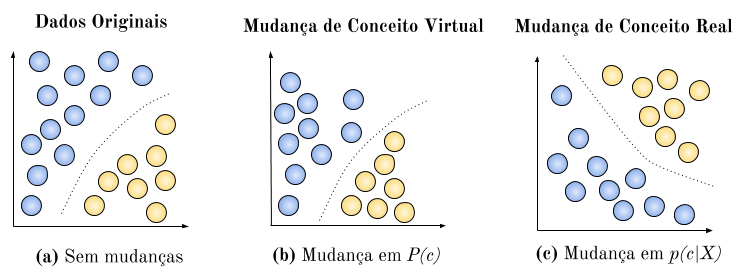
\includegraphics[scale=0.8]{imagens/concept_drift.png}
    \caption{Mudança de Conceito Virtual vs. Mudança de Conceito Real}
    \label{fig:real_and_virtual_concept_drift}
\end{center}
\end{figure}

Conforme \citeonline{Zliobaite:2010}, as mudanças de conceito podem ocorrer de forma abrupta, gradual, incremental ou recorrente.
A Figura \ref{fig:concept_drift_patterns} ilustra estes padrões,
utilizando círculos na cor azul para representar o conceito \textit{A} e círculos na cor bege para o conceito \textit{B}:

\begin{figure}[H]
\begin{center}
    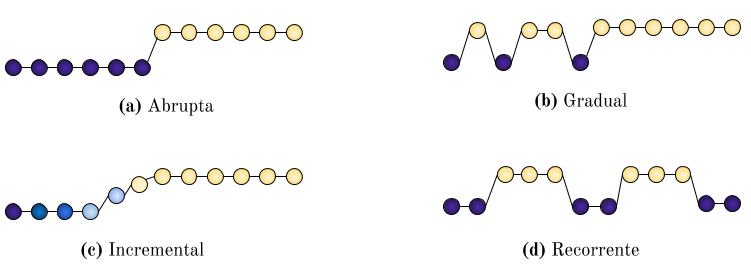
\includegraphics[scale=0.8]{imagens/concept_drift_patterns.png}
    \caption{Padrões de ocorrência de Mudanças de Conceito}
    \label{fig:concept_drift_patterns}
\end{center}
\end{figure}

Na mudança abrupta, o conceito \textit{A} é repentinamente substituído pelo conceito \textit{B} (Figura \ref{fig:concept_drift_patterns} (a)).

Na mudança gradual, ocorre uma transição mais suave entre os conceitos \textit{A} e \textit{B}.
Inicialmente, eventos pertencentes a ambos os conceitos coexistem.
Com o passar do tempo, os eventos pertencentes ao conceito \textit{A} diminuem de frequência, até pararem de ocorrer.
Por fim, os eventos pertencentes a \textit{B} se tornam predominantes (Figura \ref{fig:concept_drift_patterns} (b)).

A mudança incremental descreve a evolução de um único conceito ao longo do tempo.
Essa evolução pode ser discretizada como uma sequência de conceitos consecutivos.
Nesta sequência, cada conceito intermediário difere pouco dos seus conceitos antecessor e sucessor.
Portanto, as mudanças são notáveis apenas à longo prazo (Figura \ref{fig:concept_drift_patterns} (c)).

A mudança recorrente acontece quando um conceito anteriormente ativo reaparece após um determinado período de tempo.
Contudo, não se trata de uma sazonalidade periódica, pois não é evidente o momento no qual o conceito voltará a ser ativo (Figura \ref{fig:concept_drift_patterns} (d)).

Esta dissertação propõe um novo método baseado em Redes de Função de Base Radial e Cadeias de Markov para detecção de mudanças de conceito em fluxos contínuos de dados, independente do padrão de ocorrência.
Na próxima subseção, será apresentada a terminologia do fenômeno mudança de conceito.

\subsection{Terminologia}

O fenômeno mudança de conceito tem sido estudado em diferentes comunidades de pesquisa, incluindo Mineração de Dados,
Aprendizado de Máquina, Estatística e Recuperação de Informação \cite{Zliobaite:2010}.
Contudo, o tema apresenta diferentes nomeclaturas em cada comunidade.
Na Tabela \ref{tbl:taxonomy} são listados os termos correspondentes a mudança de conceito em cada área de pesquisa.

\begin{table*}[!ht]
    \caption{Terminologia - Mudança de Conceito \cite{Zliobaite:2010}}
    \label{tbl:taxonomy}
    \centering
    \resizebox{\textwidth}{!}{%
    \begin{tabular}[t]{ll}
    \toprule
    Área & Termos \\
    \midrule
    Mineração de Dados                  & Mudança de Conceito                        \\
    Aprendizado de Máquina              & Mudança de Conceito, Mudança de Covariável \\
    Computação Evolucionária            & Ambiente Evolutivo, Ambiente em Mudança    \\
    IA e Robótica                       & Ambiente Dinâmico                          \\
    Estatística, Séries Temporais      & Não Estacionário                           \\
    Recuperação de Informação           & Evolução Temporal                          \\
    \bottomrule
    \end{tabular}%
    }
\end{table*}

Outra fonte comum de equívocos são os termos detecção de \textit{outliers}, detecção de novidade, detecção de \textit{change points} e detecção de mudança de conceito.
Estes termos são muitas vezes utilizados de forma indistinta, mas, para o contexto deste trabalho, é importante distingui-los.

As técnicas para detecção de \textit{outliers} têm como objetivo identificar padrões de dados em desacordo com o comportamento esperado. Estes padrões são geralmente classificados como anomalias ou ruídos \cite{Chandola:2009:ADS:1541880.1541882}.

Os métodos para detecção de novidade identificam padrões ainda não observados, mas que se enquadram no comportamento esperado.
Estes métodos se diferenciam das técnicas para detecção de \textit{outliers} pois os novos padrões são incorporados ao modelo \cite{Chandola:2009:ADS:1541880.1541882}.

As estratégias para detecção de \textit{change points} identificam variações abruptas de valor, que podem representar transições entre estados, em séries temporais unidimensionais estacionárias \cite{Aminikhanghahi:2017:SMT:3086013.3086037}.

Por fim,  cabe definir o que é detecção de mudança de conceito.
Este termo abrange técnicas que monitoram a distribuição dos dados ou indicadores produzidos pelas técnicas de aprendizado aplicadas, com o objetivo de identificar variações que possam impactar a acurácia do modelo em uso \cite{Gama:2014:SCD:2597757.2523813}.

Na próxima subseção, os principais algoritmos para detecção de mudança de conceito serão discutidos.

\subsection{Algoritmos para Detecção de Mudança de Conceito}

Os algoritmos para detecção de mudança de conceito caracterizam e quantificam as mudanças de conceito através da delimitação dos instantes ou intervalos de tempo em que as mudanças ocorrem \cite{Basseville:1993:DAC:151741}.

Esses algoritmos se dividem em duas categorias, conforme a necessidade de rotulação dos dados \cite{Zliobaite:2010}:

\begin{description}
    \item[Algoritmos Explícitos/Supervisionados] Dependem da rotulação dos dados por um especialista.
    Estes rótulos são utilizados no cálculo de medidas de performance como taxa de erro e acurácia, que são monitoradas ao longo do tempo.
    Mudanças de conceito são sinalizadas quando essas medidas atingem um limite previamente definido.

    \item[Algoritmos Implícitos/Não Supervisionados] Independem da rotulação por especialistas.
    As mudanças de conceito são detectadas a partir do monitoramento de características dos próprios dados ou de indicadores produzidos pelas técnicas de aprendizado aplicadas.
    Apesar de serem mais propensos a alarmes falsos, são uma alternativa para cenários onde a obtenção de rótulos é dispendiosa, demorada ou inviável.
\end{description}

Segundo \citeonline{Gama:2014:SCD:2597757.2523813}, os algoritmos \textit{explícitos / supervisionados} podem ser segmentados em três subcategorias:

\begin{description}
    \item[Métodos Baseados em Análise Sequencial] Avaliam continuamente os indicadores de performance (por exemplo: taxa de erro) do algoritmo de aprendizado aplicado.
    A mudança de conceito é detectada quando esses indicadores atingem um limite pré-definido.
    Os algoritmos \textit{Cumulative Sum (CUSUM)}, \textit{PageHinkley (PH)} \cite{Page:CUSUM:PageHinkley:1954} e \textit{Geometric Moving Average (GMA)} \cite{Roberts:2000:CCT:338441.338464}
    são representantes desta subcategoria.

    \item[Abordagens baseadas em Estatística] Identificam mudanças de conceito através da análise de parâmetros estatísticos como média e desvio padrão associados aos resultados das predições.
    Os métodos \textit{Drift Detection Method (DDM)} \cite{GamaMCR04},
    \textit{Early Drift Detection Method (EDDM)} \cite{EDDM},
    \textit{Exponentially Weighted Moving Average (EWMA)} \cite{Ross:2012:EWM:2076039.2076307} e
    \textit{Reactive Drift Detection Method (RDDM)} \cite{Barros:RDDM:2017} são exemplos desta subcategoria.

    \item[Métodos baseados em Janelas] Utilizam uma janela de tamanho fixo para sumarizar informações passadas e uma janela deslizante para sumarizar os dados recentes.
    Uma diferença significativa entre as distribuições dessas janelas implica na ocorrência de mudança de conceito.
    Esta diferença é verificada a partir de testes estatísticos ou desigualdades matemáticas, considerando como hipótese nula a igualdade das distribuições.
    Os algoritmos
    \textit{Adaptive Windowing (ADWIN)} \cite{BifetG07},
    \textit{SeqDrift} \cite{PearsSK14:SeqDrift:2014},
    \textit{HDDMA} e \textit{HDDMW} \cite{BlancoCRBDM15:HDDMA:HDDMW:2015}
    pertencem a esta subcategoria.
\end{description}

De forma similar, os algoritmos \textit{implícitos / não supervisionados} também foram divididos em três subcategorias \cite{GONCALVES20148144}:

\begin{description}
    \item[Detecção de Novidade / Métodos de Agrupamento]
    Utilizam técnicas derivadas dos métodos de agrupamento e de detecção de \textit{outliers} para identificar padrões ainda não observados.
    A partir dessa identificação, são realizados cálculos de distância e/ou densidade para confirmar a ocorrência de mudança de conceito \cite{Ryu:Kantardzic:2012}.
    Os métodos
    \textit{OLINDDA} \cite{Spinosa:2007:OCA:1244002.1244107},
    \textit{MINAS} \cite{Faria:2013:NDA:2480362.2480515},
    \textit{Woo} \cite{Ryu:Kantardzic:2012},
    \textit{DETECTNOD} \cite{Hashemi:Hayat:DETECTNOD:2010},
    \textit{ECSMiner} \cite{Masud:2011:CNC:1978259.1978529} e
    \textit{GC3} \cite{Sethi2016b:GC3} fazem parte desta subcategoria.

    \item[Monitoramento de distribuição multivariada]
    Monitoram diretamente a distribuição dos dados para cada atributo.
    A distribuição de um conjunto de treinamento é sumarizada e utilizada como referência.
    Esta referência é, então, comparada à distribuição dos dados do conjunto atual.
    Diferenças significativas entre esses conjuntos indicam a ocorrência de mudança de conceito.
    Os algoritmos
    \textit{CoC} \cite{Lee:Magoules:CoC:2012},
    \textit{HDDDM} \cite{Ditzler:Polikar:HDDDM:2011},
    \textit{PCA-detect} \cite{Kuncheva:PCADetect:20085}
    são representantes desta subcategoria.

    \item[Monitoramento dependente de modelo]
    Requerem a aplicação de um algoritmo de classificação probabilístico,
    pois as mudanças de conceito são detectadas a partir do monitoramento da probabilidade a posteriori calculada \cite{Zliobaite:2010}.
    Esta restrição permite reduzir a ocorrência de falsos positivos e torna o processo computacionalmente eficiente, pois apenas um único fluxo univariado de valores é observado.
    Os métodos
    \textit{A-distance} \cite{Dredze:ADistance:2010585},
    \textit{CDBD} \cite{Lindstrom:CDBD:2013} e
    \textit{Margin} \cite{Dries:Margin:2009} integram esta subcategoria.
\end{description}

Por fim, a Tabela \ref{tbl:abordagens} resume as categorias, as subcategorias e as técnicas apresentadas.
O método de detecção proposto neste trabalho se enquadra na categoria de algoritmos \textit{implícitos / não supervisionados}, mais especificamente na subcategoria \textit{detecção de novidades / métodos de agrupamento}.
Na próxima seção, a ferramenta MOA, utilizada para implementar e validar o método proposto neste trabalho, é apresentada.

\begin{table}[ht]
    \caption{Resumo - Algoritmos de detecção \cite{Sethi:2017:RDC:3096751.3096864}}
    \label{tbl:abordagens}
    \centering
    \resizebox{\textwidth}{!}{%
    \begin{tabular}[t]{@{}lllll@{}}
    \toprule
    Categoria & Subcategoria & Algoritmos \\
    \midrule
    Algoritmos Explícitos/Supervisionados     & Métodos Baseados em Análise Sequencial        & \begin{tabular}[t]{@{}l@{}} Cumulative Sum (CUSUM) \\ PageHinkley (PH) \cite{Page:CUSUM:PageHinkley:1954} \\ Geometric Moving Average (GMA) \cite{Roberts:2000:CCT:338441.338464}\end{tabular}                                                                                                                        &  &  \\
    \addlinespace[2mm]
                                              & Abordagens baseadas em Estatística            & \begin{tabular}[t]{@{}l@{}} Drift Detection Method (DDM) \cite{GamaMCR04} \\  Early Drift Detection Method (EDDM) \cite{EDDM} \\  Exponentially Weighted Moving Average (EWMA) \cite{Ross:2012:EWM:2076039.2076307} \\ Reactive Drift Detection Method (RDDM) \cite{Barros:RDDM:2017} \end{tabular}                   &  &  \\
    \addlinespace[2mm]
                                              & Métodos baseados em Janelas                   & \begin{tabular}[t]{@{}l@{}} Adaptive Windowing (ADWIN) \cite{BifetG07} \\   SeqDrift \cite{PearsSK14:SeqDrift:2014} \\   HDDMA/HDDMW \cite{BlancoCRBDM15:HDDMA:HDDMW:2015} \end{tabular}                                                                                                                              &  &  \\
    \addlinespace[2mm]

    Algoritmos Implícitos/Não Supervisionados & Detecção de Novidade / Métodos de Agrupamento & \begin{tabular}[t]{@{}l@{}} OLINDDA \cite{Spinosa:2007:OCA:1244002.1244107} \\   MINAS \cite{Faria:2013:NDA:2480362.2480515} \\   Woo \cite{Ryu:Kantardzic:2012} \\   DETECTNOD \cite{Hashemi:Hayat:DETECTNOD:2010} \\   ECSMiner \cite{Masud:2011:CNC:1978259.1978529} \\   GC3 \cite{Sethi2016b:GC3} \end{tabular}  &  &  \\
    \addlinespace[2mm]
                                              & Monitoramento de distribuição multivariada    & \begin{tabular}[t]{@{}l@{}} CoC \cite{Lee:Magoules:CoC:2012} \\ HDDDM \cite{Ditzler:Polikar:HDDDM:2011} \\ PCA-detect \cite{Kuncheva:PCADetect:20085} \end{tabular}                                                                                                                                                   &  &  \\
    \addlinespace[2mm]
                                              & Monitoramento dependente de modelo            & \begin{tabular}[t]{@{}l@{}} A-distance \cite{Dredze:ADistance:2010585} \\ CDBD \cite{Lindstrom:CDBD:2013} \\ Margin \cite{Dries:Margin:2009} \end{tabular}                                                                                                                                                            &  &  \\
    \bottomrule
    \end{tabular}%
    }
\end{table}

\subsection{Ferramenta - MOA}

Atualmente, o \textit{MOA – Massive Online Analysis}\footnote{https://moa.cms.waikato.ac.nz/} é o principal framework para mineração de dados em fluxos contínuos \cite{Bifet:2010:MMO:1756006.1859903}.
O framework é de código-aberto\footnote{https://github.com/Waikato/moa} e apresenta uma comunidade bastante ativa e crescente.
A aplicação é composta por uma ampla coleção de algoritmos da área de Aprendizado de Máquina, contemplando técnicas de classificação, regressão, agrupamento, busca por padrões, detecção de \textit{outliers}, detecção de mudanças de conceito e sistemas de recomendação.
Além das implementações, também estão disponíveis rotinas para avaliação dessas técnicas.
A aplicação é desenvolvida em Java, o que permite a sua execução nos principais sistemas operacionais e a integração com o projeto WEKA \cite{Hall:2009:WDM:1656274.1656278}.

O MOA divide as suas funcionalidades em tarefas (\textit{tasks}).
Estas tarefas podem ser executadas a partir da interface gráfica (GUI) ou por linha de comando.
A interface gráfica permite executar múltiplas tarefas de forma concorrente,
controlar suas execuções e visualizar os resultados parciais.
A tela principal da aplicação é demonstrada na Figura \ref{fig:moa}.

\begin{figure}[H]
\begin{center}
    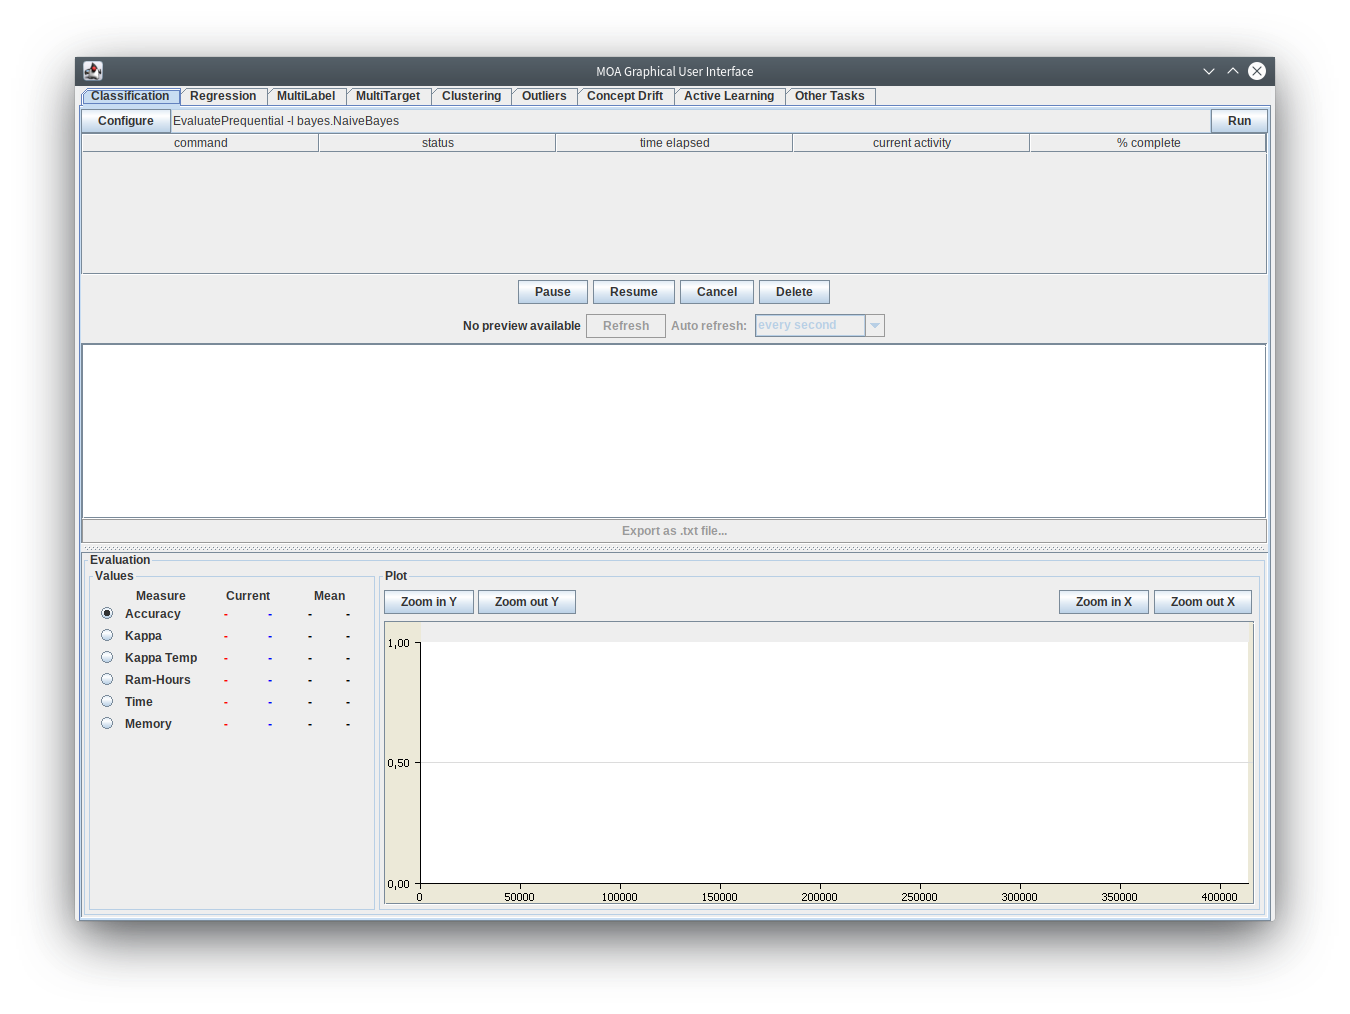
\includegraphics[scale=0.4]{imagens/moa.png}
    \caption{MOA - Tela Inicial}
    \label{fig:moa}
\end{center}
\end{figure}

A aplicação é capaz de ler arquivos em formato ARFF\footnote{\textit{Attribute-Relation File Format}}, além de permitir a produção de fluxos de dados dinamicamente, através de geradores.
Alguns dos geradores de fluxo disponíveis no MOA são:
\textit{Random Trees} \cite{Domingos:2000:MHD:347090.347107}
\textit{SEA} \cite{Street:2001:SEA:502512.502568},
\textit{STAGGER} \cite{Schlimmer1986},
\textit{Rotating Hyperplane} \cite{Wang:2003:MCD:956750.956778},
\textit{Random RBF},
\textit{LED} \cite{Gama:2003:ADT:956750.956813},
\textit{Waveform} \cite{Gama:2003:ADT:956750.956813},
 e \textit{Function} \cite{Jin:2003:EDT:956750.956821}.

Outra funcionalidade importante do framework é a possibilidade de adicionar mudanças de conceito a fluxos estacionários existentes.
Esse processo é realizado através de uma função sigmóide, que modela o evento de mudança de conceito como uma combinação balanceada de duas distribuições homogêneas,
que caracterizam os conceitos-alvo antes e depois da mudança.
Além destes conceitos, o usuário também pode definir o momento da mudança e a sua duração \cite{Bifet:2010:MMO:1756006.1859903}.

A arquitetura do framework é modular, o que permite a implementação de novos algoritmos de forma trivial.
Para tanto, basta estender a classe abstrata \textit{AbstractChangeDetector} e implementar o algoritmo desejado.
A janela de configuração deste detector, similar a Figura \ref{fig:moa_detector}, será criada dinamicamente, a partir dos atributos definidos na classe.

\begin{figure}[H]
\begin{center}
    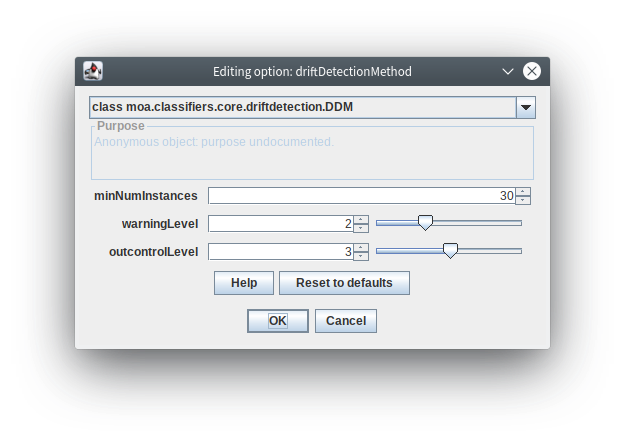
\includegraphics[scale=1]{imagens/detector.png}
    \caption{MOA - Configuração detector}
    \label{fig:moa_detector}
\end{center}
\end{figure}

O MOA possui implementações dos principais algoritmos para detecção de mudanças de conceito presentes na literatura.
Além das implementações, a ferramenta também disponibiliza rotinas de avaliação, que analisam a acurácia e o desempenho desses métodos.

Nesta pesquisa, o MOA foi utilizado para realização do experimento com dados sintéticos.
Os conjuntos de dados usados foram gerados a partir da ferramenta.
A técnica proposta foi implementada e comparada aos principais algoritmos disponíveis.
Por fim, os testes realizados foram avaliados atráves da classe \textit{BasicConceptDriftPerformanceEvaluator}.

\section{Redes de Função de Base Radial}

Uma Rede de Função de Base Radial (redes RBF, em português,  ou \textit{radial basis function network, RBF network}, em inglês) pode ser definida como um modelo de múltiplas camadas alimentadas adiante (\textit{feedforward}),
capaz de analisar padrões complexos e resolver problemas não-linearmente separáveis, utilizando uma abordagem de aproximação de funções.
Estas redes têm como principal diferencial a sua forma de ativação, realizada através do cálculo da distância entre o dado e um centro definido \cite{Braga:RedesNeuraisTeoriaAplicacoes}.

A arquitetura de uma rede de função de base radial, em sua forma mais básica, envolve três camadas.
A camada de entrada representa os atributos do problema. As unidades dessa camada não realizam processamento e simplesmente distribuem as entradas para os neurônios na camada intermediária.
A camada intermediária, única camada oculta da rede, é constituída por funções de ativação de base radial, que atuam como os neurônios da rede.
Por fim, a camada de saída pondera, através de pesos, os resultados da camada intermediária, agregando-os linearmente para compor a resposta final da rede \cite{Rojas:1996:NNS:235222}.
A Figura \ref{fig:rbg_arq} demonstra essa arquitetura.

Na literatura, as funções Gaussianas (Função \ref{eq:gaussiana}) são as funções de ativação mais usuais em redes RBF, sendo definidas por seus centros e larguras:

\begin{equation}
    \label{eq:gaussiana}
    \varphi (v_{i})=e^{-(\sigma r)^{2}}
\end{equation}

onde, $r$ é a distância euclidiana ($\|\mathbf {v_{i}} - \mathbf {c_{i}}\|$), $v$ é o valor de entrada, $c_i$ representa o centro e $\sigma$ é o parâmetro limitador do raio.

\begin{figure}[H]
\begin{center}
    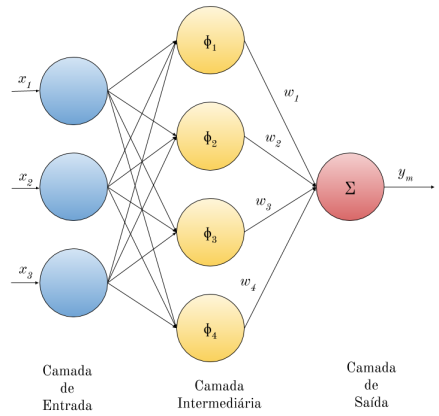
\includegraphics[scale=1]{imagens/rbf_arq.png}
    \caption{Arquitetura RBF}
    \label{fig:rbg_arq}
\end{center}
\end{figure}

A modelagem das redes RBF define a entrada como um vetor de números reais ${x} \in {R} ^{n}$ e o resultado da rede como uma função escalar desse vetor $\varphi : {R} ^{n} \to {R}$.
Esta função é obtida a partir da combinação linear dos resultados das funções de ativação (Equação \ref{eq:rbf1}).

\begin{equation} \label{eq:rbf1}
    \varphi ({x})=\sum _{{i=1}}^{N}a_{i}\rho (||{x}-{c}_{i}||)
\end{equation}

onde $N$ é o número de neurônios na camada intermediária, ${c}_{i}$ é o centro do neurônio $i$, $||\ldots||$ é a norma euclidiana e $a_{i}$ é o peso (bias) atribuído ao neurônio para realização da combinação linear.

A técnica proposta nesta dissertação utiliza uma rede RBF adaptada.
No método proposto, apenas as camadas inicial e intermediária são aplicadas.
Esta adaptação é possível, pois a camada intermediária cria, implicitamente, durante o processo de ativação, grupos com os dados recebidos ao longo do tempo.
Dessa forma, quando o centro ativo do agrupamento formado é alterado, uma possível mudança de conceito é sinalizada.

Além da rede RBF adaptada, o método proposto também utiliza uma Cadeia de Markov para modelar as transições entre centros e obter tolerância a ruídos.
As Cadeias de Markov serão apresentadas na próxima seção.

\section{Cadeias de Markov}

\ldots

\section{Monitoramento Ocular - Classificação de Fixações e Sacadas}

\ldots

\section{Considerações Finais}

Neste capítulo foram apresentados os principais conceitos utilizados na pesquisa.
Foram discutidos conceitos de Fluxos Contínuos de Dados,
técnicas de Aprendizado de Máquina,
Mudança de Conceito,
Técnicas de Detecção e Redes de Função de Base Radial.
Por fim, foram apresentados os trabalhos relacionados encontrados na literatura.
No próximo capítulo, o plano de pesquisa será detalhado.

\xchapter{Trabalhos Relacionados}{} \label{trabalhos_relacionados}

\section{Considerações Iniciais}

\ldots

Além das referências básicas apresentadas neste capítulo, foi realizada uma pesquisa na literatura em busca de trabalhos que propõem métodos para identificação de mudanças de conceito, de forma online e independente de rótulos, em fluxos contínuos de dados. Também foram estudadas técnicas que pudessem subsidiar o desenvolvimento de novos algoritmos que atendam a esses requisitos.

Inicialmente, foram analisados os algoritmos \textit{Implícitos / Não Supervisionados} pertencentes a subcategoria \textit{Detecção de Novidade / Métodos de Agrupamento}. Estes algoritmos são descritos a seguir.

% Métodos de Detecção de Novidade utilizam cálculos de distância e/ou densidade da informação para detectar padrões de dados ainda não observados. Estes métodos são capazes de identificar exemplos que podem provocar incerteza, demandando uma avaliação mais apurada. Os algoritmos atribuem a estes exemplos um rótulo \textbf{Desconhecido} para indicar que estas amostras não se enquadram na visão corrente dos dados \cite{Spinosa:2007:OCA:1244002.1244107}.
% Técnicas de Agrupamento e Detecção de Outliers são estratégias populares para implementar tais métodos, pois resumem os dados correntes e aplicam métricas de dissimilaridade para identificar novos padrões \cite{Ryu:Kantardzic:2012}.

O algoritmo \textit{OnLIne Novelty and Drift Detection Algorithm} (OLINDDA) utiliza a técnica de agrupamento \textit{K-means} para monitorar e se adaptar ao surgimento de novos padrões \cite{Spinosa:2007:OCA:1244002.1244107}.
Os exemplos recepcionados são incluídos em uma fila e são periodicamente agrupados. Os grupos resultantes desse processamento definem se os exemplos devem ser incorporados a um grupo existente ou formar um novo grupo.

O algoritmo MINAS, proposto por \citeonline{Faria:2013:NDA:2480362.2480515}, atua de forma similar ao algoritmo OLLINDA, contudo utiliza \textit{micro clusters} obtidos a partir da aplicação de uma técnica de agrupamento específica para fluxos contínuos de dados (CluStream) e estende a abordagem para permitir a aplicação em problemas multiclasse.

O algoritmo DETECTNOD \cite{Hashemi:Hayat:DETECTNOD:2010} utiliza um modelo de clusterização para delimitar os exemplos observados.
Uma representação compacta desses grupos é produzida através da Transformada Discreta de Cosseno. Esta representação é utilizada, em conjunto com o algoritmo de vizinho mais próximo, para aproximar novos exemplos.
Estes exemplos são categorizados como desvios ou novidades, conforme o grau de similaridade calculado.

Os algoritmos Woo \cite{Lee:Wang:Ryu:2007} e ECSMiner \cite{Masud:2011:CNC:1978259.1978529} também se baseiam no conceito de \textit{micro clusters}. A técnica Woo atribui um classificador para cada cluster formado. Estes classificadores são utilizados para verificar a similaridade de novos exemplos em relação ao cluster. Exemplos que não se enquadram em nenhum grupo são marcados como suspeitos e passam a ter sua densidade monitorada. Um número crescente de vizinhos no raio dos exemplos monitorados indica o surgimento de um novo conceito, induzindo o retreino do modelo e ajuste do centróide do agrupamento.
O ECSMiner \cite{Masud:2011:CNC:1978259.1978529} utiliza o conceito de Outliers Filtrados, que se refere a amostras que estão fora do limite de todos os clusters existentes, em uma abordagem similiar ao algoritmo Woo.

O algoritmo GC3 \cite{Sethi2016b:GC3} estende a ideia de \textit{micro clusters} ao aplicar um algoritmo de agrupamento baseado em grade e densidade. Dessa forma, novos padrões são identificados a partir do surgimento de novas áreas de alta densidade.

Os algoritmos baseados em técnicas de detecção de novidade utilizam métodos de agrupamento para identificar padrões emergentes. Portanto, também apresentam dificuldade para lidar com alta dimensionalidade e/ou dados binários, por dependerem do cálculo de distância, e são computacionalmente custosos.

A segunda etapa da pesquisa analisou técnicas para detecção de mudanças de conceito em séries temporais que atuam de forma online. Estas técnicas também são comumente denominadas como técnicas para detecção de \textit{change points}. A maioria dos trabalhos identificados se baseia no monitoramento dos valores residuais da aplicação de um modelo. Nesta abordagem, um modelo estatístico ou de Aprendizado de Máquina é aplicado a um conjunto de observações extraídas da série temporal, representando um conceito.
Assume-se que se não houver mudança de conceito, os valores residuais dessa aplicação devem ser estacionários. Os trabalhos identificados são apresentados a seguir.

\citeonline{Yamanishi:2002:UFD:775047.775148} propõem um método de detecção online capaz de identificar outliers e mudanças de conceito em séries temporais.
A abordagem aplica um modelo autoregressivo aos dados e atualiza os parâmetros de forma incremental, para que o peso de exemplos passados diminua ao longo do tempo. Atribui-se uma pontuação para cada observação, calculada com base na função de perda. Esta pontuação indica o grau de desvio do dado em relação ao modelo aplicado. Pontuações elevadas indicam alta possibilidade de que o dado seja um outlier. A detecção de mudança de conceito é feita através do monitoramento da média das funções de perda ao longo da série temporal. Todavia, esta abordagem só é aplicável a séries temporais com comportamento autoregressivo, o que limita o seu escopo de uso.

\citeonline{GOMBAY2009715} propõem um método diferente, também online, para detecção de mudanças em séries temporais autoregressivas, baseado no monitoramento dos parâmetros do modelo. Um adaptação do método CUSUM \cite{Page:CUSUM:PageHinkley:1954} é aplicada para identificar alterações nos parâmetros. A hipótese nula do algoritmo assume que estes parâmetros devem permanecer estacionários ao longo do tempo. Esta hipótese é testada para cada nova observação recepcionada e a mudança de conceito é sinalizada quando a diferença ultrapassa um limiar estabelecido. Esta abordagem também apresenta limitação de escopo, pois é aplicável apenas a séries temporais autoregressivas.

A utilização de valores residuais para detecção de mudanças de conceito  apresenta desvantagens. Por serem baseados na acurácia do modelo aplicado, estes métodos sofrem influência de problemas ocorridos durante a parametrização ou fase de treinamento. Em teoria, o monitoramento direto de características dos dados pode permitir uma identificação de mudanças de conceito mais robusta.

Poucos estudos utilizam as características das séries temporais para identificar mudanças de conceito. Neste contexto, o trabalho proposto por  \citeonline{Boracchi2014ExploitingSF} se destaca por apresentar um método de detecção de mudanças de conceito em séries temporais que atua de forma online, baseando-se no monitoramento da característica de auto-similaridade da série.
Entretanto, o método proposto tem como principal limitação o fato de ser especializado para séries que apresentam auto-similaridade e periodicidade. Além disso, a abordagem utiliza uma considerável quantidade de memória, pois armazena uma sequência de dados que representa o comportamento estável ou regular da série temporal.

Para cenários nos quais os fluxos de dados não apresentam as propriedades esperadas pelas técnicas discutidas anteriormente, \citeonline{StableApproachToDetectConceptDrift:Mello} propõem um novo método para detecção de mudanças de conceito que atua de forma online.
Este trabalho se diferencia por utilizar um algoritmo de agrupamento hierárquico estável, conforme a propriedade proposta por \citeonline{Carlsson:2010:CSC:1756006.1859898}.
A abordagem cria janelas consecutivas de dados. A técnica de agrupamento é aplicada em cada janela e os dendogramas resultantes comparados, a fim de identificar mudanças de conceito na distribuição dos dados.

As técnicas para detecção de mudanças de conceito são, geralmente, aplicadas para minimizar o intervalo entre a ocorrência da mudança e a atualização do modelo aplicado. Diante disso, um método de detecção ideal deve:

\begin{itemize}
    \item ser transparente para o usuário, detectando e informando explicitamente sobre a ocorrência de mudanças;
    \item ser computacionalmente eficiente;
    \item atuar de forma online, buscando minimizar o atraso de atualização do modelo; e
    \item basear-se em características dos dados que reflitam os conceitos presentes.
\end{itemize}

Por fim, a pesquisa realizada evidenciou a inexistência de técnicas que atendam a esses requisitos e que sejam computacionalmente eficientes, independentes de rótulos e aplicáveis a fluxos de dados de qualquer natureza. Este projeto de trabalho de mestrado tem como objetivo tentar preencher esta lacuna na literatura, através da proposição de um novo método, baseado em Redes de Função de Base Radial,  para identificação de mudanças de conceito em fluxos contínuos de dados.

\section{Considerações Finais}

\ldots

\xchapter{RBFC\element{hain}}{} \label{rbfchain}

\section{Considerações Iniciais}

Este capítulo descreve como este projeto de mestrado será desenvolvido.
A abordagem proposta utiliza Redes de Função de Base Radial para detectar mudanças de conceito em fluxos contínuos de dados.
Espera-se que a utilização de redes RBF permita detectar mudanças em tempo de execução, de forma computacionalmente eficiente e independente de rótulos.
A seguir, são apresentados detalhes sobre cada etapa do desenvolvimento do projeto.

\section{RBFChain}

Nos últimos anos, a quantidade de dados produzidos por sistemas computacionais tem crescido de forma exponencial \cite{idc_report}.
Parte significativa dessas informações é produzida na forma de fluxos contínuos de dados, que são sequências potencialmente infinitas e de alta frequência \cite{Aggarwal:2006:DSM:1196418}.

Devido a esse crescimento, pesquisadores passaram a utilizar técnicas de Aprendizado de Máquina para extrair informações úteis de grandes volumes de dados.
Essas técnicas precisaram ser adaptadas para contextos com fluxos contínuos, pois estes cenários apresentam severas restrições de tempo de execução e de uso dos recursos computacionais.

Contudo, as adaptações propostas não tratam alterações na distribuição dos dados ou no contexto do processo gerador do fluxo.
Estas alterações são denominadas mudanças de conceito e podem afetar negativamente a acurácia do algoritmo \cite{Gama:2014:SCD:2597757.2523813}.

Para mitigar este problema, métodos de detecção de mudanças de conceito foram desenvolvidos.
Estes métodos identificam o momento da mudança com maior precisão, permitindo que o modelo de decisão seja atualizado de forma eficiente.

Entretanto, as técnicas de detecção encontradas na literatura apresentam limitações ao serem aplicadas em cenários com fluxos contínuos de dados.
Os métodos de detecção supervisionados/explícitos necessitam que o rótulo correto de cada exemplo processado seja informado, o que pode torná-los inviáveis, por causa do custo e/ou do tempo para rotulação.
Enquanto que as técnicas não supervisionadas/implícitas têm dificuldade para atender às restrições de tempo de execução e de uso dos recursos computacionais desses cenários.
Diante disso, este trabalho propõe uma nova abordagem para detecção de mudanças de conceito baseada em Redes de Função de Base Radial.

As redes RBF podem ser definidas como redes neurais multicamadas, alimentadas adiante, capazes de analisar padrões complexos e resolver problemas que não são linearmente separáveis \cite{Braga:RedesNeuraisTeoriaAplicacoes}.
A arquitetura básica dessas redes é composta por três camadas.
A camada de entrada recepciona os dados e repassa para a camada seguinte.
A camada intermediária realiza a ativação dos neurônios através de funções de base radial.
E, por fim, a camada de saída produz o resultado final da rede através de uma combinação linear dos resultados da camada intermediária \cite{Rojas:1996:NNS:235222}.

Este trabalho de mestrado utiliza apenas as camadas inicial e intermediária dessa arquitetura.
Isto ocorre, pois a camada intermediária forma, implicitamente, grupos (\textit{clusters}) durante o processo de ativação.
Este agrupamento possui um centro ativo que muda conforme o valor processado.
O algoritmo desenvolvido nesta pesquisa monitora o agrupamento formado para identificar quando esse centro é alterado.
Estas alterações são utilizadas como indícios de possíveis mudanças de conceito.

O método proposto, denominado \textit{RBFChain}, utiliza a função Gaussiana para ativação dos neurônios e requer a definição de dois parâmetros:
\textit{$\sigma$}, responsável por limitar o raio da radial, e \textit{$\lambda$}, que define um limiar para ativação de um centro.
A técnica é descrita na forma de pseudocódigo em Algoritmo \ref{alg:algoritmo},
tendo sido também implementada na linguagem Java\footnote{\url{https://git.io/fjGuv}}, para realização dos experimentos na plataforma MOA.

\vspace{7pt}
\begin{algorithm}[H]
    \SetAlgoLined
    \Entrada{$valor, \sigma, \lambda$}
    \Saida{booleano indicando a ocorrência ou não de mudança de conceito}
    \Inicio{
     $centros \longleftarrow ()$; $centroAtual \longleftarrow null$; $centroAtivo \longleftarrow null$\\
     $mudanca \longleftarrow falso$

     \ParaTodo{centro}{
         $ativacao \longleftarrow gaussiana(valor, centro, \sigma)$\\
         \Se{$ativacao >= \lambda$}{
            $centroAtivo \longleftarrow centro$ \\
            $\lambda \longleftarrow ativacao$ \\
         }
    }
    \Se{$centroAtivo == null$}{
        $centros \longleftarrow valor$ \\
        $centroAtivo \longleftarrow valor$ \\
    }
    \Se{$centroAtual \neq centroAtivo$}{
        $centroAtual \longleftarrow centroAtivo$ \\
        $mudanca \longleftarrow verdadeiro$ \\
    }
    \Retorna{mudanca}\\
    \BlankLine
    \BlankLine
    }

    \caption{\textsc{RBFChain}}
    \label{alg:algoritmo}
\end{algorithm}
\vspace{7pt}

Para exemplificar a execução do algoritmo proposto neste projeto, considere o conjunto $S = \{0.11, 0.12, 0.13, 0.34, 0.45, 0.47, 0.33, 0.25, 0.14, 0.10\}$ como fonte de dados.
Para este exemplo, os parâmetros foram definidos de forma empírica. O parâmetro \textit{$\sigma$} foi definido com o valor $0.2$ e o parâmetro \textit{$\lambda$} foi fixado em $0.6$.
A seguir, será descrito o comportamento do algoritmo para cada dado recebido a partir de $S$.

No instante $T1$, o valor $0.11$ é recepcionado. Como não existem centros estabelecidos, o valor é definido como centro e ativado.
Em $T2$ e $T3$ são recebidos, respectivamente, os valores $0.12$ e $0.13$ que são imediatamente vinculados ao centro atualmente ativo ($0.11$), pois seus valores de ativação foram maiores que $0.6$ ($\lambda$).

No instante $T4$, o valor $0.34$ não atinge o valor mínimo de ativação (\textit{$\lambda$}) para ser vinculado ao centro ativo ($0.11$).
Dessa forma, o valor é definido como um novo centro e ativado.
Devido a alteração do centro ativo, o algoritmo sinaliza a ocorrência de mudança de conceito.

Os valores dos instantes $T5$, $T6$, $T7$ e $T8$ são vinculados ao último centro ativo ($0.34$).
Contudo, em $T9$, o valor $0.14$ é recebido e apresenta maior valor de ativação para o centro $0.11$, que é reativado.
Assim, uma nova mudança de conceito é sinalizada.
Finalmente, o valor do instante $T10$, $0.10$, é vinculado ao centro ativo ($0.11$).

A Figura \ref{fig:funcionamento_algoritmo} apresenta esse comportamento graficamente.
Os círculos na cor amarela representam valores vinculados ao primeiro centro estabelecido ($0.11$ no momento $T1$),
enquanto os de cor lilás foram ativados pelo segundo centro definido ($0.34$ em $T4$).
As linhas verticais tracejadas, de cor vermelha, indicam a ocorrência de mudança de conceito.

\begin{figure}[H]
\begin{center}
    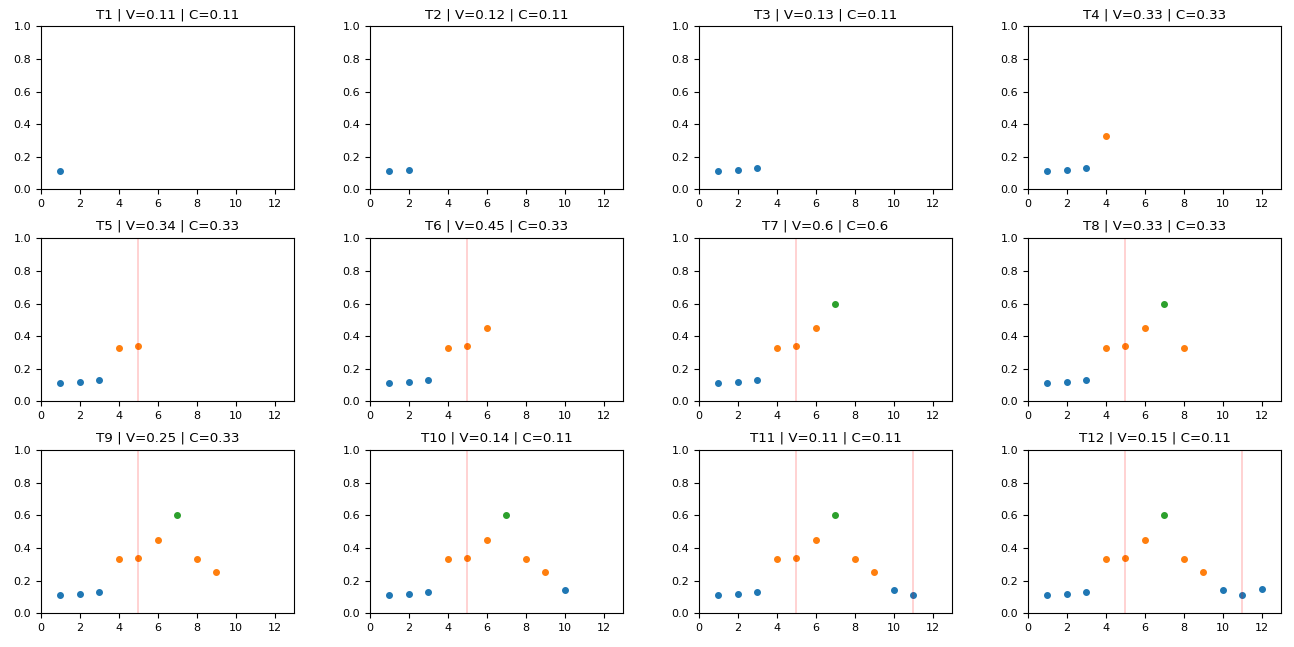
\includegraphics[width=\textwidth]{imagens/funcionamento_algoritmo.png}
    \caption{Exemplo de funcionamento do algoritmo}
    \label{fig:funcionamento_algoritmo}
\end{center}
\end{figure}

% \section{Atividades de Pesquisa}

% A Tabela \ref{cronograma} apresenta o cronograma das atividades planejadas para a realização da pesquisa. Atividades concluídas são representadas pelo símbolo $X$ e as futuras por $\bullet$.

% \begin{table}[htbp]
% \begin{center}
% \caption{Cronograma de atividades}     % mude aqui para seu título da tabela
% \label{cronograma} % para referencia no texto.
% \resizebox{\textwidth}{!}{ % abre resizebox, setar tabela da largura da página.
% \begin{tabular}{|c|l|l|l|l|l|l|l|l|l|l|l|l|l|l|l|l|l|l|l|l|l|l|l|l|}
% \hline
% \multicolumn{1}{|c|}{\multirow{2}{*}{Atividades}} & \multicolumn{24}{c|}{Meses} \\ \cline{2-25}
% \multicolumn{1}{|c|}{} & 01 & 02 & 03 & 04 & 05 & 06 & 07 & 08 & 09 & 10 & 11 & 12 & 13 & 14 & 15 & 16 & 17 & 18 & 19 & 20 & 21 & 22 & 23 & 24 \\ \hline
% %\rowcolor[HTML]{EFEFEF}

% 1-Disciplinas & X & X & X & X & X & X & X & X & X & X & ~ & ~ & ~ & ~ & ~ & ~ & ~ & ~ & ~ & ~ & ~ & ~ & ~ & ~ \\ \hline
% 2-Revisão da Literatura & ~ & ~ & ~ & ~ & ~ & ~ & X & X & X & X & X & X & ~ & ~ & ~ & ~ &  ~ & ~ & ~ & ~ & ~ & ~ & ~ & ~ \\ \hline
% 3-Experimentos  & ~ & ~ & ~ & ~ & ~ & ~ & ~ & ~ & X & X & X  & X & $\bullet$ & $\bullet$ & $\bullet$ & $\bullet$ & ~ & ~ & ~ & ~ & ~ & ~ & ~ & ~ \\ \hline
% 4-Análise dos Resultados & ~ & ~ & ~ & ~ & ~ & ~ & ~ & ~ & ~ & ~ & X & X & ~  & ~  & ~ & $\bullet$ & $\bullet$ & $\bullet$ & ~ & ~ & ~ & ~ & ~ & ~ \\ \hline
% 5-Escrita da qualificação & ~ & ~ & ~ & ~ & ~ & ~ & ~ & ~ & ~ & X & X & X & ~ & ~ & ~ & ~ & ~ & ~ & ~ & ~ & ~ & ~ & ~ & ~ \\ \hline
% 6-Estágio docente & ~ & ~ & ~ & ~ & ~ & ~ & ~ & ~ & ~ & ~ & ~ & ~ & ~ & ~ & ~ & $\bullet$ & $\bullet$ & $\bullet$ & $\bullet$ & $\bullet$ & $\bullet$ & ~ & ~ & ~ \\ \hline
% 7-Pesquisa Orientada & ~ & ~ & ~ & ~ & ~ & ~ & X & X & X & X & X & X & $\bullet$ & $\bullet$ & $\bullet$ & $\bullet$ & $\bullet$ & $\bullet$ & $\bullet$ & $\bullet$ & $\bullet$ & $\bullet$ & $\bullet$ & $\bullet$ \\ \hline
% 8-Apresentação da qualificação & ~ & ~ & ~ & ~ & ~ & ~ & ~ & ~ & ~ & ~ & ~ & ~ & $\bullet$ & ~ & ~ & ~ & ~ & ~ & ~ & ~ & ~ & ~ & ~ & ~ \\ \hline
% 9-Escrita de artigos& ~ & ~ & ~ & ~ & ~ & ~ & ~ & ~ & ~ & ~ & ~ & ~ & ~  & ~ & ~ & ~ & ~ & $\bullet$ & $\bullet$ & ~ & ~ & ~ & ~ & ~ \\ \hline
% 10-Escrita da dissertação& ~ & ~ & ~ & ~ & ~ & ~ & ~ & ~ & ~ & X & X & X & ~ & ~ & ~ & ~ & $\bullet$ & $\bullet$ & $\bullet$ & $\bullet$ & $\bullet$ & $\bullet$ & $\bullet$ & $\bullet$ \\ \hline
% 11- Defesa da dissertação& ~ & ~ & ~ & ~ & ~ & ~ & ~ & ~ & ~ & ~ & ~ & ~ & ~ & ~ & ~ & ~ & ~ & ~ & ~ & ~ & ~ & ~ & ~ & $\bullet$ \\ \hline

% \hline
% \end{tabular}
% } % fecha resizebox
% \end{center}
% \end{table}

% Para a conclusão da atividade 1,
% o Programa de Pós-Graduação em Ciência da Computação (PGCOMP) da Universidade Federal da Bahia (UFBA) exige que um mestrando obtenha um total de 18 créditos em disciplinas.
% Nos semestres 2018.1 e 2018.2, foram obtidos os créditos exigidos ao cursar as disciplinas:
% MATD74 -- Algoritmos e Grafos, MATE32 -- Tópicos em Inteligência Computacional II, MATE64 -- Seminários Científicos, MATE65 -- Fundamentos de Pesquisa em Ciência da Computação I,
% MATE10 -- Tópicos em Inteligência Computacional I e MATE84 -- Tópicos em Fundamentos da Computação IV.

% A segunda atividade planejada neste cronograma foi realizada a partir da disciplina MATE65 -- Fundamentos de Pesquisa em Ciência da Computação I
% e nos meses subsequentes. Além disso, durante a execução desta tarefa foi realizada a prova de proficiência em inglês.

% As atividades 3 e 4 do cronograma consistem na realização dos experimentos e análise dos resultados.
% Essas atividades foram divididas em duas partes.
% A primeira contém apenas experimentos preliminares que foram realizados para validar esta proposta de trabalho.
% Nesta parte, conjuntos de dados sintéticos foram analisados conforme apresentado no Capítulo \ref{experimentos_iniciais}.
% A segunda parte dos experimentos e suas análises serão realizadas após a qualificação.

% As atividades 5 e 8 estão relacionadas com o componente curricular MATD75 -- Exame de qualificação. A atividade 5 refere-se à escrita deste texto e as atividades 6 e 7 representam os componentes curriculares MATA32 -- Estágio Docente e MATA31 -- Pesquisa Orientada, respectivamente. A atividade 8 está relacionada à apresentação desta qualificação de mestrado.

% A escrita de artigos, listada no item 9 do cronograma, será realizada com base nos resultados gerados com os experimentos (Atividades $3$ e $4$) e nas contribuições obtidas com a apresentação da qualificação. Por fim, como requisito para a defesa de dissertação, fica pendente a atividade MATE93 - Defesa de Proposta de Mestrado, a qual se refere aos itens 10 e 11 da Tabela \ref{cronograma}.

\section{Considerações Finais}

Neste capítulo, apresentou-se de maneira detalhada o projeto de pesquisa, o plano de atividades e o cronograma planejado para a conclusão do mestrado.
No próximo capítulo, serão discutidos os experimentos iniciais, realizados com o objetivo de analisar a viabilidade da proposta de mestrado.

\xchapter{Experimentos e Resultados}{} \label{experimentos_iniciais}
\section{Considerações Iniciais}

Este capítulo apresenta um conjunto de experimentos preliminares realizados com dados sintéticos, cujo objetivo foi demonstrar a viabilidade da proposta de mestrado.
%
Os resultados obtidos se mostraram promissores, indicando que o tema de pesquisa deve continuar a ser investigado.
%
A próxima seção apresenta como os dados sintéticos foram produzidos para condução dos experimentos.

\section{Configuração dos Experimentos}
\label{sec:configuracao_experimentos}

Os fluxos de dados sintéticos foram produzidos através de classes geradoras do framework MOA e salvos em arquivos no formato ARFF. %, permitindo para que pudessem ser reutilizados entre os experimentos.
Cada fluxo produzido representa até dois conceitos e é composto por 2.500 observações, com valores entre 0 e 1.
O restante desta seção apresenta as classes geradoras utilizadas, as modificações realizadas e os parâmetros aplicados.

A classe geradora \textit{AbruptChangeGenerator} produz fluxos de dados sintéticos com mudanças de conceito abruptas.
Os fluxos gerados simulam as mudanças através da intercalação de sequências com o valor $0.2$ e sequências com o valor $0.8$, conforme o tamanho definido para os conceitos.
Com o objetivo de tornar os dados produzidos mais próximos da realidade, essa classe foi alterada\footnote{\url{https://git.io/fjGEj}} para permitir a adição de um ruído randômico, com amplitude configurável, para cada exemplo produzido.
A versão com suporte a ruído foi utilizada nos experimentos para produção do fluxo com mudanças abruptas.
O gerador foi parametrizado para produzir exemplos não binários, com conceitos formados com 400 instâncias e ruído limitado ao intervalo $[-0.1, 0.2]$ seguindo uma distribuição uniforme.

% Esta configuração é apresentada na Figura \ref{fig:abrupt_change_generator}.

% \begin{figure}[H]
%     \begin{center}
%         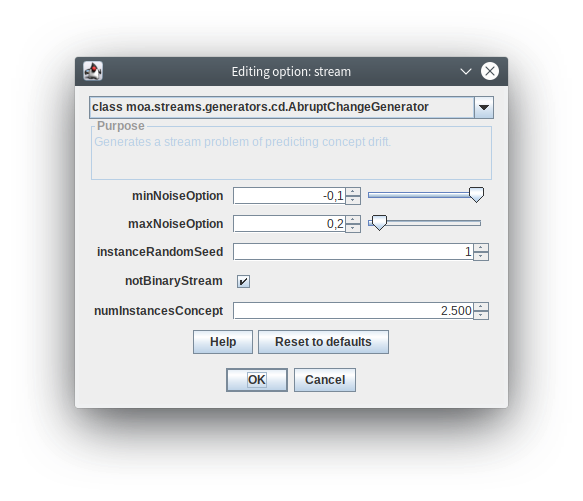
\includegraphics[width=\textwidth]{imagens/abrupt_change_generator.png}
%         \caption{Parametrização da classe \textit{AbruptChangeGenerator}}
%         \label{fig:abrupt_change_generator}
%     \end{center}
% \end{figure}

A classe \textit{GradualChangeGenerator} produz fluxos sintéticos com mudanças de conceito graduais.
Durante sua configuração, percebeu-se uma limitação, pois a classe só gera uma mudança gradual, independente do tamanho dos conceitos.
Para superar esta limitação, a classe foi modificada\footnote{\url{https://git.io/fjGue}} para gerar uma quantidade de mudanças coerente com o tamanho definido.
A classe modificada foi utilizada para gerar o fluxo sintético com mudanças graduais utilizado nos experimentos,
sendo parametrizada para produzir exemplos não binários e conceitos compostos por 400 instâncias.

% A Figura \ref{fig:gradual_change_generator} apresenta a tela de configuração da aplicação.

% \begin{figure}[H]
%     \begin{center}
%         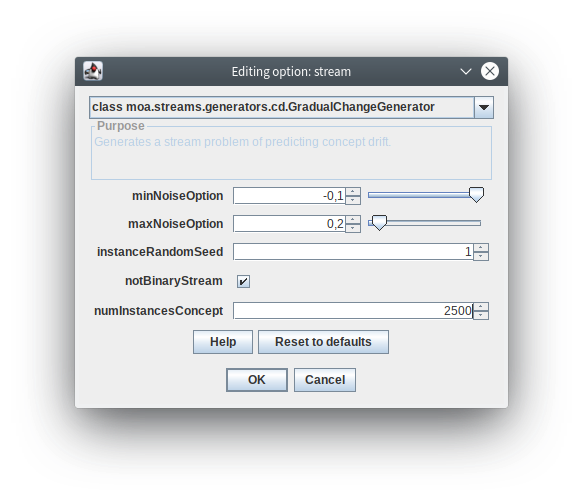
\includegraphics[width=\textwidth]{imagens/gradual_change_generator.png}
%         \caption{Parametrização da classe \textit{GradualChangeGenerator}}
%         \label{fig:gradual_change_generator}
%     \end{center}
% \end{figure}

Por fim, a classe \textit{NoChangeGenerator}, que produz fluxos sem ocorrência de mudanças de conceito, também foi modificada\footnote{\url{https://git.io/fjGu3}} para permitir a incidência de ruído nos resultados gerados.
Esta versão foi utilizada para produzir um fluxo sintético sem mudanças, com ruído entre $[-0.1, 0.1]$.

\section{Critérios de avaliação}

A classe de avaliação \textit{BasicConceptDriftPerformanceEvaluator}, pertencente ao framework MOA, foi utilizada para avaliar o método proposto neste trabalho.
Esta classe permite mensurar a acurácia e o desempenho de algoritmos para detecção de mudanças de conceito.
Para utilizá-la, é necessário construir uma tarefa do tipo \textit{EvaluateConceptDrift} através da aba \textit{Concept Drift}, presente na tela inicial da aplicação.
Para condução dos experimentos deste trabalho, a tarefa \textit{EvaluateConceptDrift} foi configurada conforme descrito na Tabela \ref{tbl:configuracao_tarefa}.

\begin{center}
    \begin{table}[h]
    \caption{Configuração da classe \textit{BasicConceptDriftPerformanceEvaluator}}
    \label{tbl:configuracao_tarefa}
    \resizebox{\textwidth}{!} {%
    \begin{tabular}{llm{7.5cm}}
    \toprule
    Parâmetro & Valor & Observação \\
    \midrule
    learner          & ChangeDetectorLearner  &  O algoritmo de detecção de mudanças de conceito a ser testado é definido no atributo \textit{driftDetectionMethod} da classe \textit{ChangeDetectorLearner}.                   \\
    stream           & ARFFFileStream         &  Caminho para um dos arquivos \textit{ARFF} descrito na seção anterior. O atributo \textit{classIndex} deve ser definido como $0$, pois não existem rótulos nestes conjuntos de dados.  \\
    instanceLimit    & $-1$                            &  Desabilita o limite de instâncias a serem processadas.  \\
    timeLimit        & $-1$                            &  Desabilita o limite de tempo de execução.  \\
    sampleFrequency  & \hspace{3mm}$1$                 &  Uma linha de resultado do avaliador deve ser gerada para cada instância processada.  \\
    \bottomrule
    \end{tabular}
    }
    \end{table}
\end{center}

A classe de avaliação utilizada produz diversos indicadores referentes a acurácia e performance do algoritmo executado.
A Tabela \ref{tbl:indicadores_analisado} apresenta os indicadores analisados neste trabalho.

\begin{center}
    \begin{table}[h]
    \caption{Indicadores analisados}
    \label{tbl:indicadores_analisado}
    \resizebox{\textwidth}{!} {%
    \begin{tabular}{lm{10cm}}
    \toprule
    Indicador & Observação \\
    \midrule
    Tempo de Processamento    &  Tempo médio (seg.) de processamento por instância. \\
    Mudanças Existentes       &  Quantidade de mudanças existentes. \\
    Mudanças Detectadas       &  Quantidade de mudanças detectadas corretamente. \\
    Falso-positivos           &  Quantidade de mudanças detecatadas erroneamente. \\
    Atraso de Detecção        &  Quantidade média de instâncias até a detecção. \\
    \bottomrule
    \end{tabular}
    }
    \end{table}
\end{center}

\section{P\element{ettitt}}

Durante a revisão da literatura, investigou-se a aplicabilidade das técnicas para detecção de \textit{changing points} em problemas de detecção de mudança de conceito.
Para tanto, foi realizada a implementação, no framework MOA\footnote{\url{https://git.io/fj8xu}}, de um novo algoritmo baseado no método estatístico proposto por \citeonline{Pettitt}.

O método de Pettitt é um teste não paramétrico, no qual se verifica se duas amostras $Y_1,...,Y_t$ e $Y_{t+1},...,Y_T$ são da mesma população. A estatística $U_{t,T}$ faz uma contagem do número de vezes que um membro da primeira amostra é maior que um membro da segunda.
A estatística $U_{t,T}$ é obtida através da Equação \ref{eq:pettitt}:

\begin{equation}
    \label{eq:pettitt}
    U_{t,T} = U_{t-1,T} + \sum_{j=1}^{T}sgn(Y_t-Y_j)
\end{equation}

Onde $t = 2,....,T$; $sgn(x) = 1$ para $x>0$; $sgn(x)= 0$ para $x=0$ e $sgn(x)=-1$ para $x<0$.
A estatística $U_{t,T}$ é então calculada para os
valores de $1 \leq t \leq T$ e a estatística $k(t)$ do teste de
Pettitt é o máximo valor absoluto de $U_{t,T}$.

Os testes foram executados com os conjuntos de dados sintéticos produzidos na Seção \ref{sec:configuracao_experimentos}. Os resultados obtidos são apresentados a seguir, na Tabela \ref{tbl:pettitt}.

\begin{center}
    \begin{table}[H]
    \caption{Resultados - Método de Pettitt}
    \label{tbl:pettitt}
    \resizebox{\textwidth}{!} {%
    \begin{tabular}{llllll}
    \toprule
    Conjunto de Dados & Tempo de processamento & Mudanças Existentes & Mudanças Detectadas & Falso-positivos & Atraso de Detecção \\
    \midrule
    Sem mudanças           &  $3.19$ & $0$ & $0$ & $4$ & $-$ \\
    Mudanças Abruptas      &  $2.09$ & $6$ & $3$ & $2$ & $132$ \\
    Mudanças Incrementais  &  $1.48$ & $6$ & $4$ & $2$ & $133$ \\
    \bottomrule
    \end{tabular}
    }
    \end{table}
\end{center}

A análise dos resultados demonstra que o algoritmo se mostrou propenso à produção de falsos-positivo e, em comparação aos outros algoritmos abordados neste trabalho, computacionalmente ineficiente.

Por não apresentar resultados competitivos em relação ao estado da arte, esta linha de pesquisa foi suspensa, permitindo que os esforços se voltassem para a análise da aplicação de Redes de Função de Base Radial para detecção de mudanças de conceito.

\section{RBFC\element{hain}}

Esta seção apresenta um conjunto de experimentos realizados com o objetivo de validar o algoritmo desenvolvido nesta pesquisa, denominado RBFChain.
Embora os experimentos ainda não sejam suficientes para comprovar a hipótese proposta,
a análise empírica aqui apresentada evidencia a importância de analisar a aplicação de Redes de Função de Base Radial para detecção de mudanças de conceito em fluxos contínuos de dados.

Para execução dos experimentos, foram utilizados três conjuntos de dados sintéticos, conforme descrito na seção \ref{sec:configuracao_experimentos}.
Além disso, os seguintes algoritmos foram utilizados para comparação: CUSUM, PageHinkley e ADWIN.
A Tabela \ref{tbl:parametros_algoritmos} lista os parâmetros utilizados para cada algoritmo.

\begin{center}
    \begin{table}[H]
    \caption{Parâmetros utilizados para cada algoritmo}
    \label{tbl:parametros_algoritmos}
    \resizebox{\textwidth}{!} {%
    \begin{tabular}{lm{10cm}}
    \toprule
    Algoritmo & Parâmetros \\
    \midrule
    RBFChain                  &  $\sigma = 2$; $\lambda = 0.5$ \\
    CUSUM                     &  $MinNumInstances = 30; \delta = 0.005; \lambda = 50$ \\
    PageHinkley               &  $MinNumInstances = 30; \delta = 0.005; \lambda = 50; \alpha = 1$ \\
    ADWIN                     &  $\delta = 0.002$ \\
    \bottomrule
    \end{tabular}
    }
    \end{table}
\end{center}

O primeiro experimento utilizou o fluxo de dados sintético sem mudanças de conceito, a fim de avaliar a tendência de produção de falsos-positivo.
O resultado desta análise pode ser visto na Tabela \ref{tbl:exp1}.

\begin{center}
    \begin{table}[H]
    \caption{Experimento 1 - Fluxo sem mudanças de conceito}
    \label{tbl:exp1}
    \resizebox{\textwidth}{!} {%
    \begin{tabular}{llllll}
    \toprule
    Algoritmo & Tempo de processamento & Mudanças Existentes & Mudanças Detectadas & Falso-positivos & Atraso de Detecção \\
    \midrule
    RBFChain          &  $0.22$ & $0$ & $0$ & $0$ & $-$ \\
    CUSUM                     &  $0.31$ & $0$ & $0$ & $0$ & $-$ \\
    PageHinkley               &  $0.24$ & $0$ & $0$ & $0$ & $-$ \\
    ADWIN                     &  $0.21$ & $0$ & $0$ & $0$ & $-$ \\
    \bottomrule
    \end{tabular}
    }
    \end{table}
\end{center}

Como pode ser observado, todos algoritmos testados demonstraram tolerância a ruídos e não indicaram nenhum falso positivo.
Quanto a performance, o algoritmo proposto obteve a segunda melhor média em tempo de processamento. Superado pelo algoritmo ADWIN, por uma pequena margem.
O comportamento dos algoritmos e do conjunto de dados utilizado é apresentado graficamente na Figura \ref{fig:exp_sem_mudancas}.

\begin{figure}[ht]
\begin{center}
    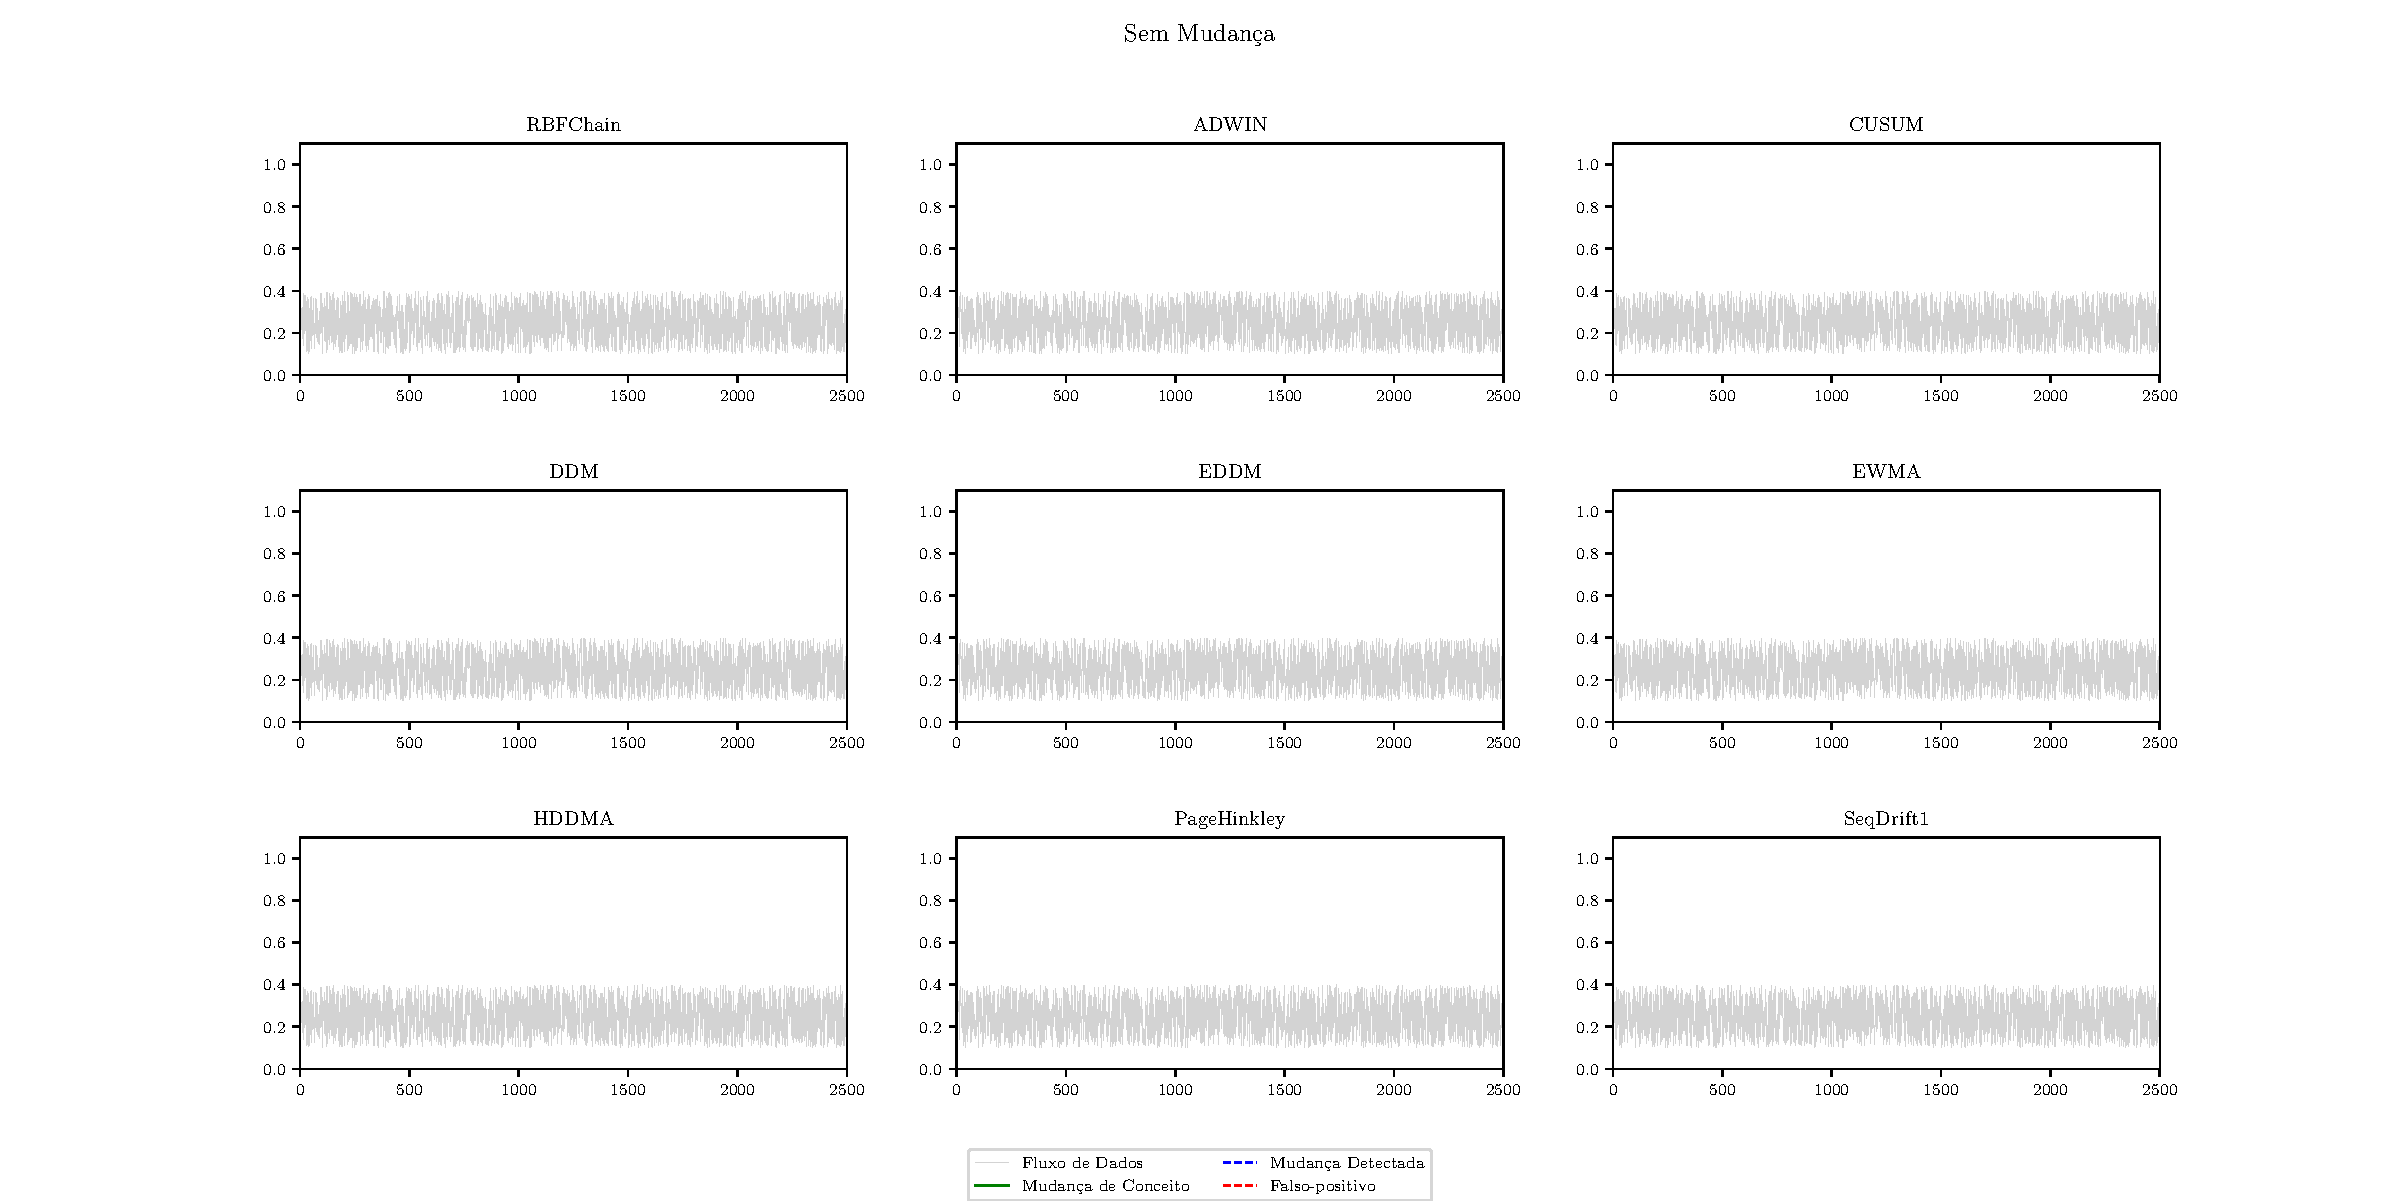
\includegraphics[width=\textwidth]{imagens/nochange.pdf}
    \caption{Representação Gráfica - Sem mudanças de conceito}
    \label{fig:exp_sem_mudancas}
\end{center}
\end{figure}

Em seguida, utilizou-se a base de dados com mudanças abruptas como base de testes.
Os resultados obtidos são apresentados na Tabela \ref{tbl:exp2}.

\begin{center}
    \begin{table}[H]
    \caption{Experimento 2 - Fluxo com mudanças de conceito abruptas}
    \label{tbl:exp2}
    \resizebox{\textwidth}{!} {%
    \begin{tabular}{llllll}
    \toprule
    Algoritmo & Tempo de processamento & Mudanças Existentes & Mudanças Detectadas & Falso-positivos & Atraso de Detecção \\
    \midrule
    RBFChain          &  $0.23$ & $6$ & $6$    & $0$    & $1$ \\
    CUSUM                     &  $0.29$ & $6$ & $3$    & $0$    & $68$ \\
    PageHinkley               &  $0.22$ & $6$ & $1$    & $0$    & $17$ \\
    ADWIN                     &  $0.21$ & $6$ & $2052$ & $2046$ & $9$ \\
    \bottomrule
    \end{tabular}
    }
    \end{table}
\end{center}

Ao analisar este resultado, verifica-se que o algoritmo proposto neste trabalho identificou todas as mudanças de conceito existentes no fluxo sem indicar nenhum falso-positivo, sendo também o algoritmo com menor atraso de detecção.
No quesito performance, a técnica desenvolvida obteve o terceiro melhor resultado.
Paralelamente, os outros algoritmos analisados apresentaram baixa acurácia.
O algoritmo CUSUM detectou apenas metade das mudanças e apresentou a maior taxa de atraso.
Enquanto o método PageHinkley detectou apenas uma mudança.
Por fim, o algoritmo ADWIN apresentou maior eficiência computacional e apesar de detectar as 6 mudanças existentes,
mostrou-se hipersensível, pois foram detectados 2046 falsos-positivo.

Os resultados do segundo experimento são demonstrados graficamente na Figura \ref{fig:exp_abrupta}. Nesta imagem, as linhas sólidas na cor verde representam as mudanças de conceito existentes no conjunto de dados analisado. As linhas tracejadas azuis representam mudanças de conceito identificadas corretamente, enquanto que as linhas tracejadas de cor vermelha representam falsos-positivo.

\begin{figure}[H]
\begin{center}
    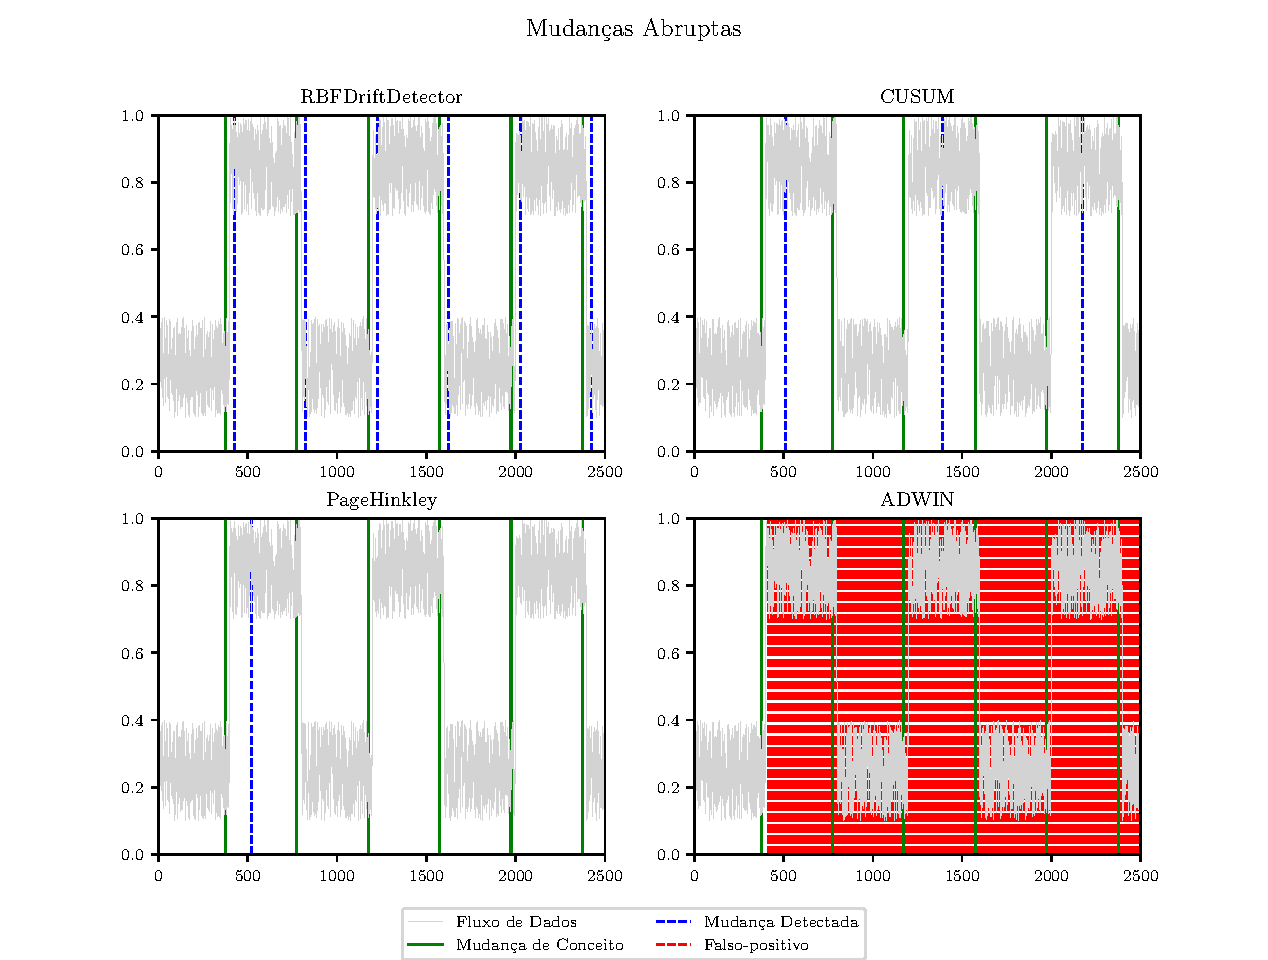
\includegraphics[width=\textwidth]{imagens/abrupt.pdf}
    \caption{Representação Gráfica - Mudanças Abruptas}
    \label{fig:exp_abrupta}
\end{center}
\end{figure}

O último experimento realizado utilizou o fluxo sintético com mudanças de conceito graduais.
Seu resultado é demonstrado na Tabela \ref{tbl:exp3}.

\begin{center}
    \begin{table}[ht]
    \caption{Experimento 3 - Fluxo com mudanças de conceito graduais}
    \label{tbl:exp3}
    \resizebox{\textwidth}{!} {%
    \begin{tabular}{llllll}
    \toprule
    Algoritmo & Tempo de processamento & Mudanças Existentes & Mudanças Detectadas & Falso-positivos & Atraso de Detecção \\
    \midrule
    RBFChain          &  $0.24$ & $6$ & $5$    & $1$    & $171$ \\
    CUSUM                     &  $0.65$ & $6$ & $3$    & $0$    & $32$ \\
    PageHinkley               &  $0.26$ & $6$ & $1$    & $0$    & $4$ \\
    ADWIN                     &  $0.27$ & $6$ & $2244$ & $2238$ & $1$ \\
    \bottomrule
    \end{tabular}
    }
    \end{table}
\end{center}

Neste experimento, o algoritmo RBFChain identificou 5 das 6 mudanças existentes e sinalizou um falso-positivo.
Ainda assim, obteve a melhor acurácia, apesar de apresentar a maior taxa de atraso.
Os outros algoritmos analisados apresentaram comportamentos similares aos do experimento anterior.
O algoritmo CUSUM identificou metade das mudanças.
O método PageHinkley identificou apenas uma alteração de conceito.
E, finalmente, o algoritmo ADWIN voltou a se mostrar muito sensível, ao identificar $2238$ falsos-positivo.

Por fim, o comportamento do conjunto de dados e dos algoritmos neste último experimento é apresentado na Figura \ref{fig:exp_gradual}.
Na imagem, as linhas sólidas na cor verde representam as mudanças de conceito existentes no conjunto de dados analisado. As linhas tracejadas azuis representam mudanças de conceito identificadas corretamente, enquanto que as linhas tracejadas de cor vermelha representam falsos-positivo.

\begin{figure}[ht]
\begin{center}
    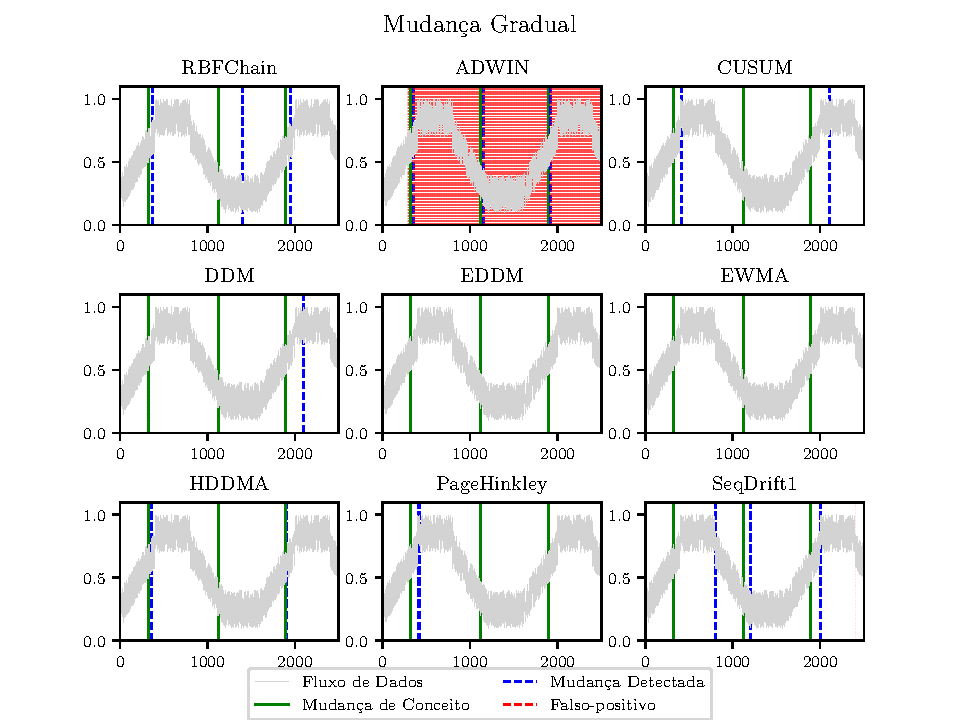
\includegraphics[width=\textwidth]{imagens/gradual.pdf}
    \caption{Representação Gráfica - Mudanças Graduais}
    \label{fig:exp_gradual}
\end{center}
\end{figure}

\section{Considerações Finais}

\ldots

\xchapter{Conclusões e Trabalhos Futuros}{} \label{conclusoes_e_trabalhos_futuros}

\section{Discussões}

\ldots

Nesta seção foram apresentados os resultados dos experimentos iniciais deste trabalho de pesquisa,
os quais visavam confirmar a aplicabilidade das Redes de Função de Base Radial na detecção de mudanças de conceito em fluxos contínuos de dados.

As seguintes etapas estão previstas para serem executadas:
i) realizar experimentos com fluxos recorrentes e incrementais;
ii) integrar uma cadeia de Markov ao método proposto, permitindo a análise do comportamento das mudanças e o aprimoramento da acurácia das detecções;
iii) implementar os algoritmos OLINDDA, MINAS e DETECNOD para serem comparados;
iv) implementar e validar o algoritmo no framework Tornado; e
v) alterar o algoritmo para permitir que o centro se desloque dentro do grupo formado.
Espera-se ainda realizar uma aplicação prática da abordagem proposta, utilizando-a em um conjunto de dados oriundo de um sistema do mundo real.

\section{Trabalhos Futuros}

\ldots

%% Parte pos-textual
\backmatter

% Bibliografia
% É aconselhável utilizar o BibTeX a partir de um arquivo, digamos "biblio.bib".
% Para ajuda na criação do arquivo .bib e utilização do BibTeX, recorra ao
% BibTeXpress em www.cin.ufpe.br/~paguso/bibtexpress
\bibliographystyle{abntex2-alf}
\bibliography{biblio}

% Apendices
% Comente se naoo houver apendices
% \appendix

%\xchapter{Exemplo de Ap\^endice}{} %sem preambulo
%\lipsum
% Eh aconselhavel criar cada apendice em um arquivo separado, digamos
% "apendice1.tex", "apendice.tex", ... "apendiceM.tex" e depois
% inclui--los com:
%\xchapter{Decomposição das séries temporais}{} %sem preambulo
\label{apendice1}
\section{Considerações Iniciais}
Neste apêndice consta as 40 séries temporais utilizadas nos experimentos mostrados no Capitulo \ref{experimentos}. As séries foram divididas em 4 tipos conforme a Tabela \ref{series}, onde o tipo representa um conjunto de 10 séries senoide ou cossenoide, sendo acrescida de ruído ou acrescida de ruído e tendência.
Nas imagens são representadas, a séries original,   seu componente determinístico e seu componente estocástico, os quais foram extraídos após a decomposição.
\section{Séries TIPO 1}
10 séries cossenoide com ruído ao longo da série.
\graphicspath{{imagens/}}
\begin{figure}[H]
\begin{center}
  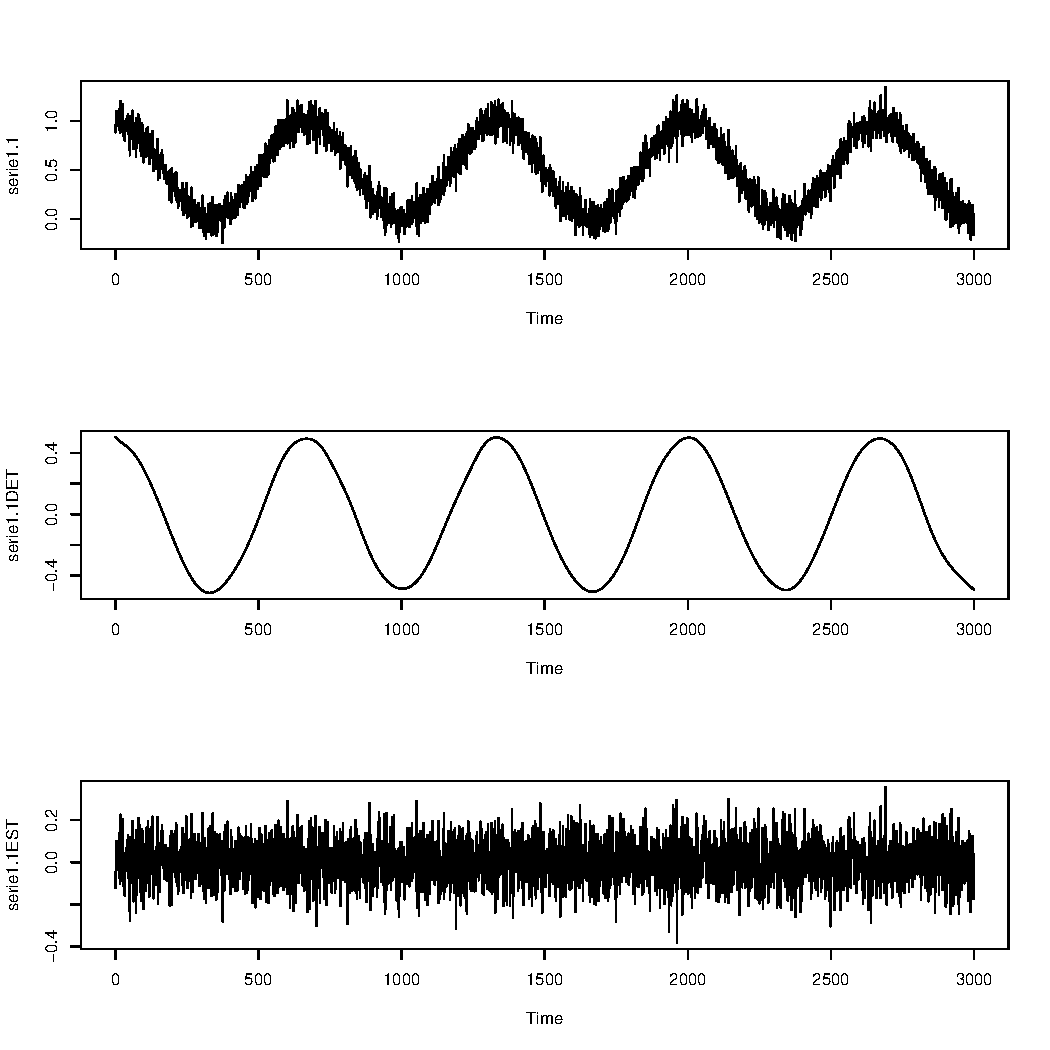
\includegraphics[scale=0.43]{serie1_1.pdf} \quad
  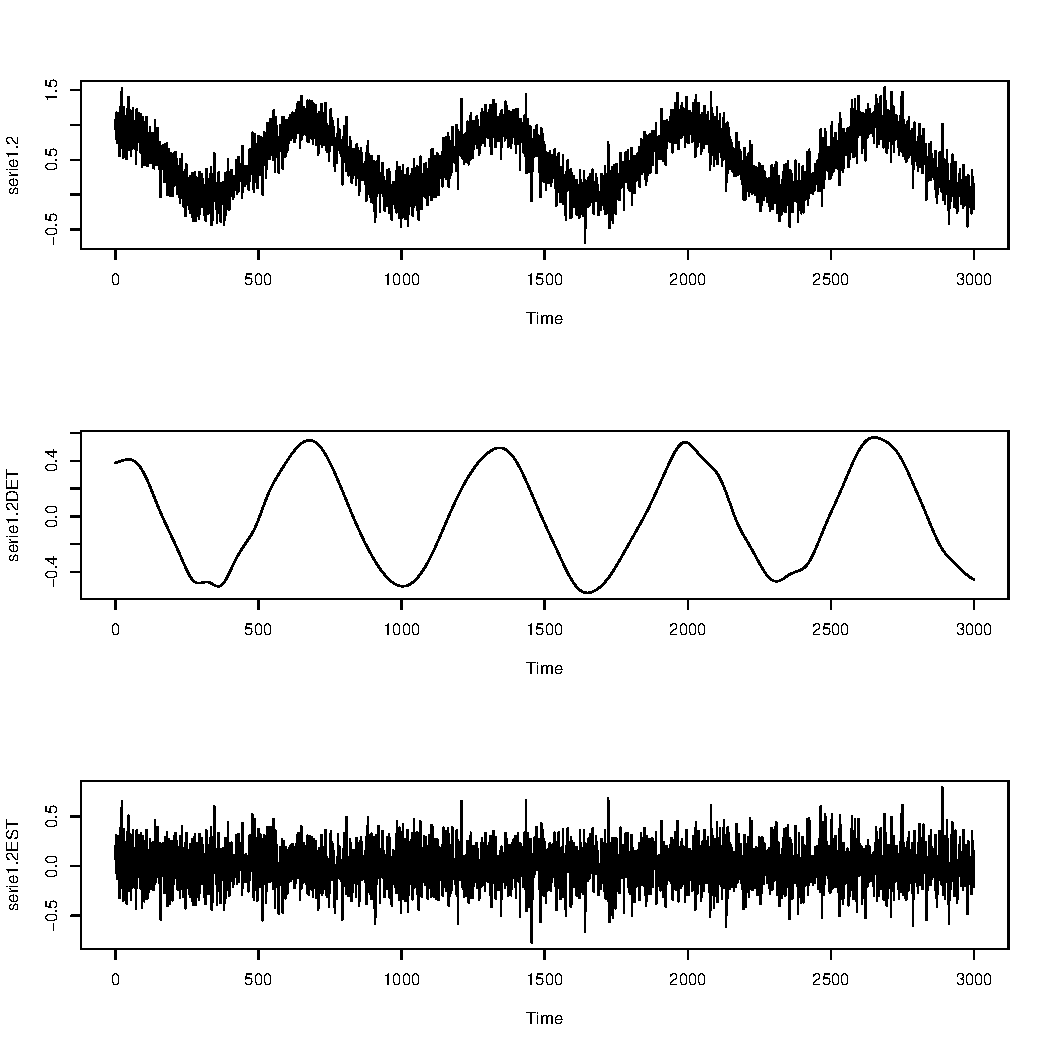
\includegraphics[scale=0.43]{serie1_2.pdf}
  \caption{Série 1.1 e Série 1.2}

\end{center}
\end{figure}

\graphicspath{{imagens/}}
\begin{figure}[H]
\begin{center}
  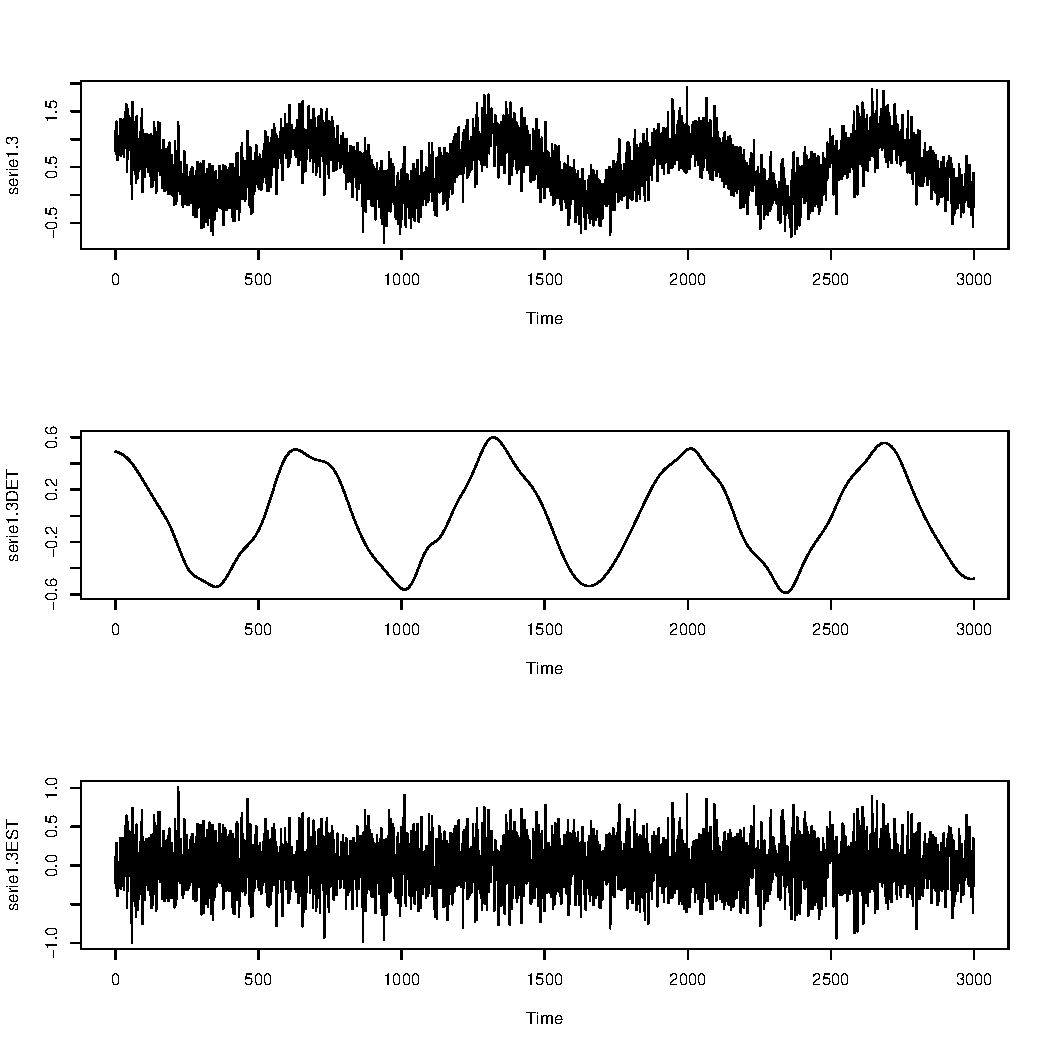
\includegraphics[scale=0.43]{serie1_3.pdf} \quad
  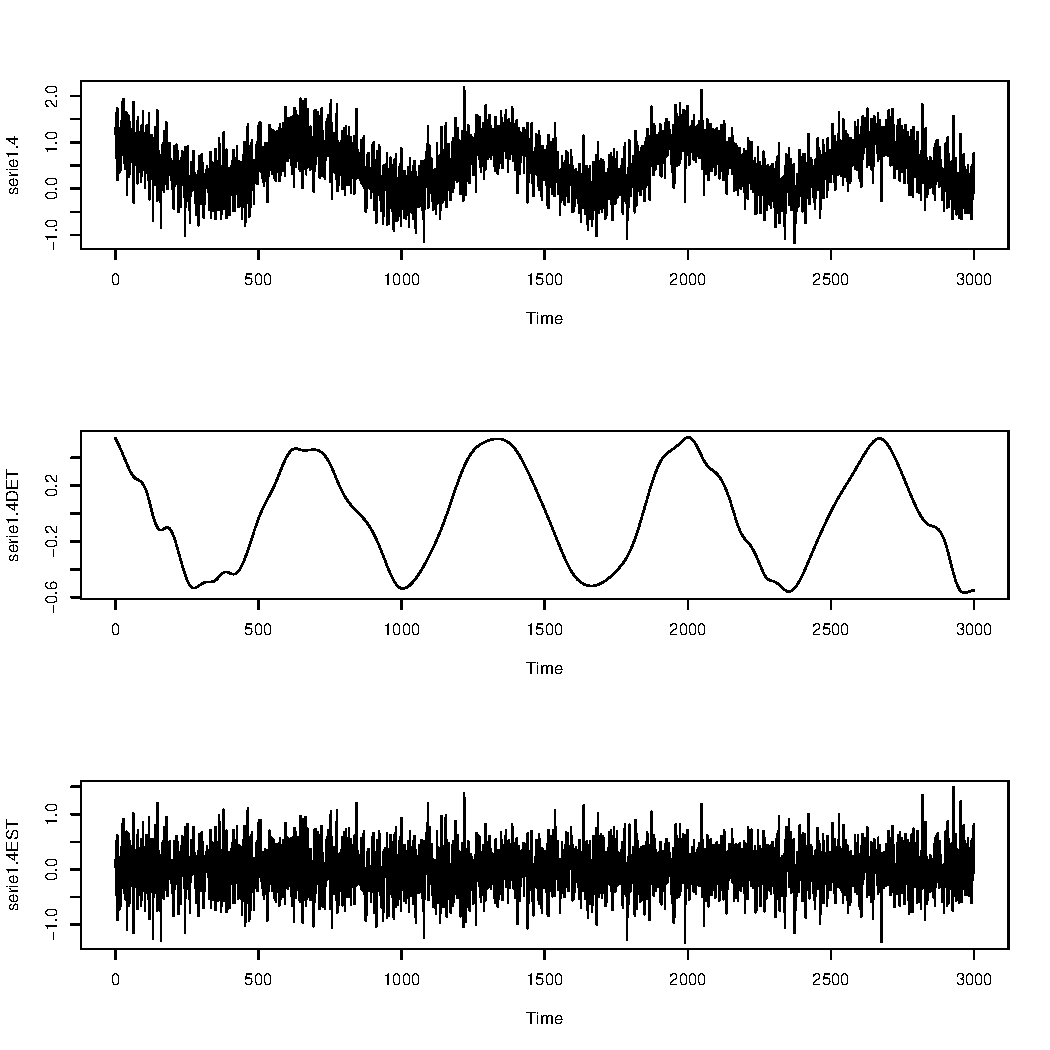
\includegraphics[scale=0.43]{serie1_4.pdf}
  \caption{Série 1.3 e Série 1.4}

\end{center}
\end{figure}

\graphicspath{{imagens/}}
\begin{figure}[H]
\begin{center}
  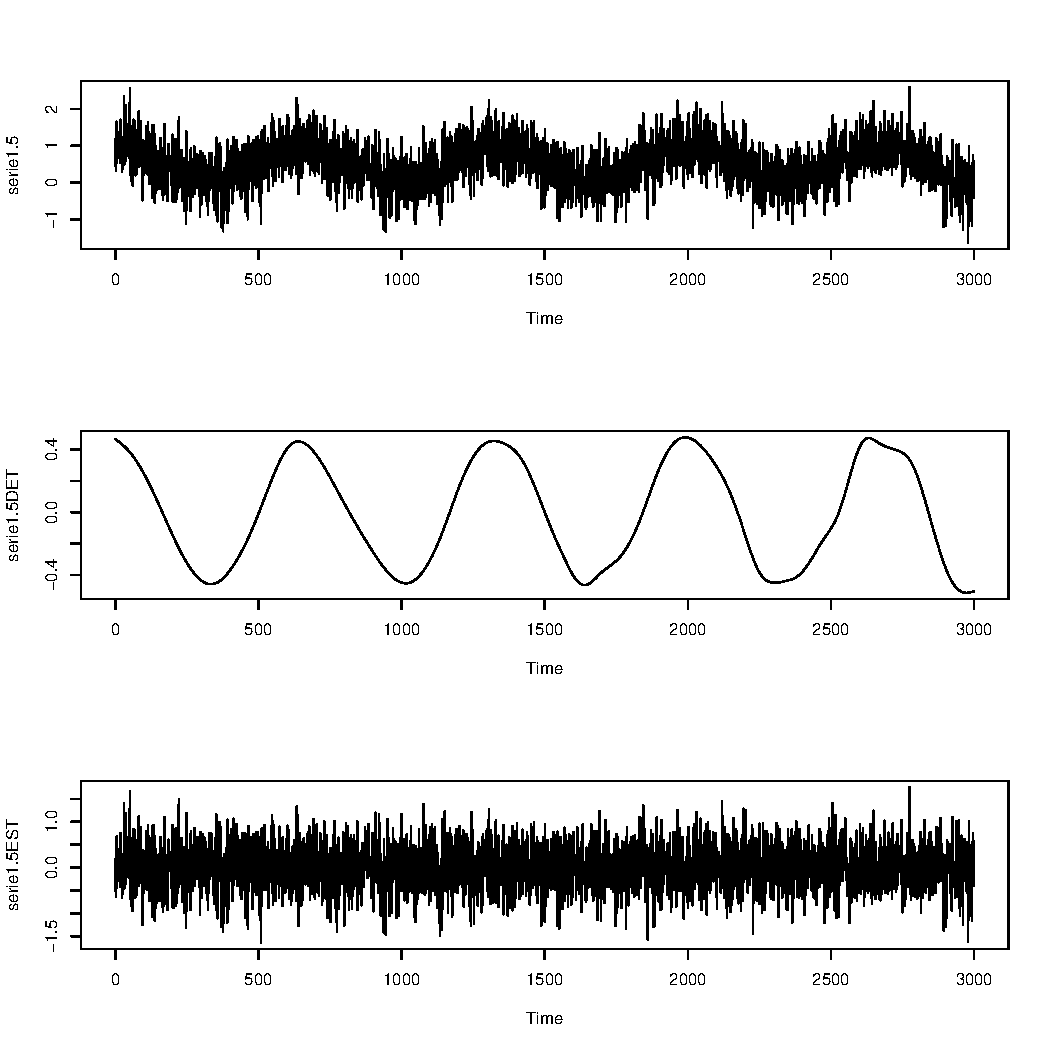
\includegraphics[scale=0.43]{serie1_5.pdf} \quad
  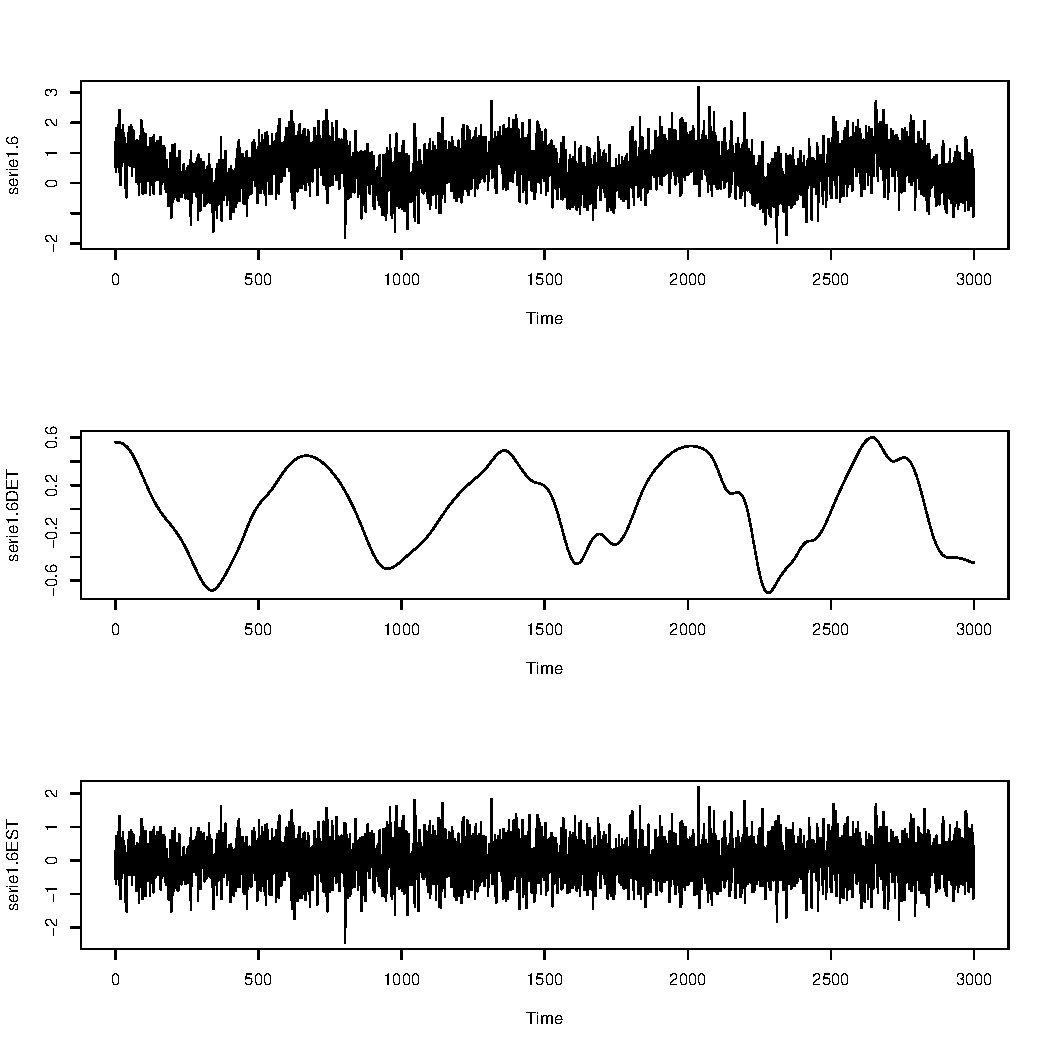
\includegraphics[scale=0.43]{serie1_6.pdf}
  \caption{Série 1.5 e Série 1.6}

\end{center}
\end{figure}

\graphicspath{{imagens/}}
\begin{figure}[H]
\begin{center}
  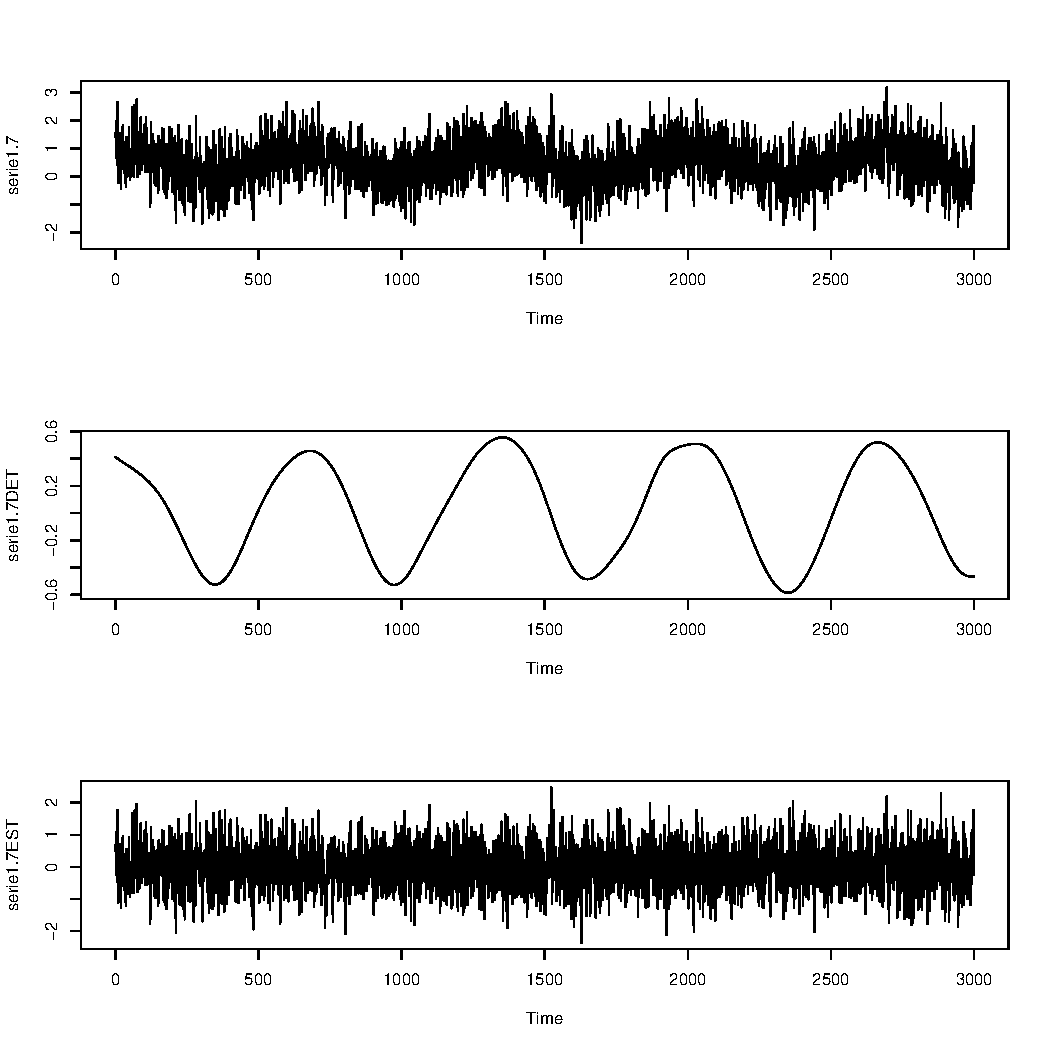
\includegraphics[scale=0.43]{serie1_7.pdf} \quad
  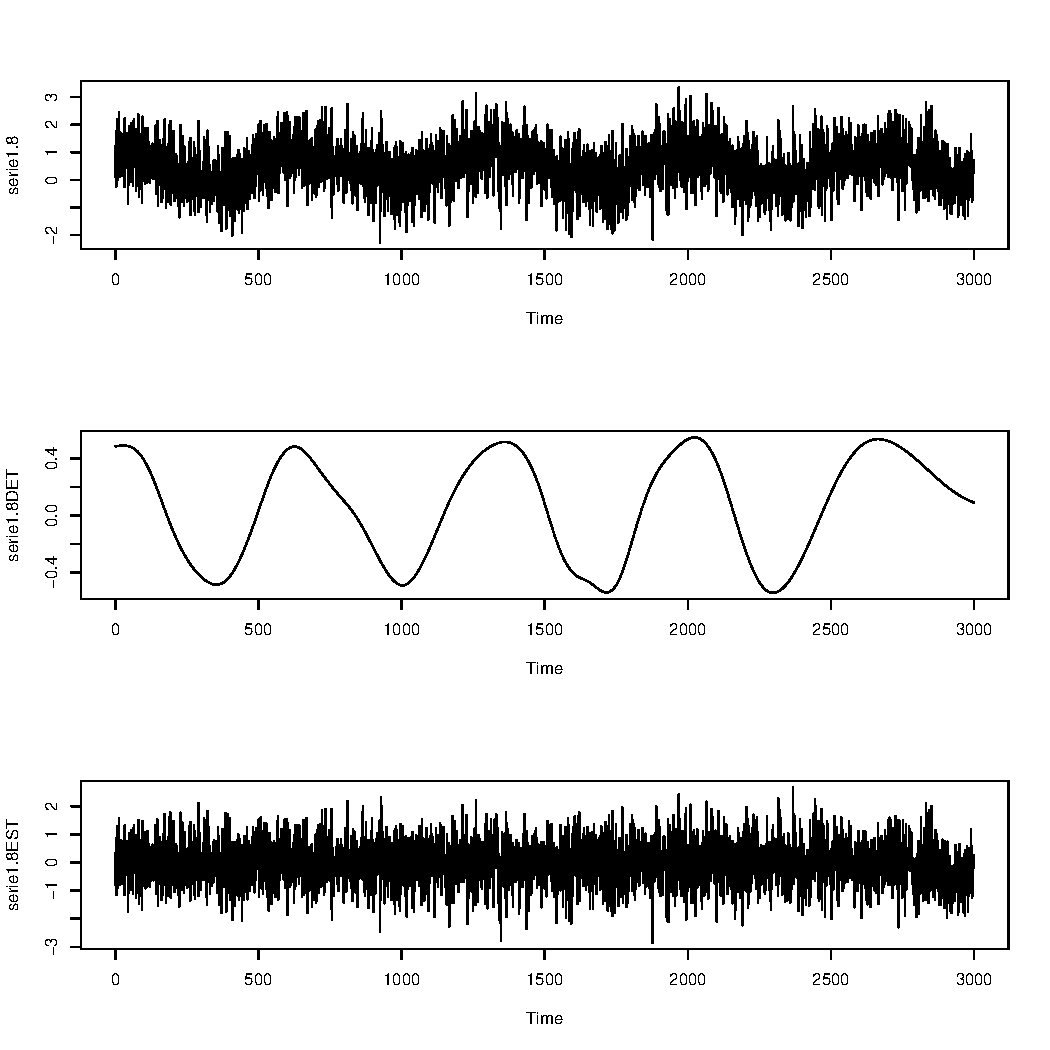
\includegraphics[scale=0.43]{serie1_8.pdf}
  \caption{Série 1.7 e Série 1.8}

\end{center}
\end{figure}

\graphicspath{{imagens/}}
\begin{figure}[H]
\begin{center}
  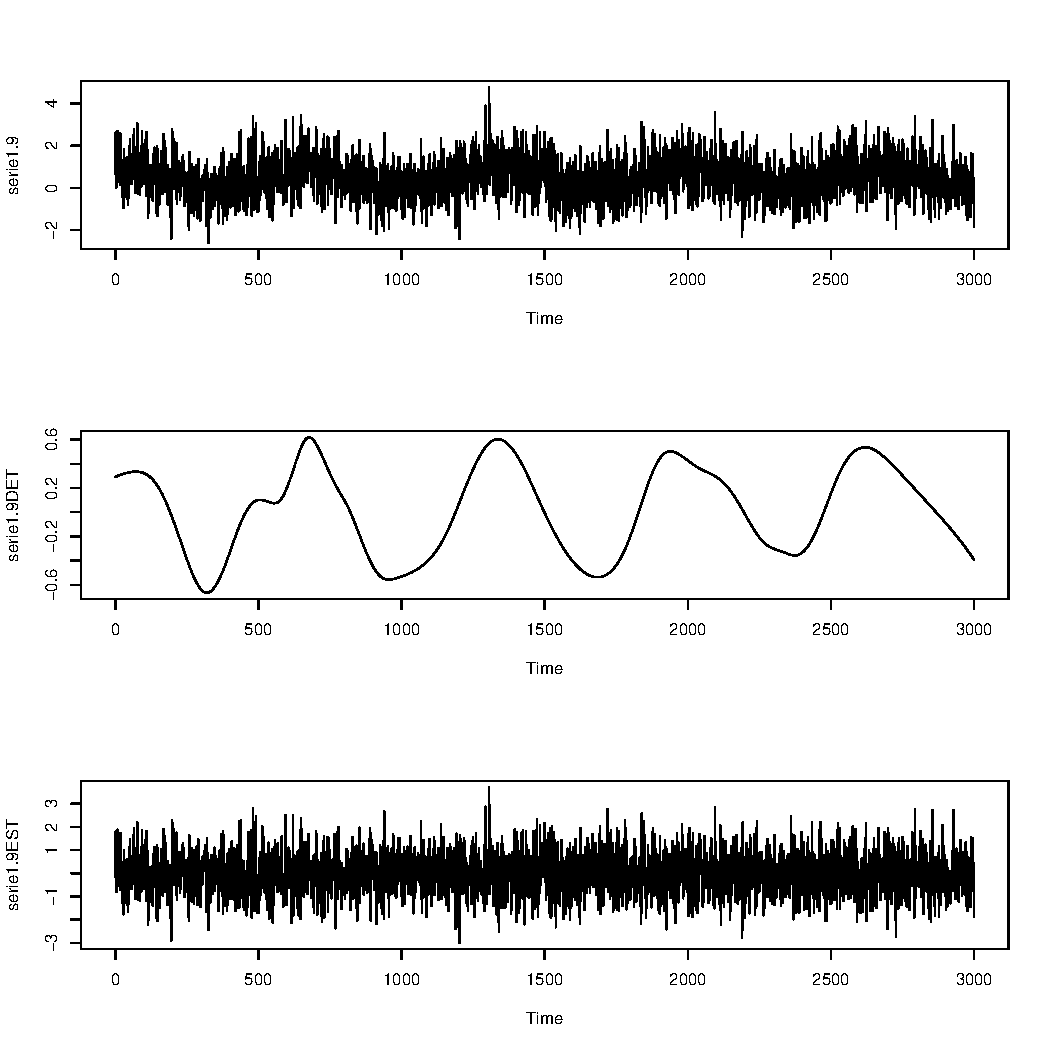
\includegraphics[scale=0.43]{serie1_9.pdf} \quad
  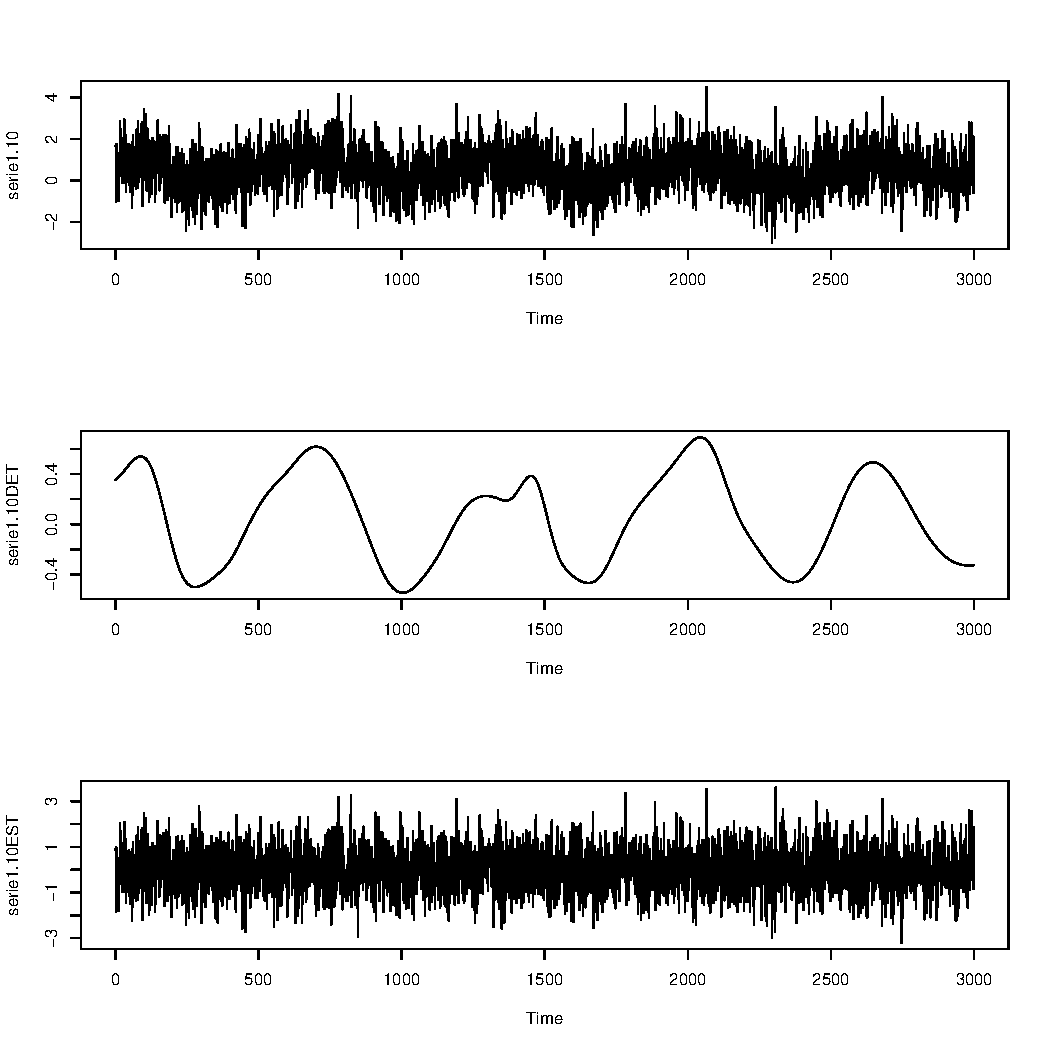
\includegraphics[scale=0.43]{serie1_10.pdf}
  \caption{Série 1.9 e Série 1.10}

\end{center}
\end{figure}

\section{Séries TIPO 2}
10 séries cossenoide com ruído ao longo da série e tendência.
\graphicspath{{imagens/}}
\begin{figure}[H]
\begin{center}
  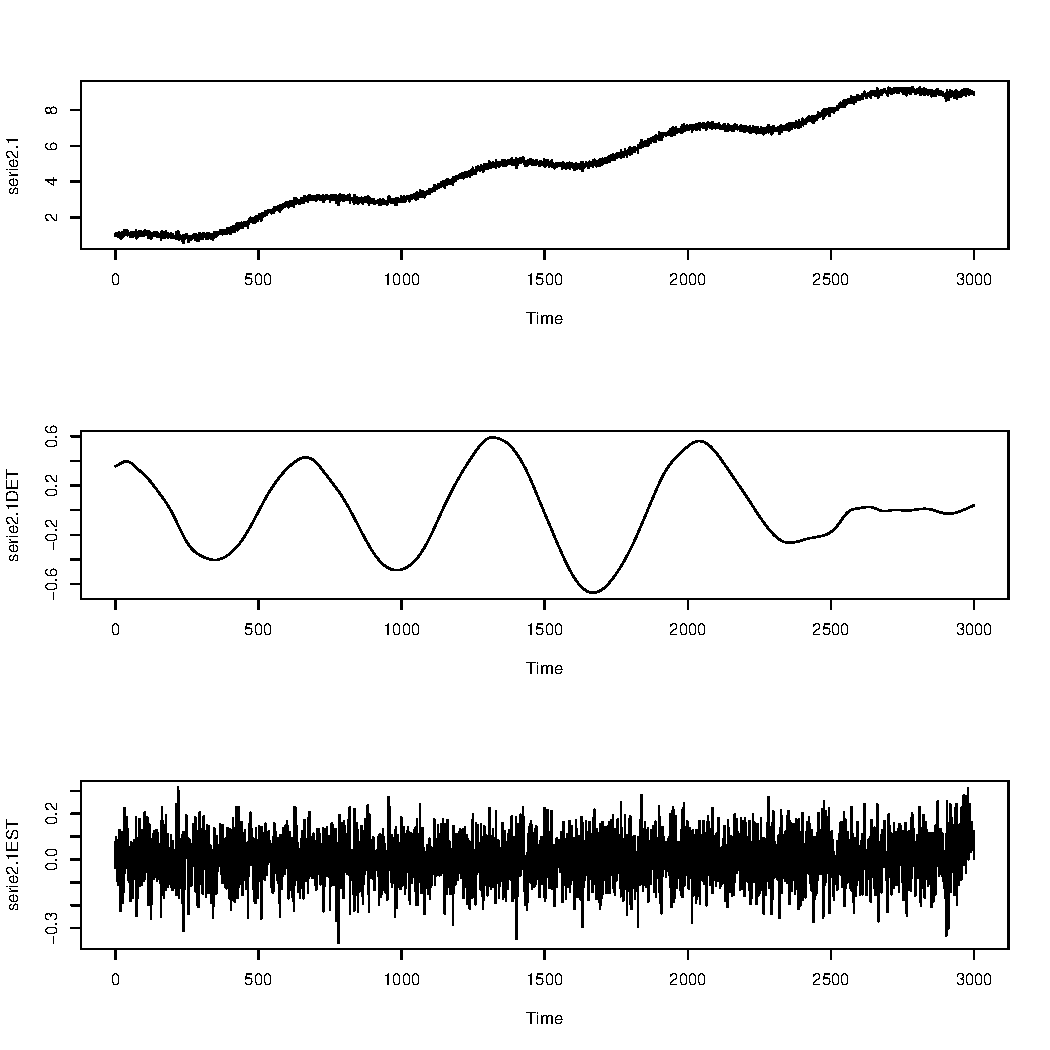
\includegraphics[scale=0.43]{serie2_1.pdf} \quad
  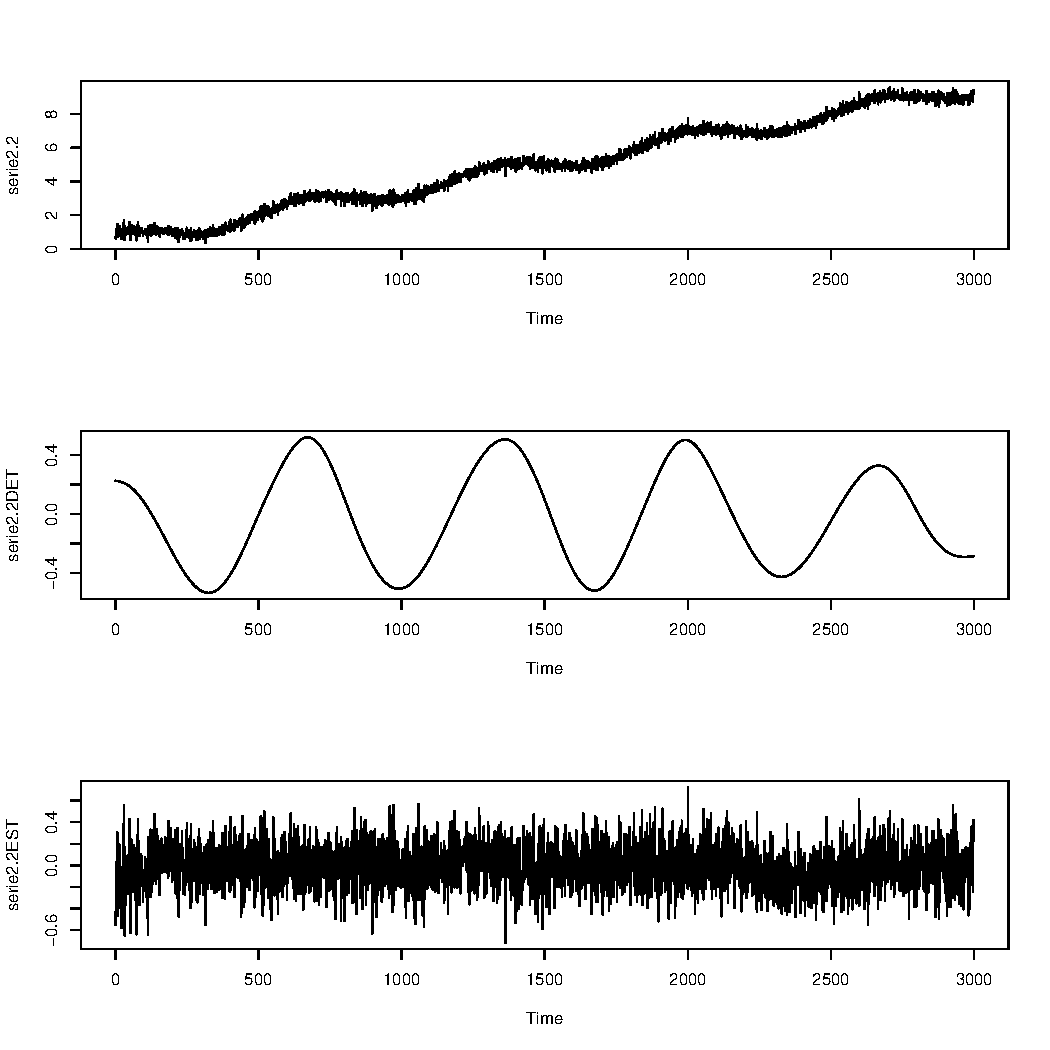
\includegraphics[scale=0.43]{serie2_2.pdf}
  \caption{Série 2.1 e Série 2.2}

\end{center}
\end{figure}

\graphicspath{{imagens/}}
\begin{figure}[H]
\begin{center}
  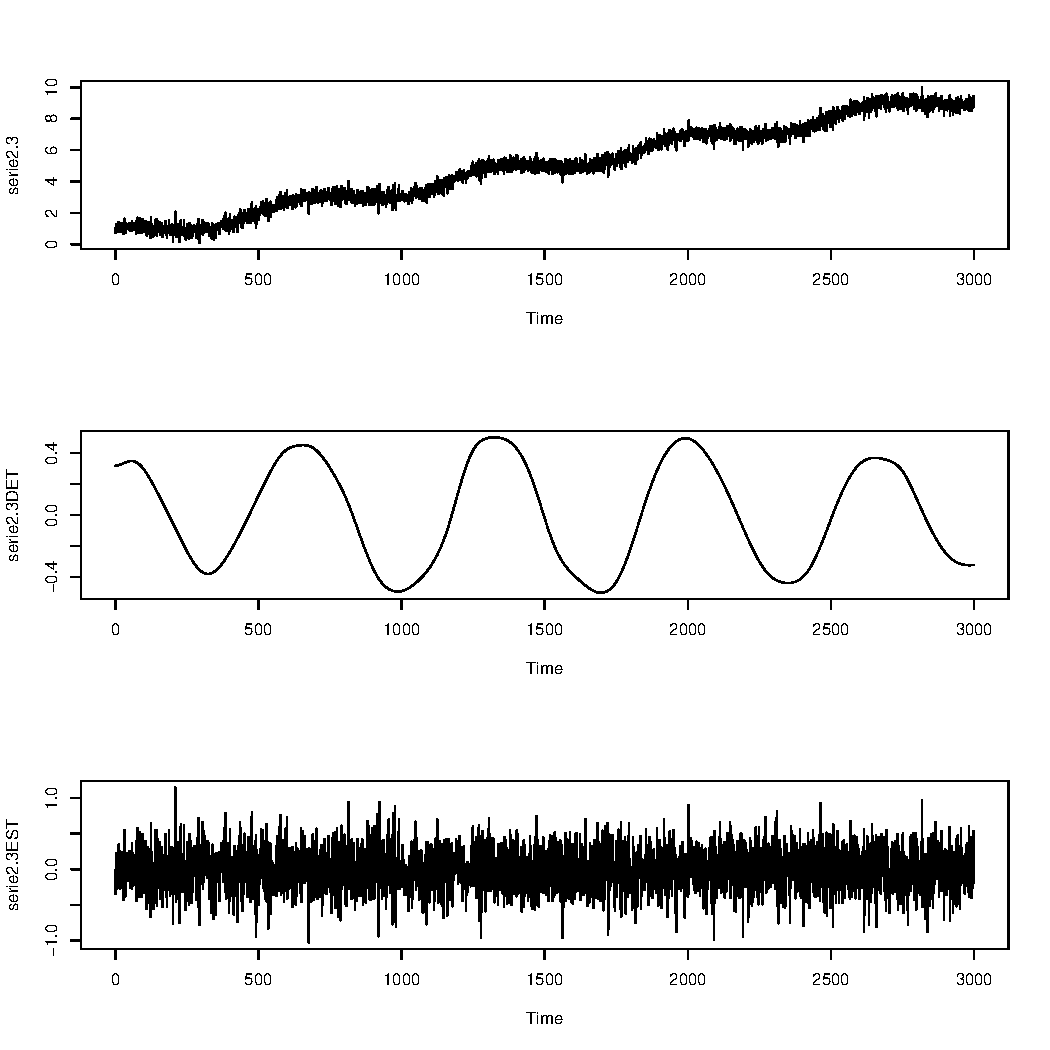
\includegraphics[scale=0.43]{serie2_3.pdf} \quad
  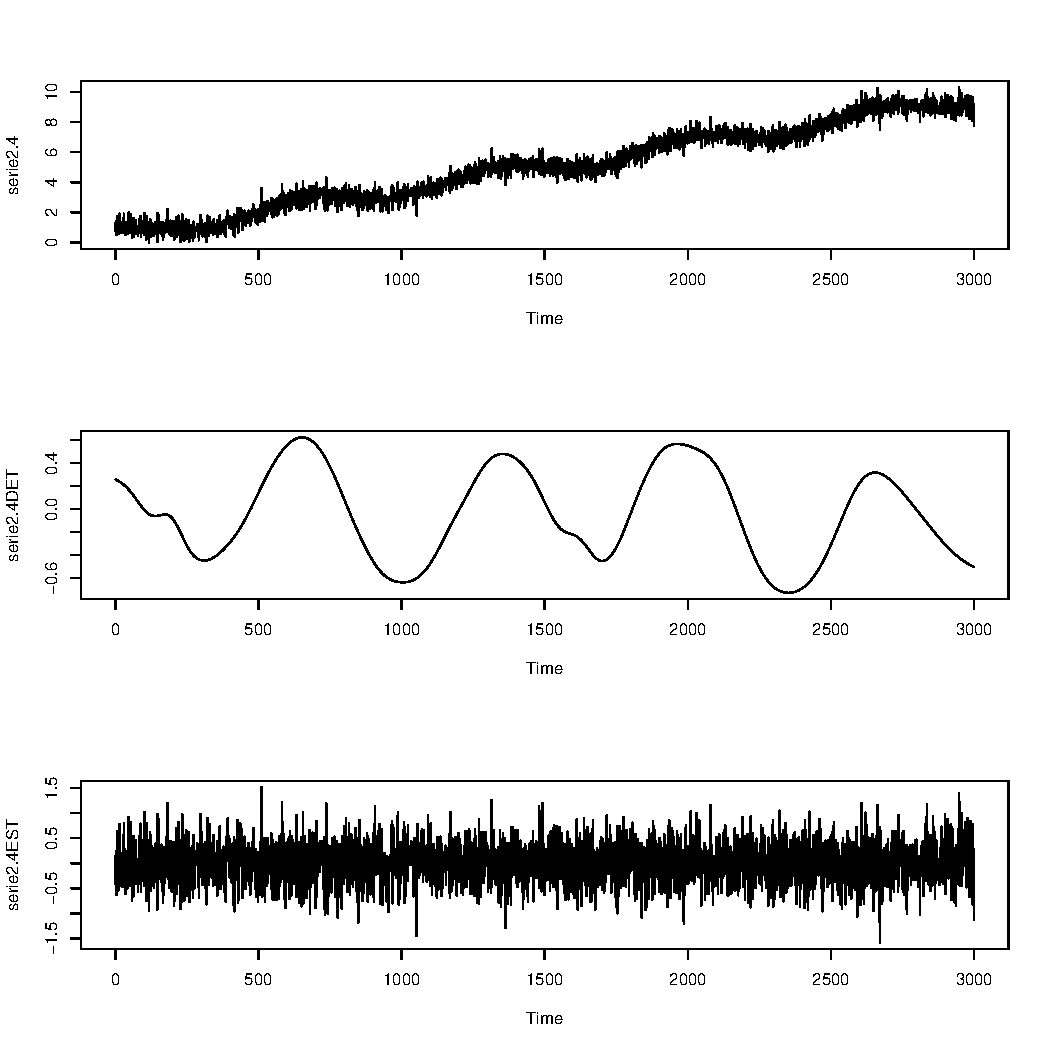
\includegraphics[scale=0.43]{serie2_4.pdf}
  \caption{Série 2.3 e Série 2.4}

\end{center}
\end{figure}

\graphicspath{{imagens/}}
\begin{figure}[H]
\begin{center}
  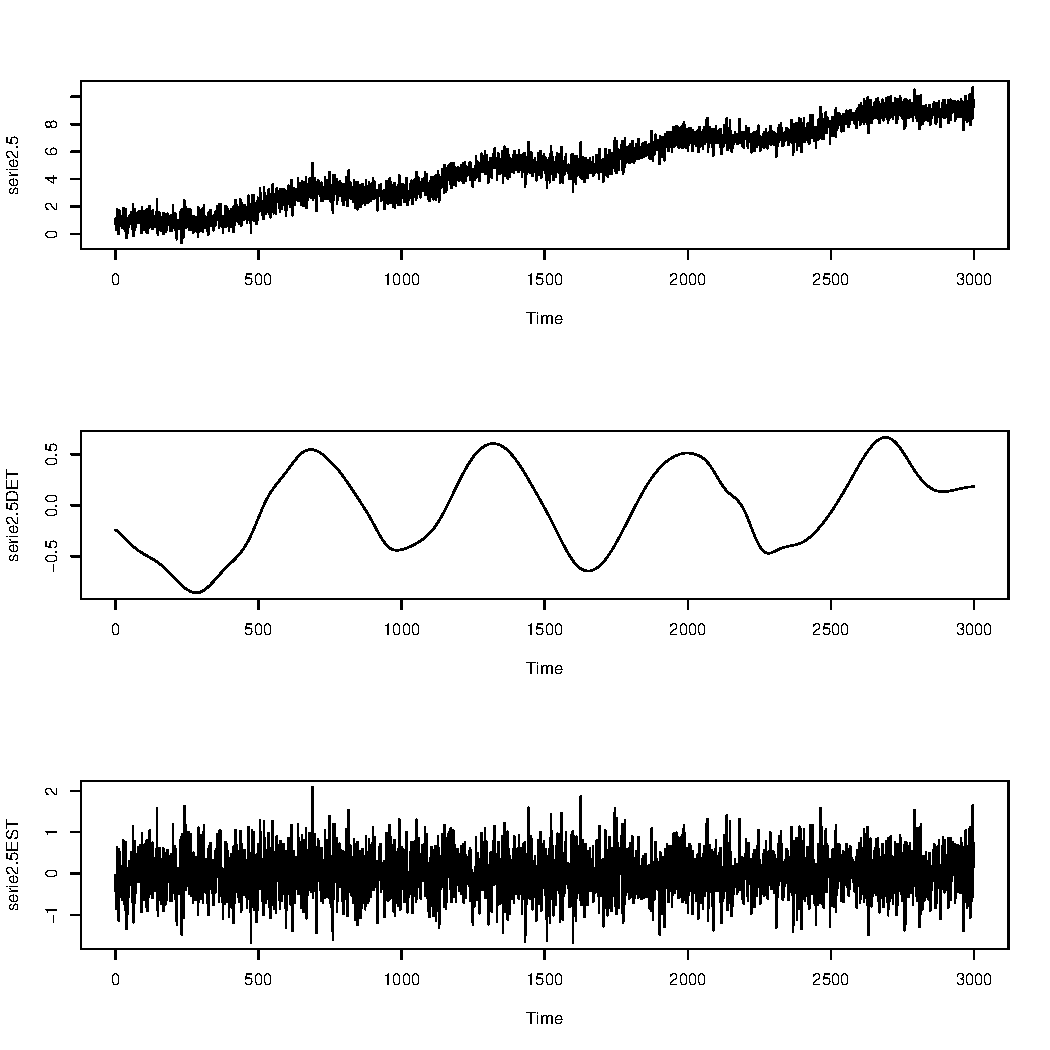
\includegraphics[scale=0.43]{serie2_5.pdf} \quad
  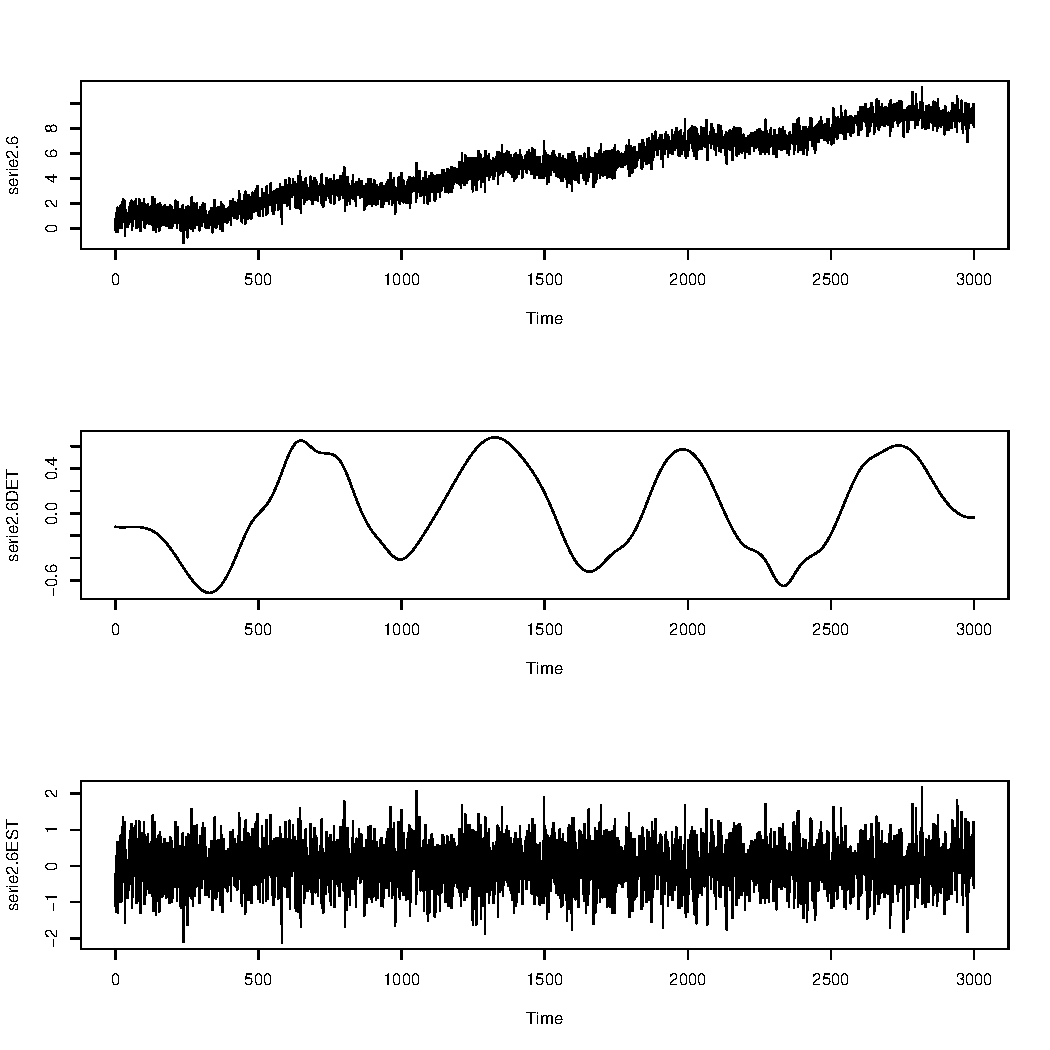
\includegraphics[scale=0.43]{serie2_6.pdf}
  \caption{Série 2.5 e Série 2.6}

\end{center}
\end{figure}

\graphicspath{{imagens/}}
\begin{figure}[H]
\begin{center}
  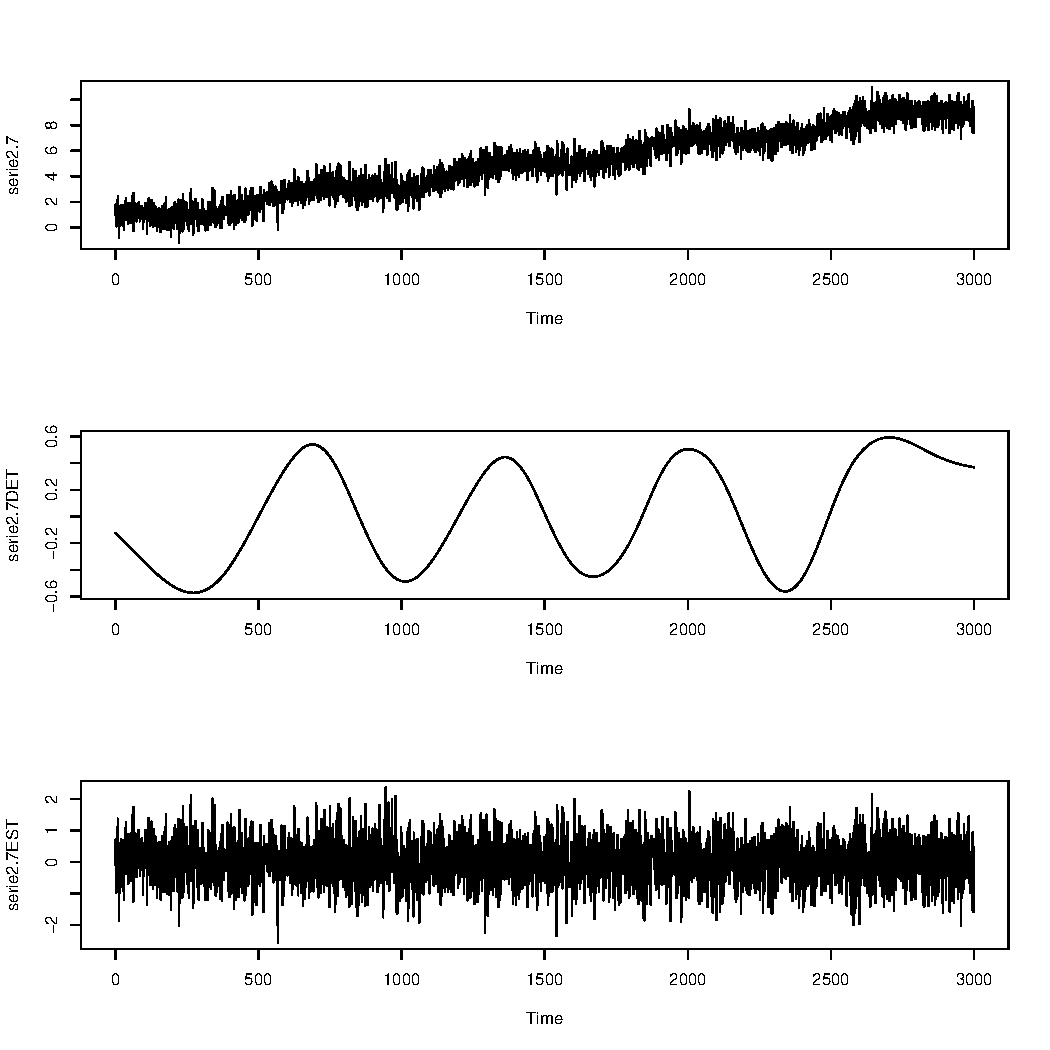
\includegraphics[scale=0.43]{serie2_7.pdf} \quad
  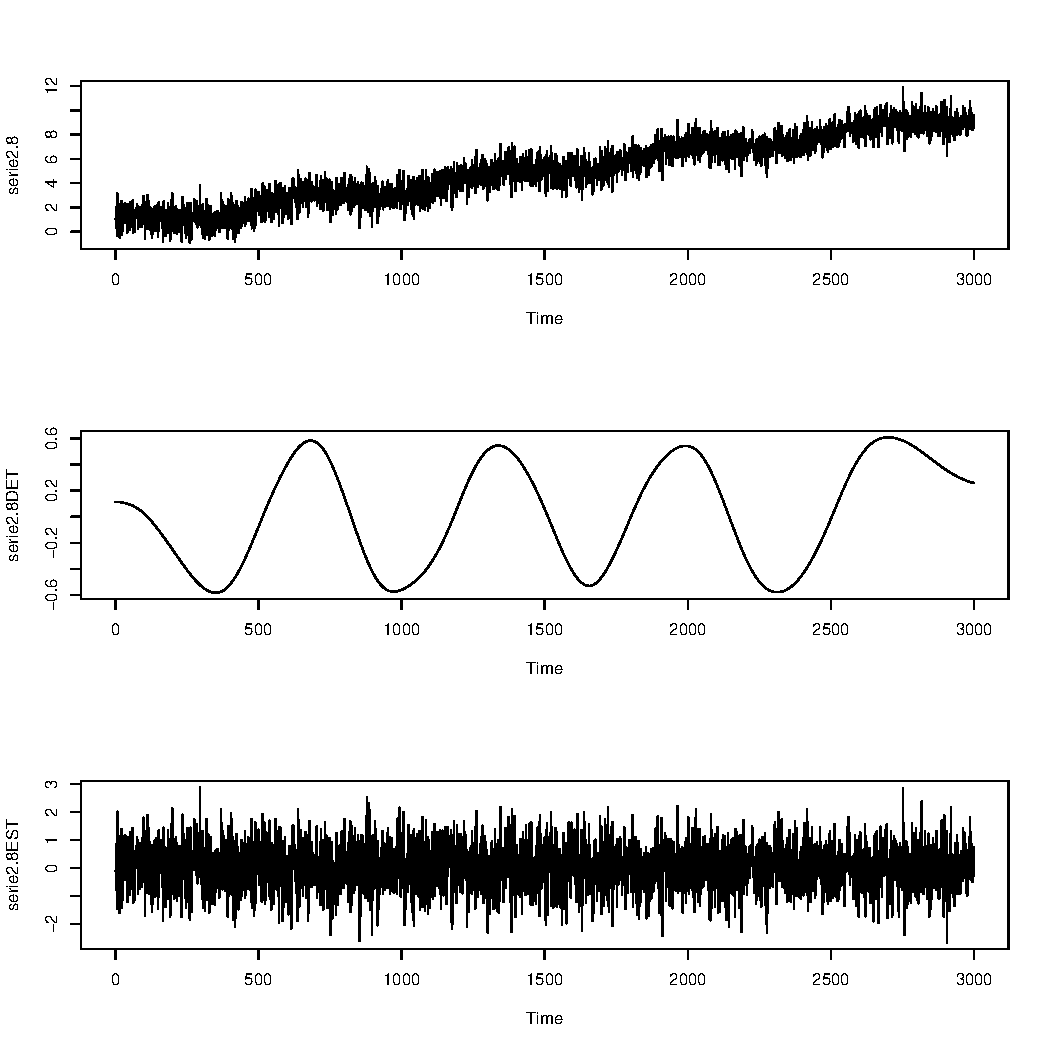
\includegraphics[scale=0.43]{serie2_8.pdf}
  \caption{Série 2.7 e Série 2.8}

\end{center}
\end{figure}

\graphicspath{{imagens/}}
\begin{figure}[H]
\begin{center}
  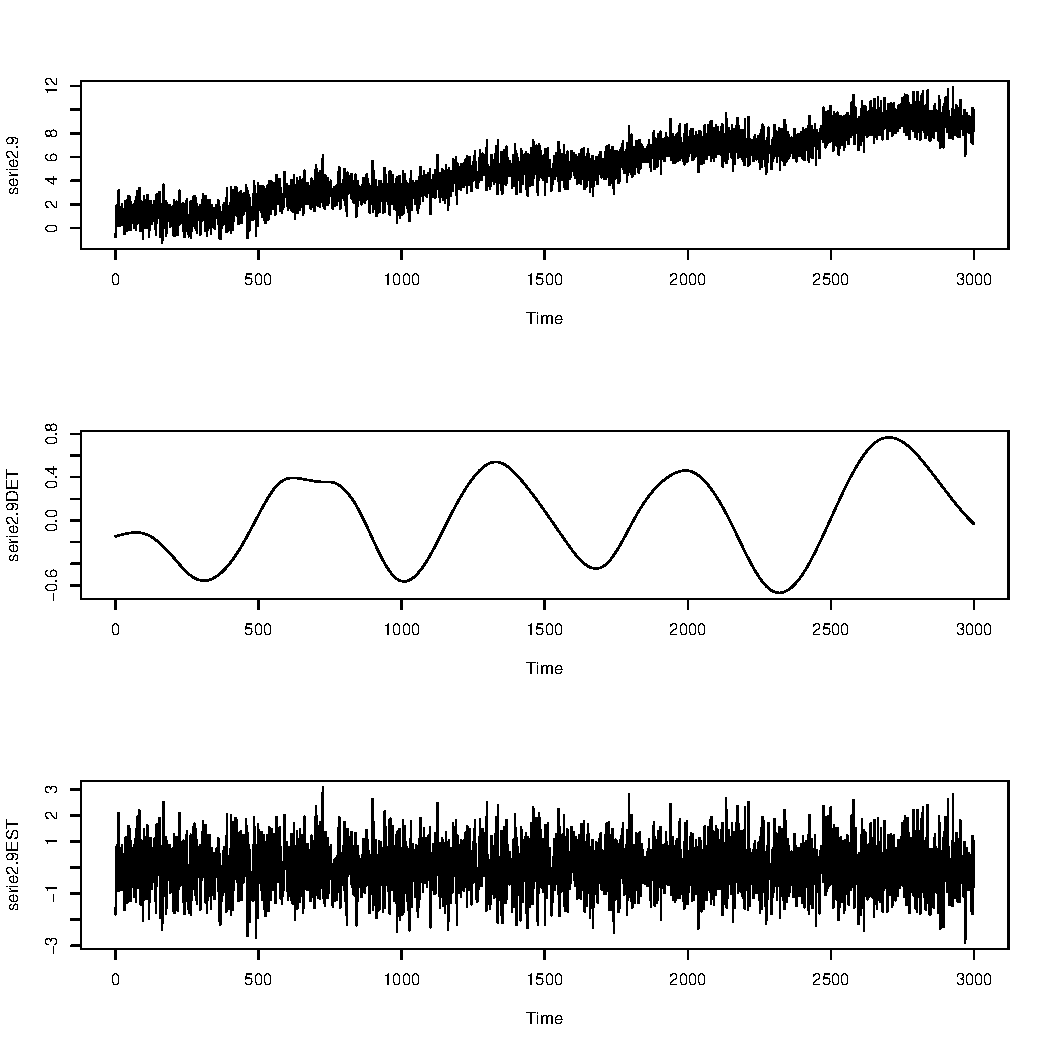
\includegraphics[scale=0.43]{serie2_9.pdf} \quad
  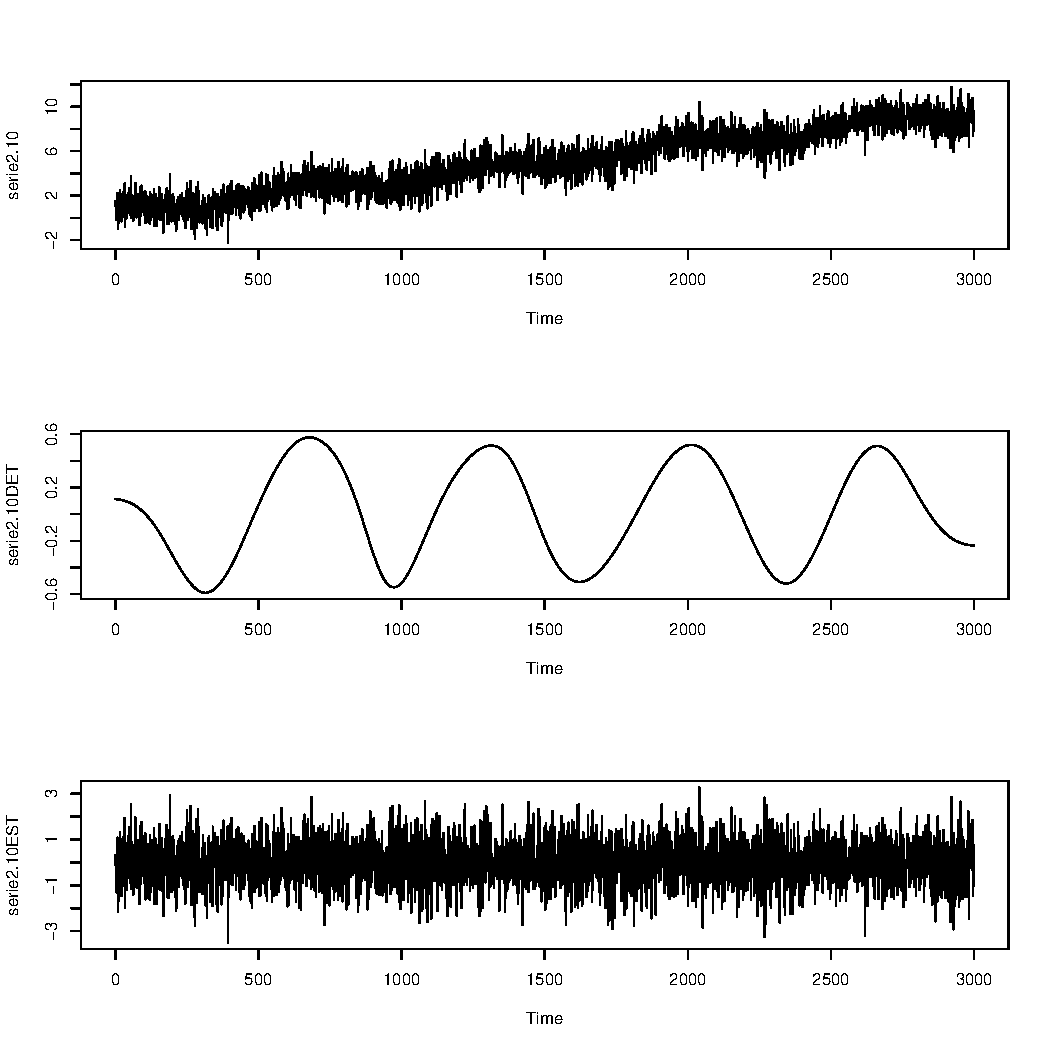
\includegraphics[scale=0.43]{serie2_10.pdf}
  \caption{Série 2.9 e Série 2.10}

\end{center}
\end{figure}

\section{Séries TIPO 3}
10 séries senoide com ruído ao longo da série.
\graphicspath{{imagens/}}
\begin{figure}[H]
\begin{center}
  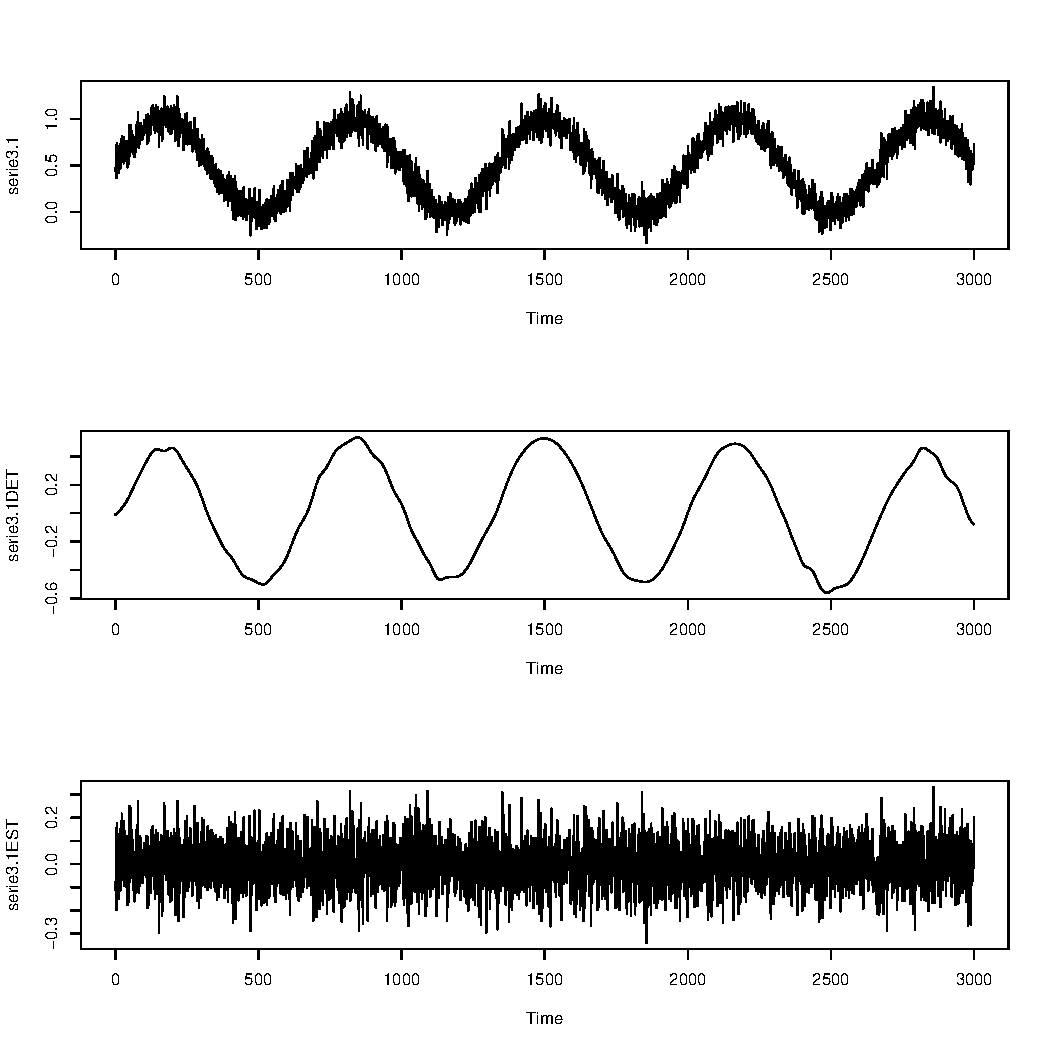
\includegraphics[scale=0.43]{serie3_1.pdf} \quad
  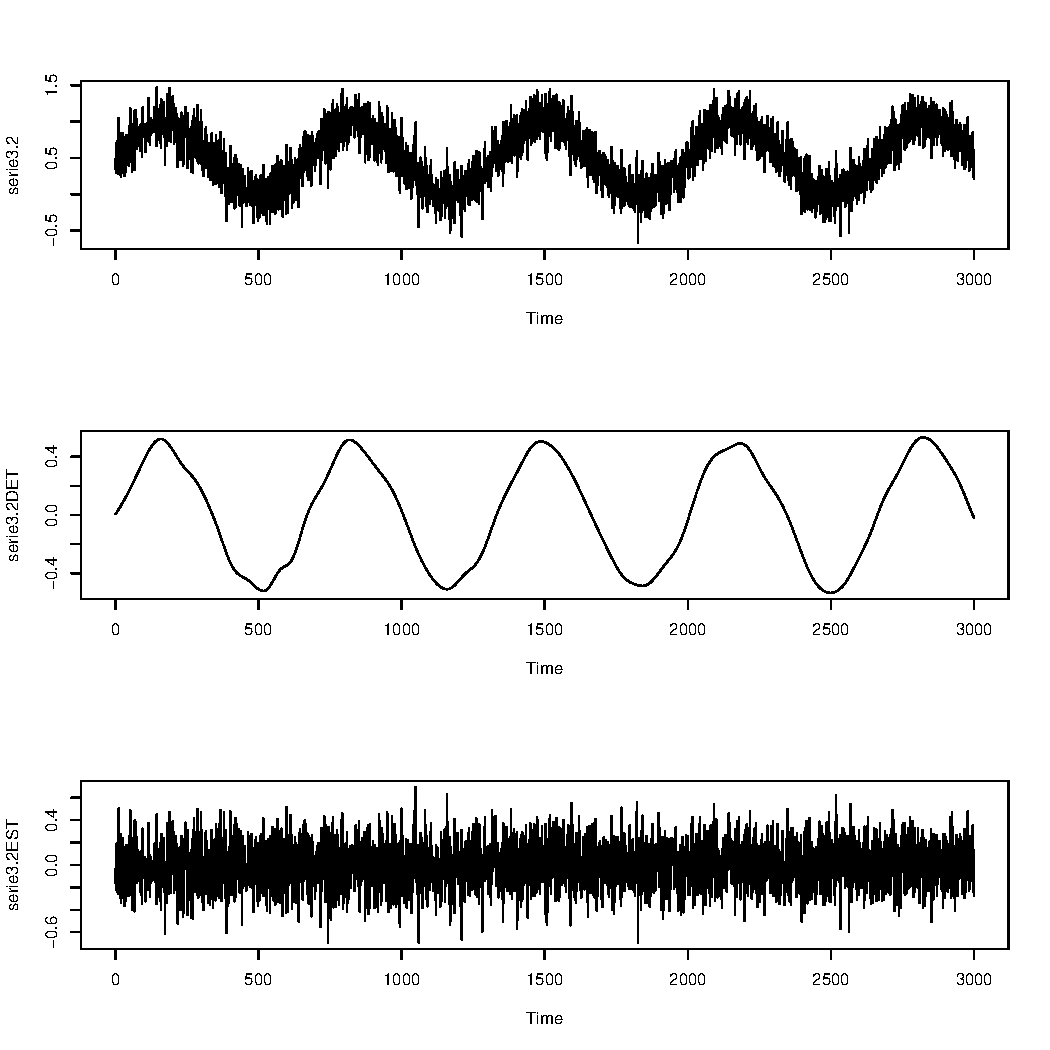
\includegraphics[scale=0.43]{serie3_2.pdf}
  \caption{Série 3.1 e Série 3.2}

\end{center}
\end{figure}

\graphicspath{{imagens/}}
\begin{figure}[H]
\begin{center}
  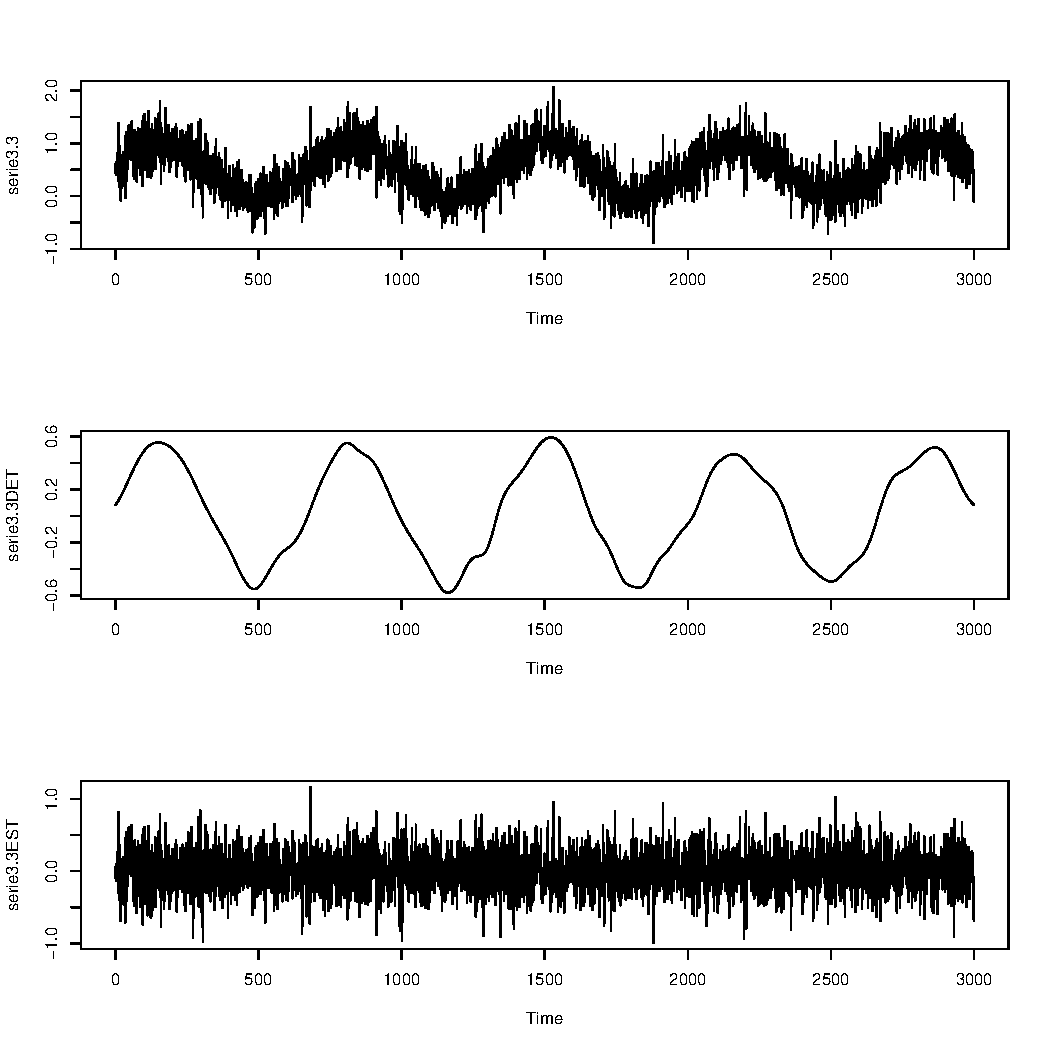
\includegraphics[scale=0.43]{serie3_3.pdf} \quad
  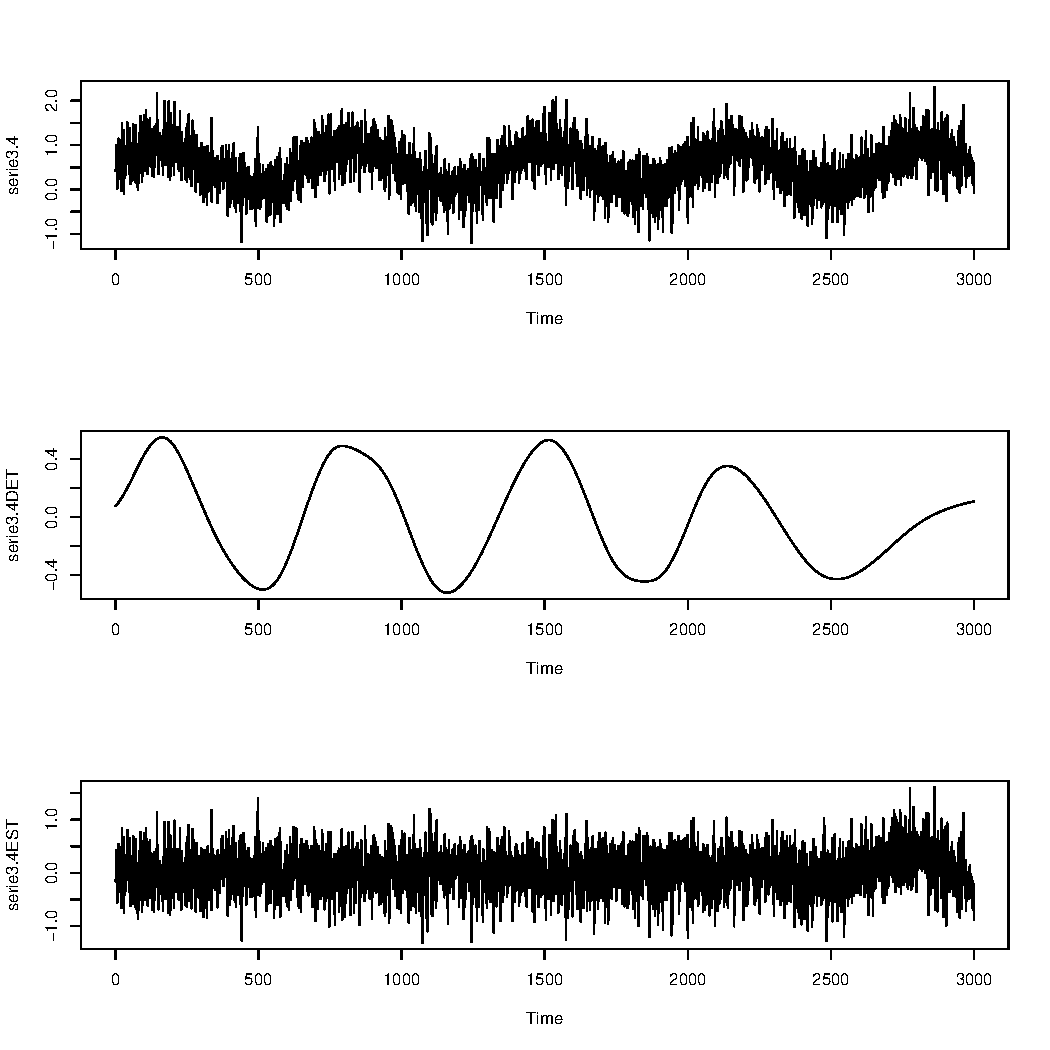
\includegraphics[scale=0.43]{serie3_4.pdf}
  \caption{Série 3.3 e Série 3.4}

\end{center}
\end{figure}

\graphicspath{{imagens/}}
\begin{figure}[H]
\begin{center}
  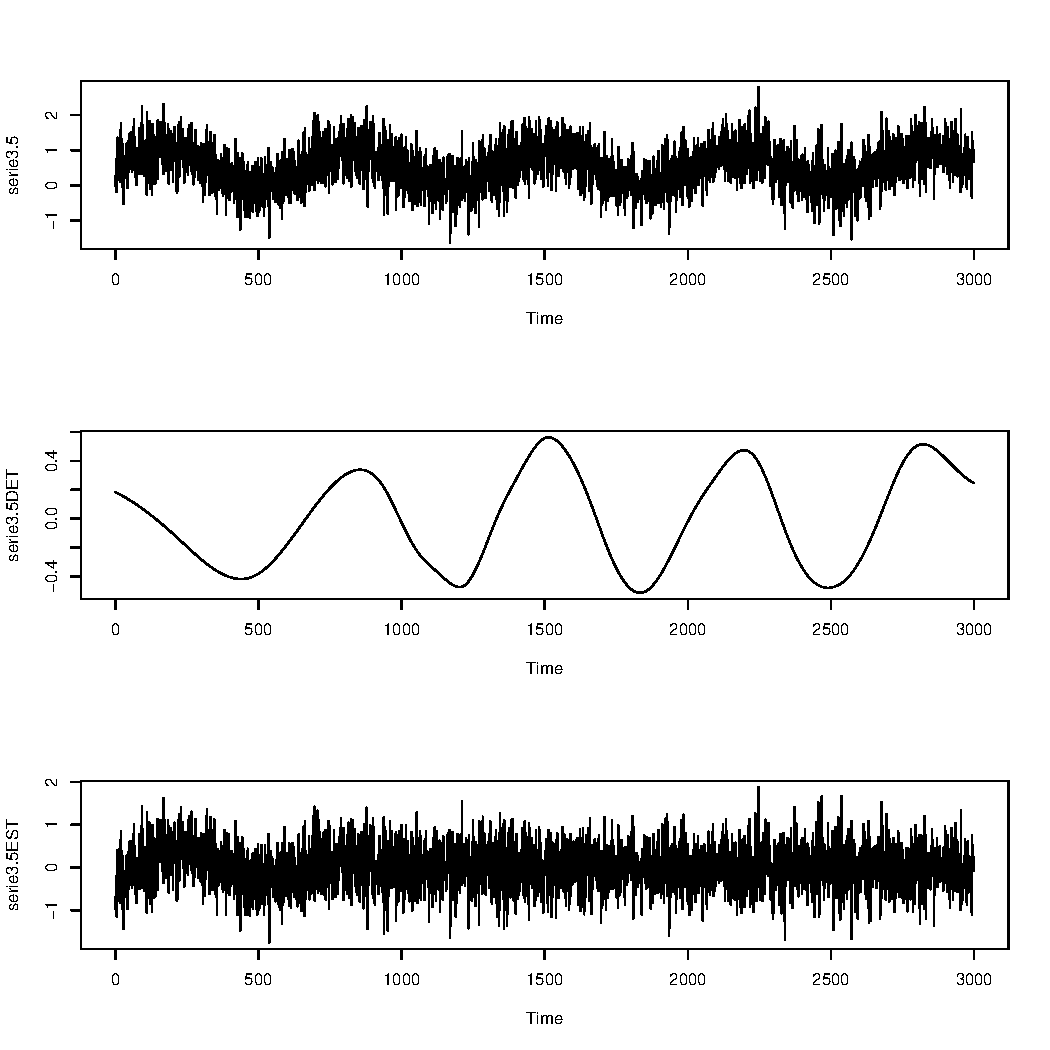
\includegraphics[scale=0.43]{serie3_5.pdf} \quad
  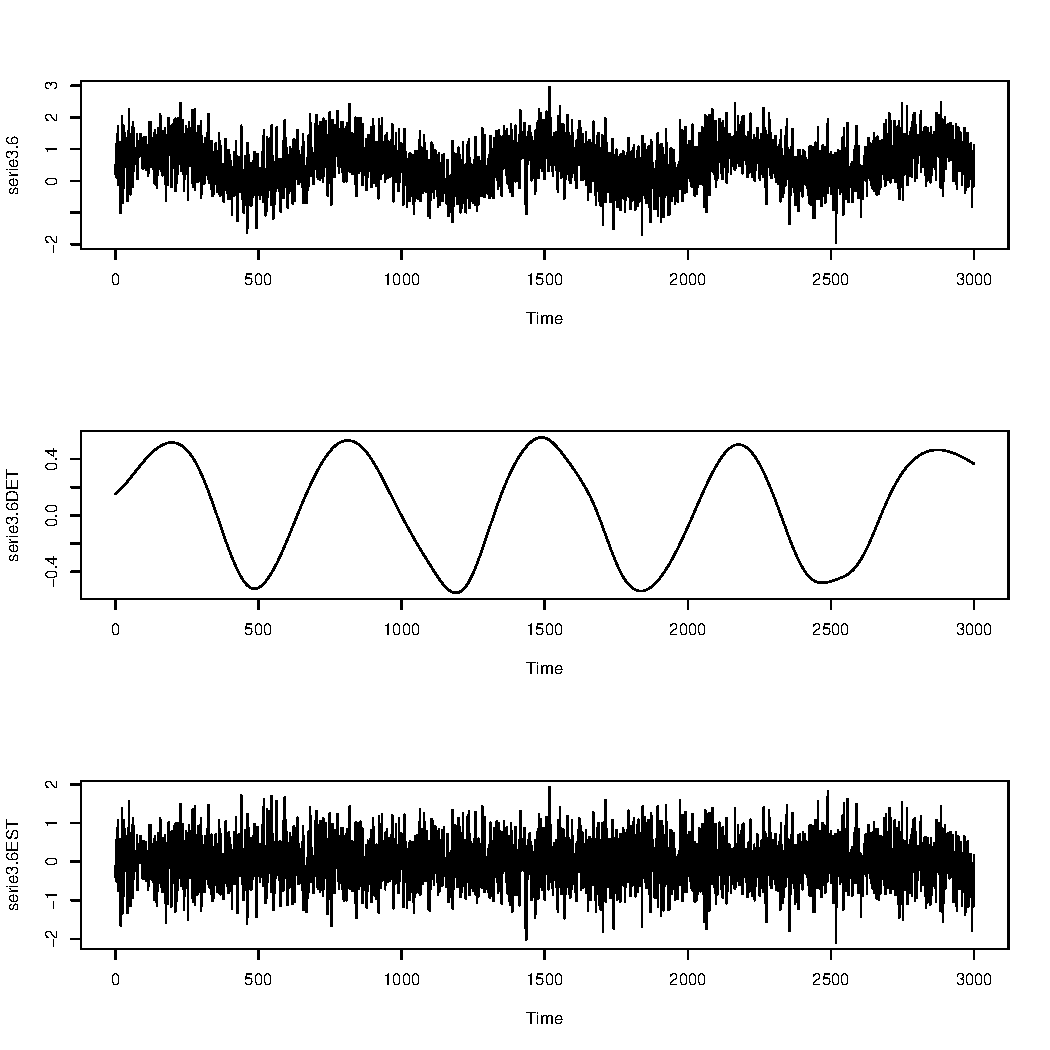
\includegraphics[scale=0.43]{serie3_6.pdf}
  \caption{Série 3.5 e Série 3.6}

\end{center}
\end{figure}

\graphicspath{{imagens/}}
\begin{figure}[H]
\begin{center}
  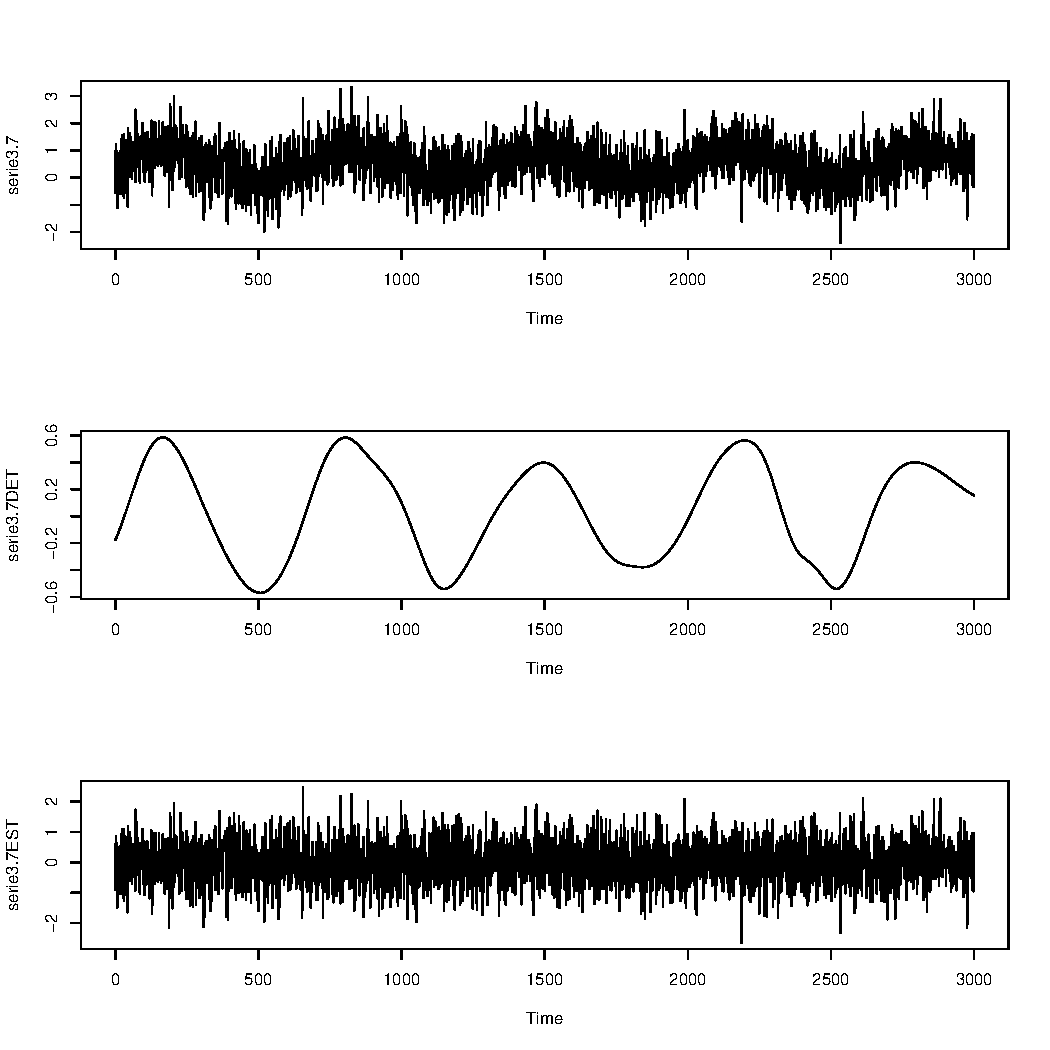
\includegraphics[scale=0.43]{serie3_7.pdf} \quad
  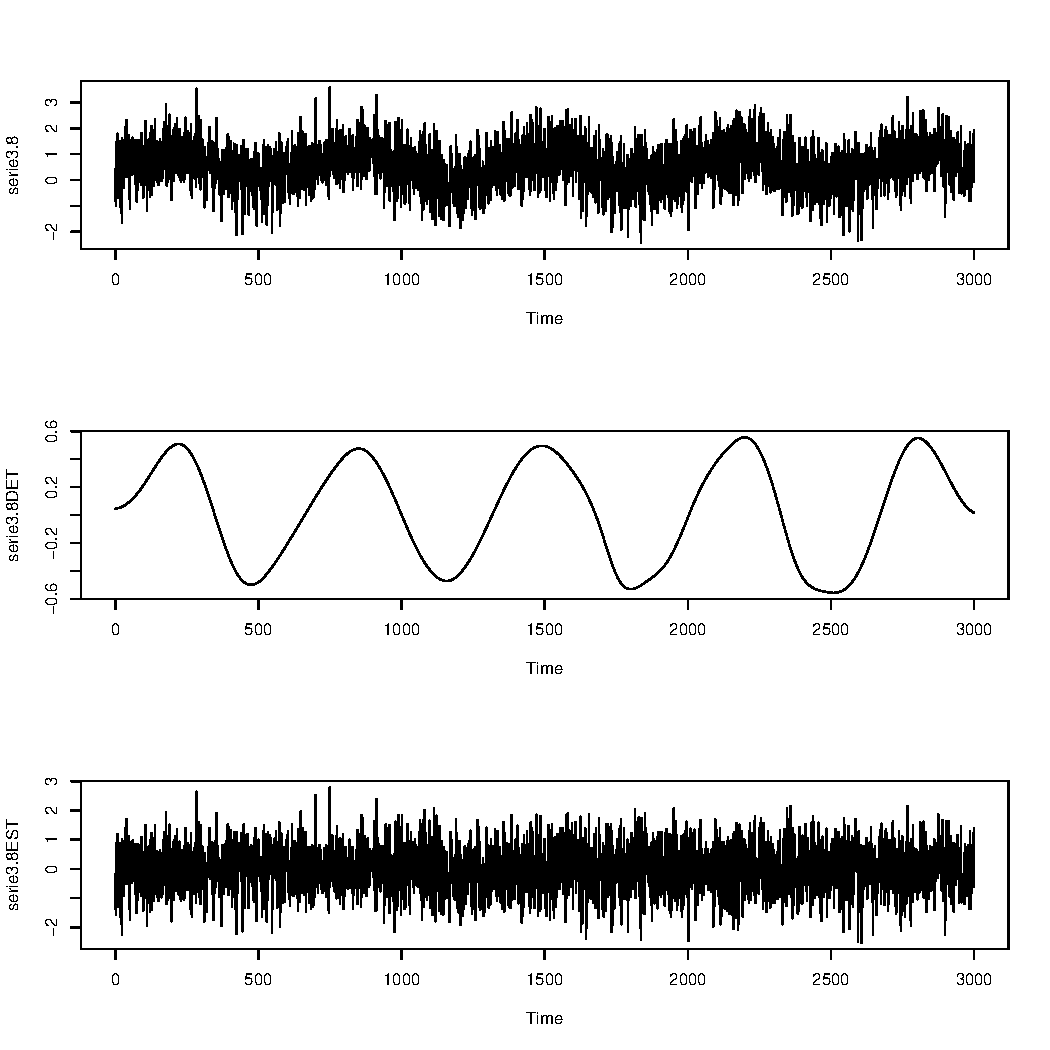
\includegraphics[scale=0.43]{serie3_8.pdf}
  \caption{Série 3.7 e Série 3.8}

\end{center}
\end{figure}

\graphicspath{{imagens/}}
\begin{figure}[H]
\begin{center}
  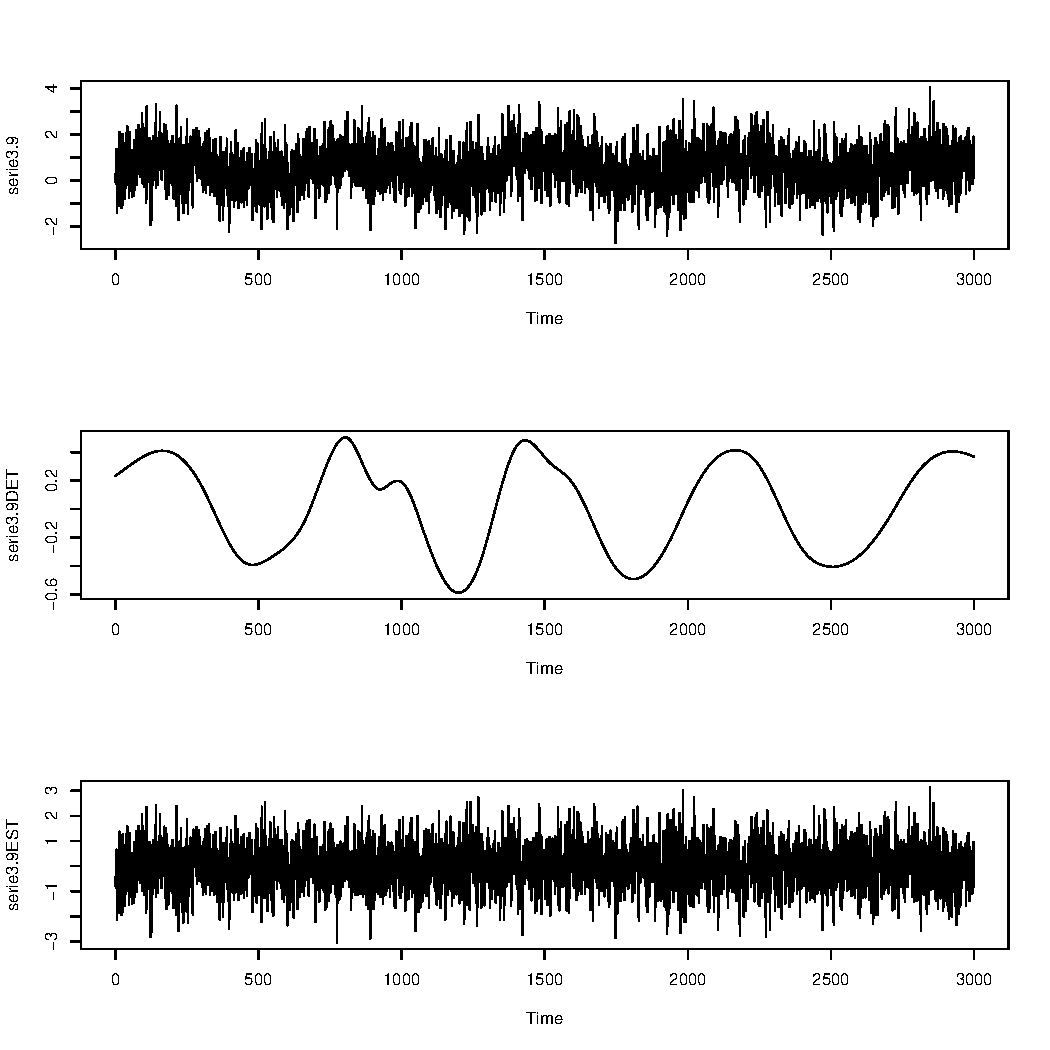
\includegraphics[scale=0.43]{serie3_9.pdf} \quad
  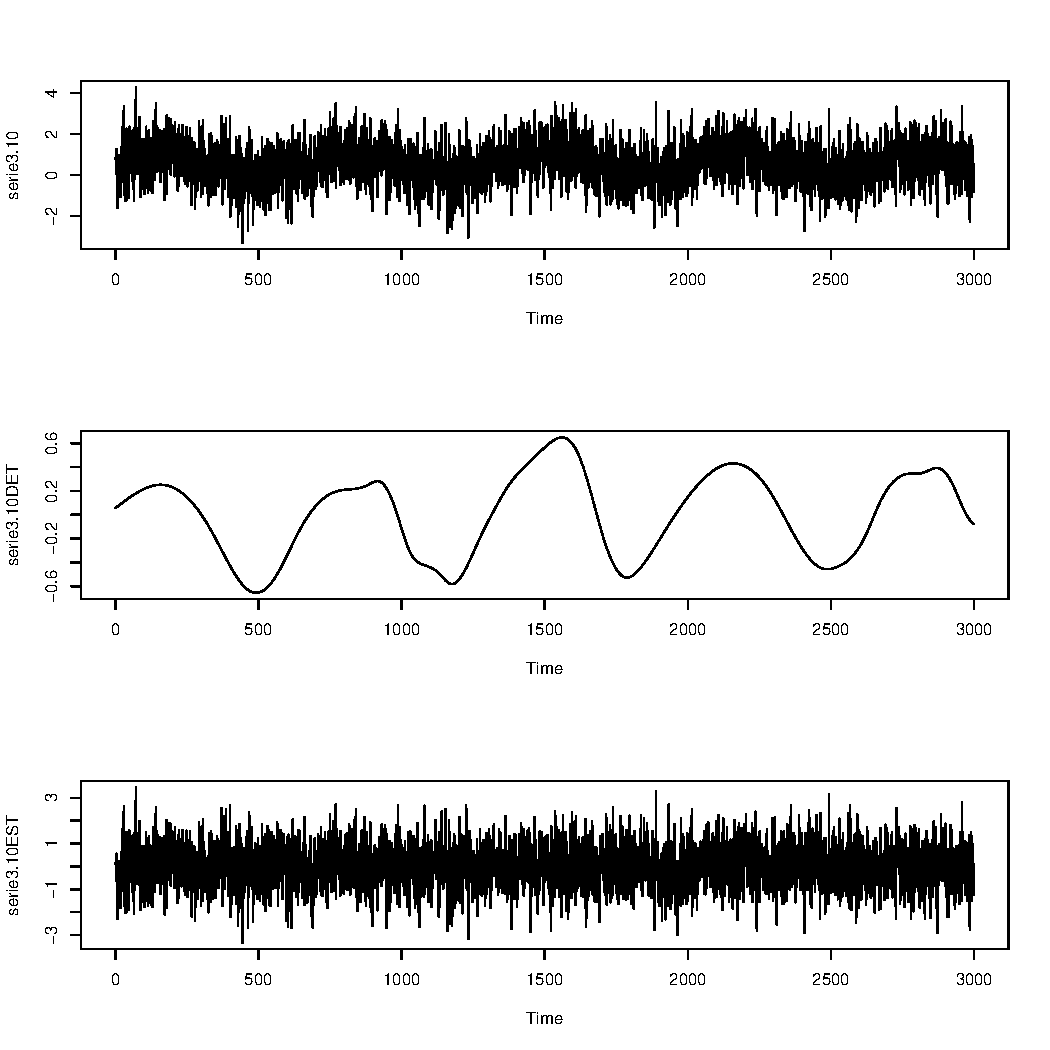
\includegraphics[scale=0.43]{serie3_10.pdf}
  \caption{Série 3.9 e Série 3.10}

\end{center}
\end{figure}

\section{Séries TIPO 4}
10 séries senoide com ruído ao longo da série e tendência.
\graphicspath{{imagens/}}
\begin{figure}[H]
\begin{center}
  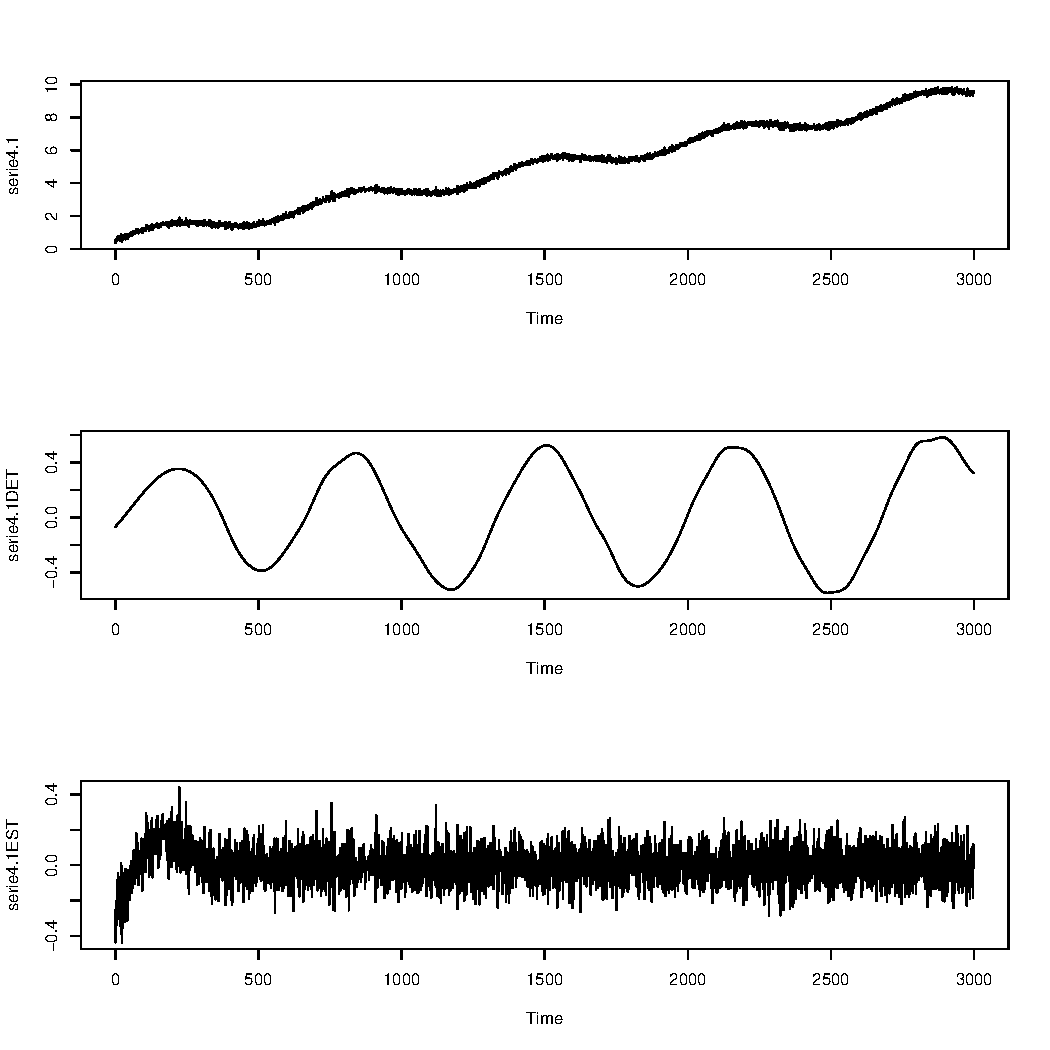
\includegraphics[scale=0.43]{serie4_1.pdf} \quad
  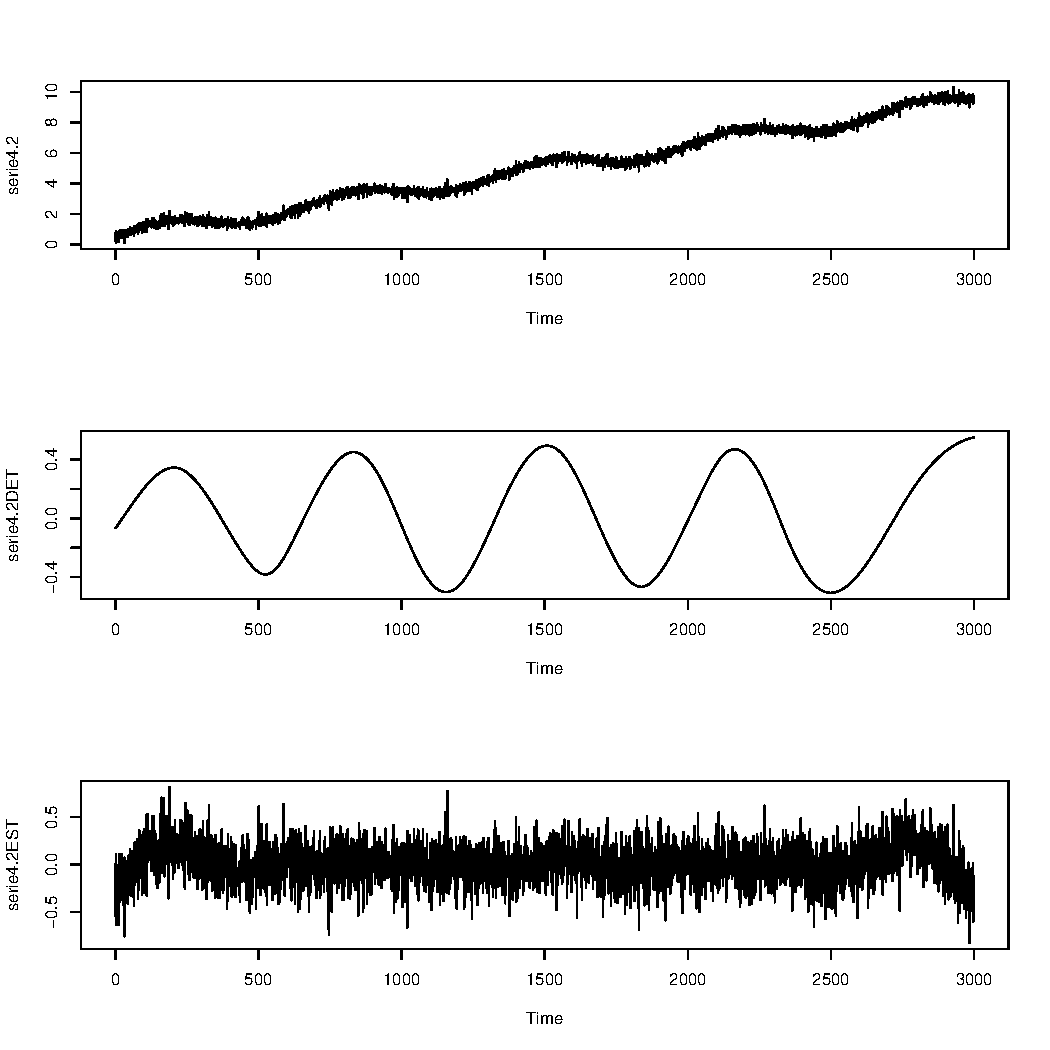
\includegraphics[scale=0.43]{serie4_2.pdf}
  \caption{Série 4.1 e Série 4.2}
\end{center}
\end{figure}

\graphicspath{{imagens/}}
\begin{figure}[H]
\begin{center}
  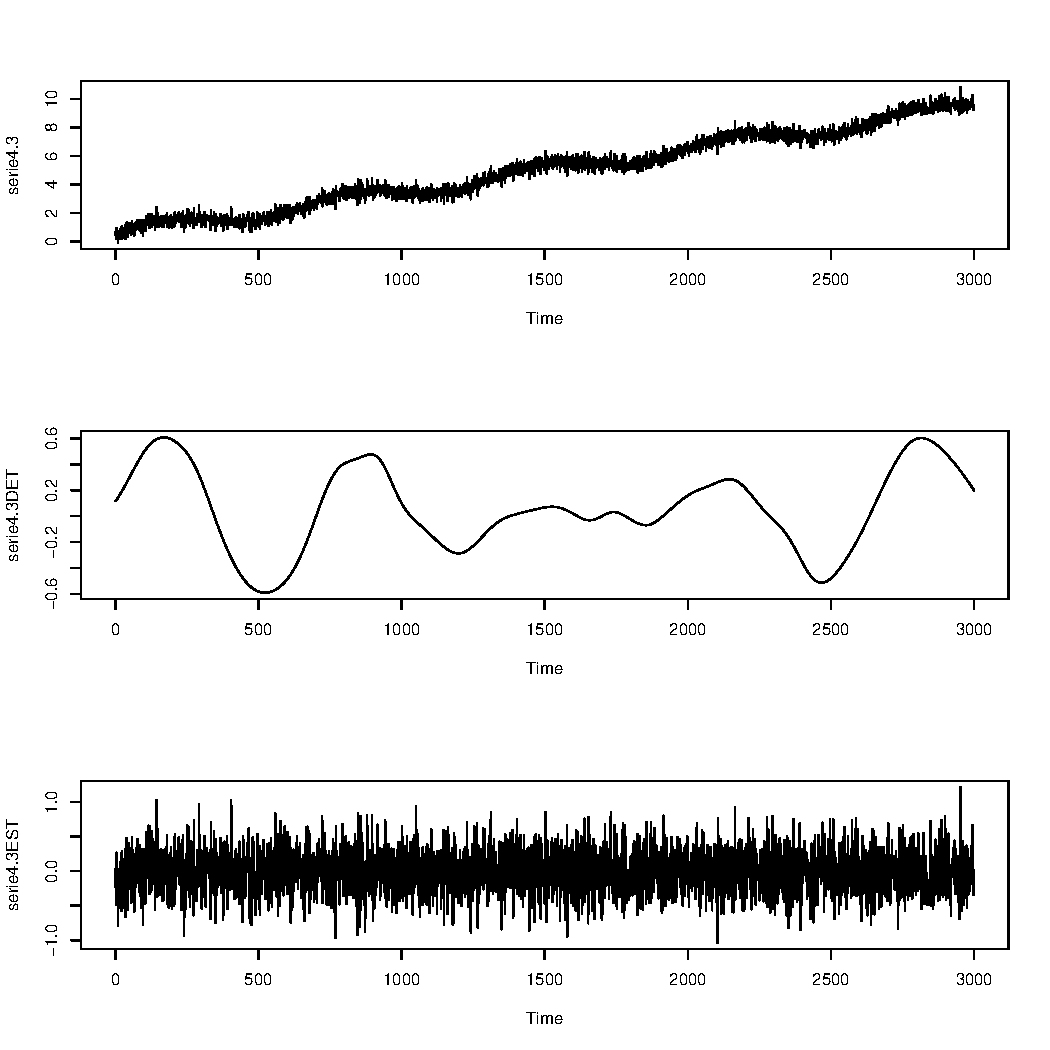
\includegraphics[scale=0.43]{serie4_3.pdf} \quad
 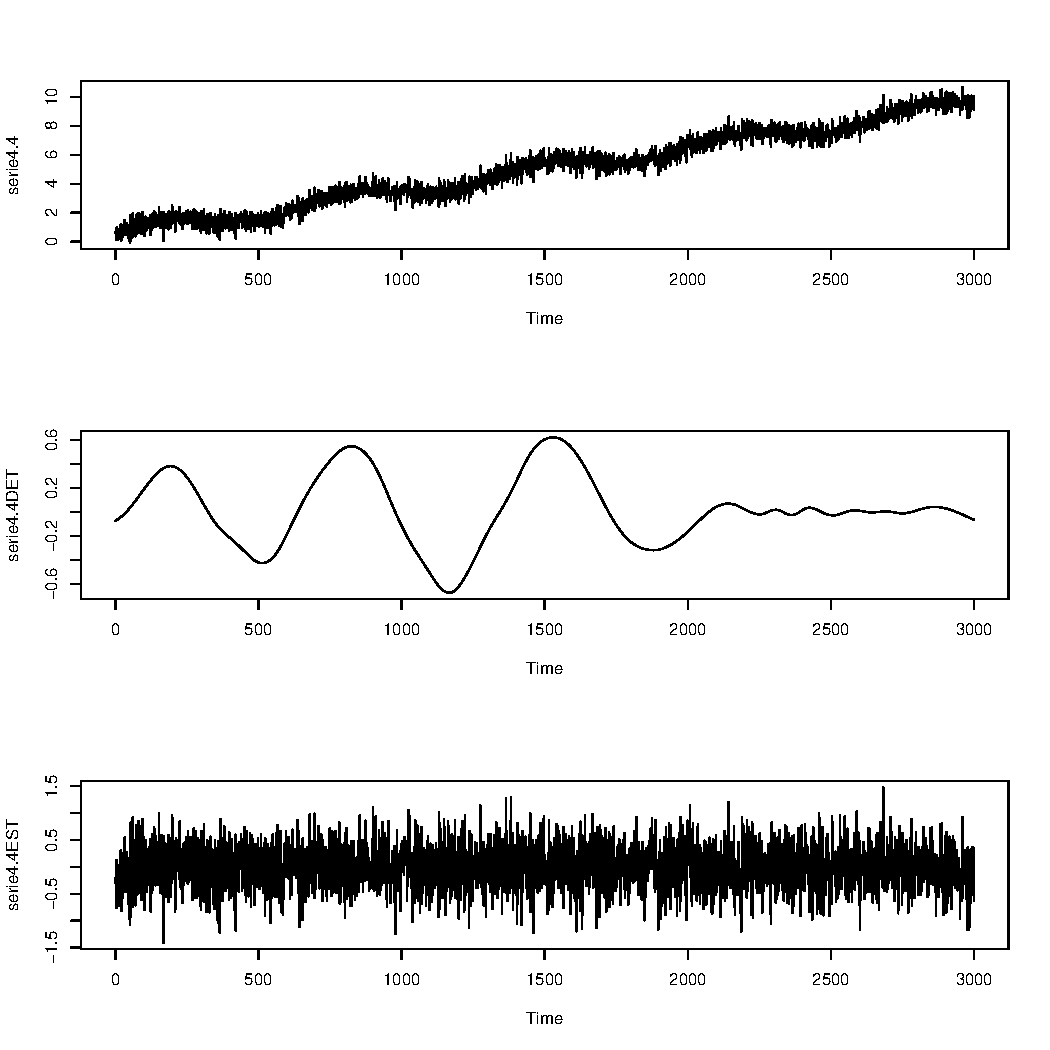
\includegraphics[scale=0.43]{serie4_4.pdf}
 \caption{Série 4.3 e Série 4.4}

\end{center}
\end{figure}

\graphicspath{{imagens/}}
\begin{figure}[H]
\begin{center}
  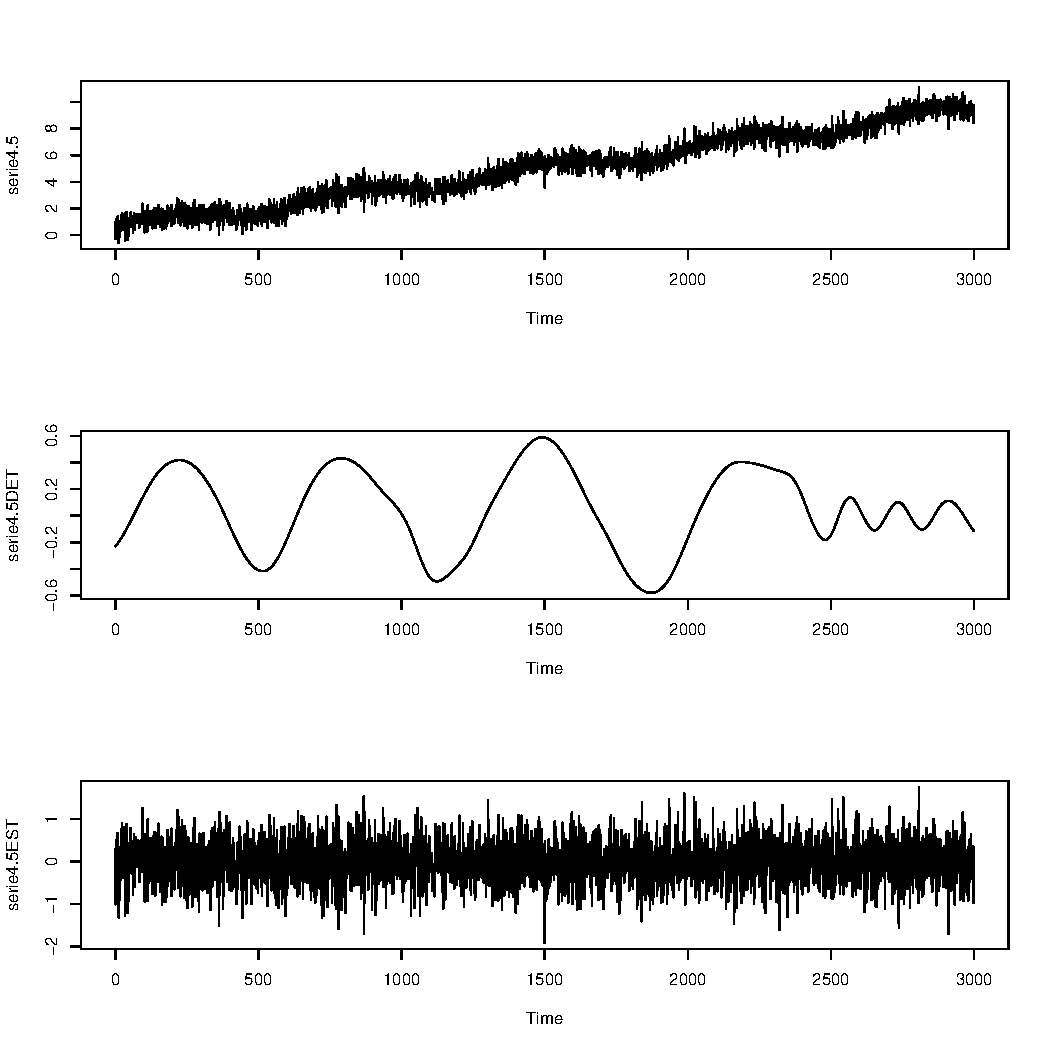
\includegraphics[scale=0.43]{serie4_5.pdf} \quad
  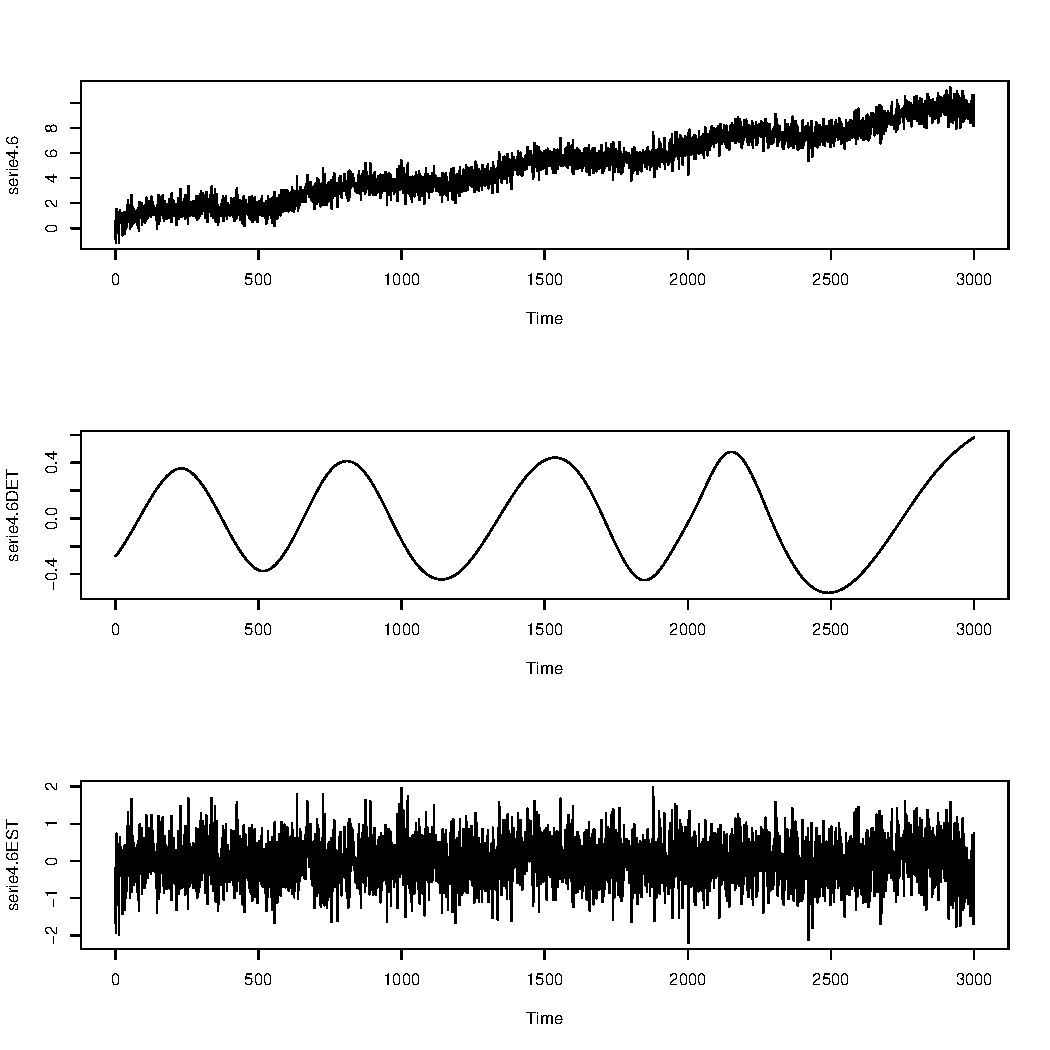
\includegraphics[scale=0.43]{serie4_6.pdf}
 \caption{Série 4.5 e Série 4.6}

\end{center}
\end{figure}

\graphicspath{{imagens/}}
\begin{figure}[H]
\begin{center}
  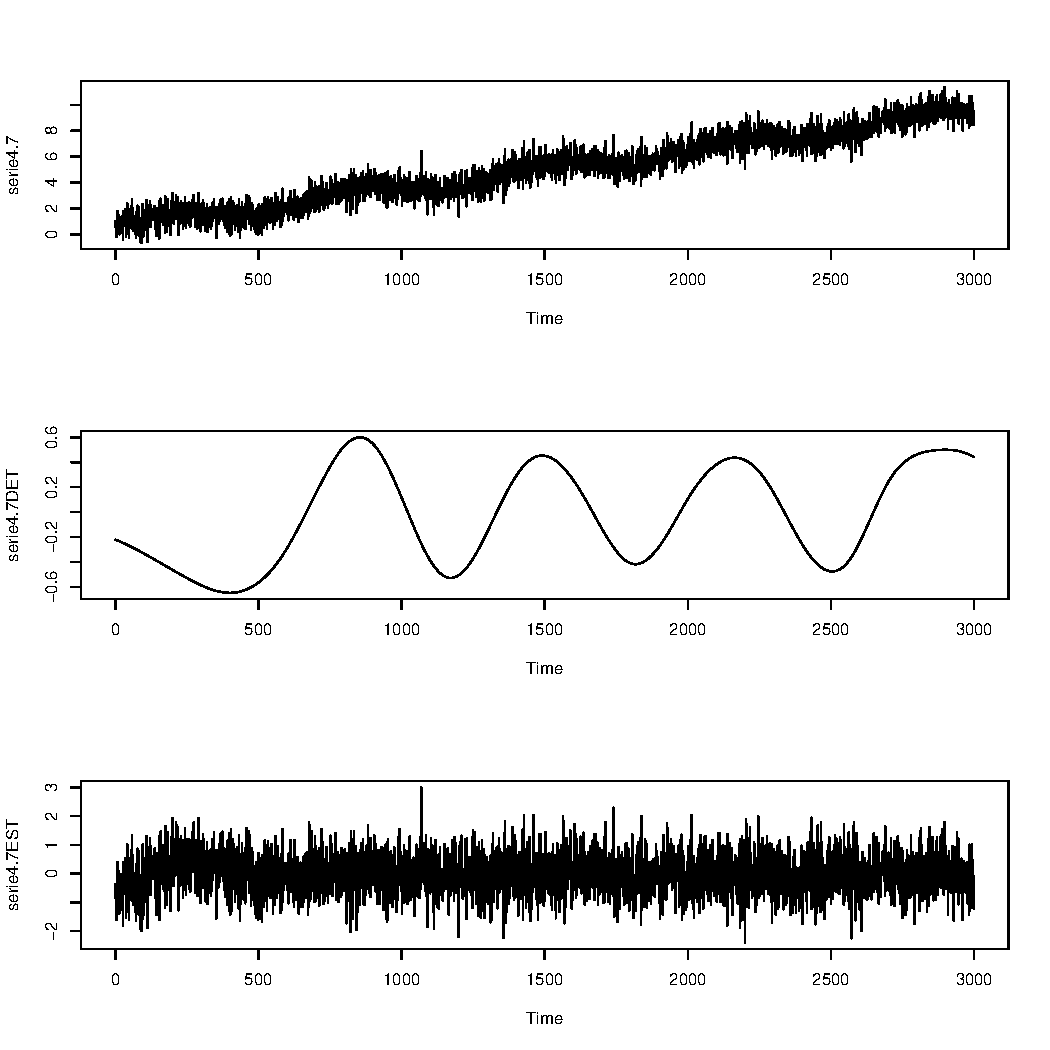
\includegraphics[scale=0.43]{serie4_7.pdf} \quad
  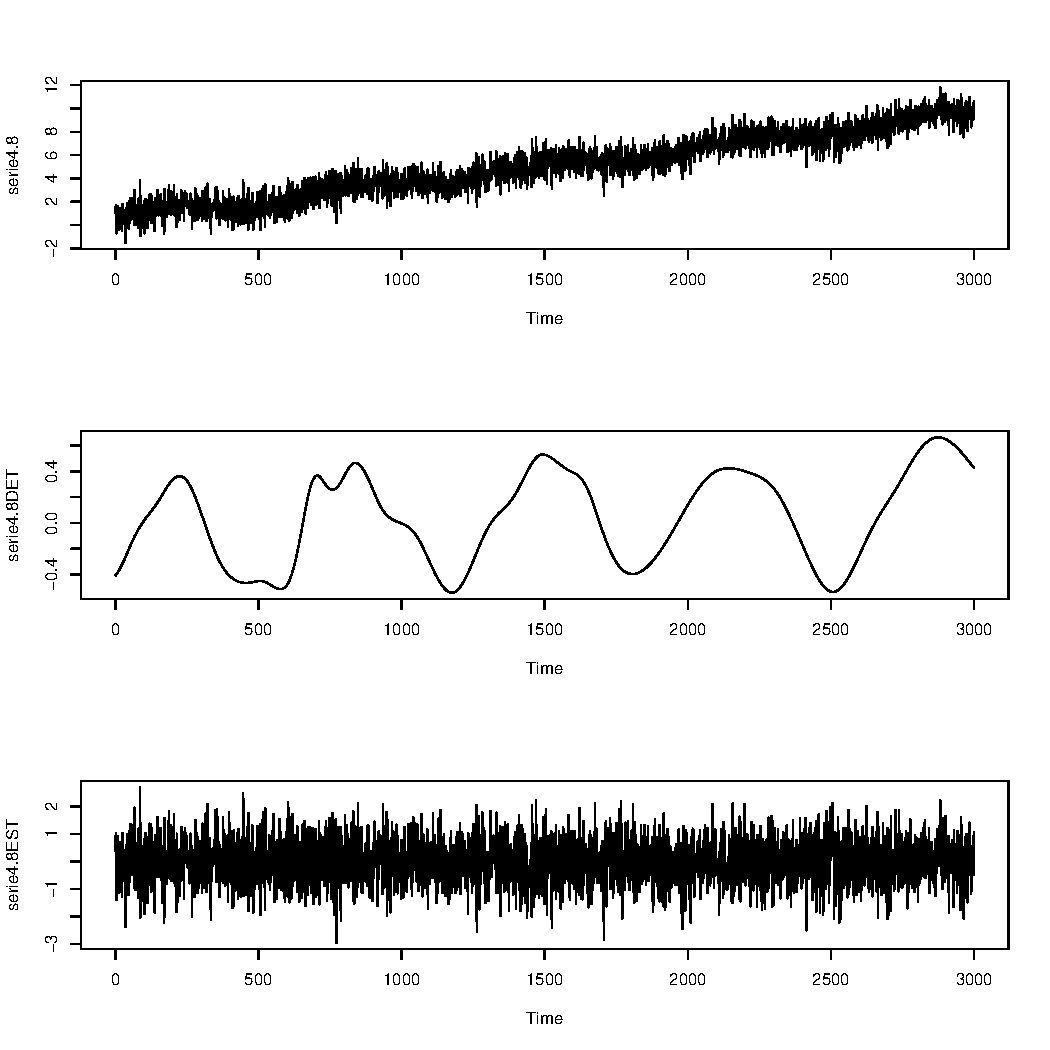
\includegraphics[scale=0.43]{serie4_8.pdf}
  \caption{Série 4.7 e Série 4.8}

\end{center}
\end{figure}

\graphicspath{{imagens/}}
\begin{figure}[H]
\begin{center}
  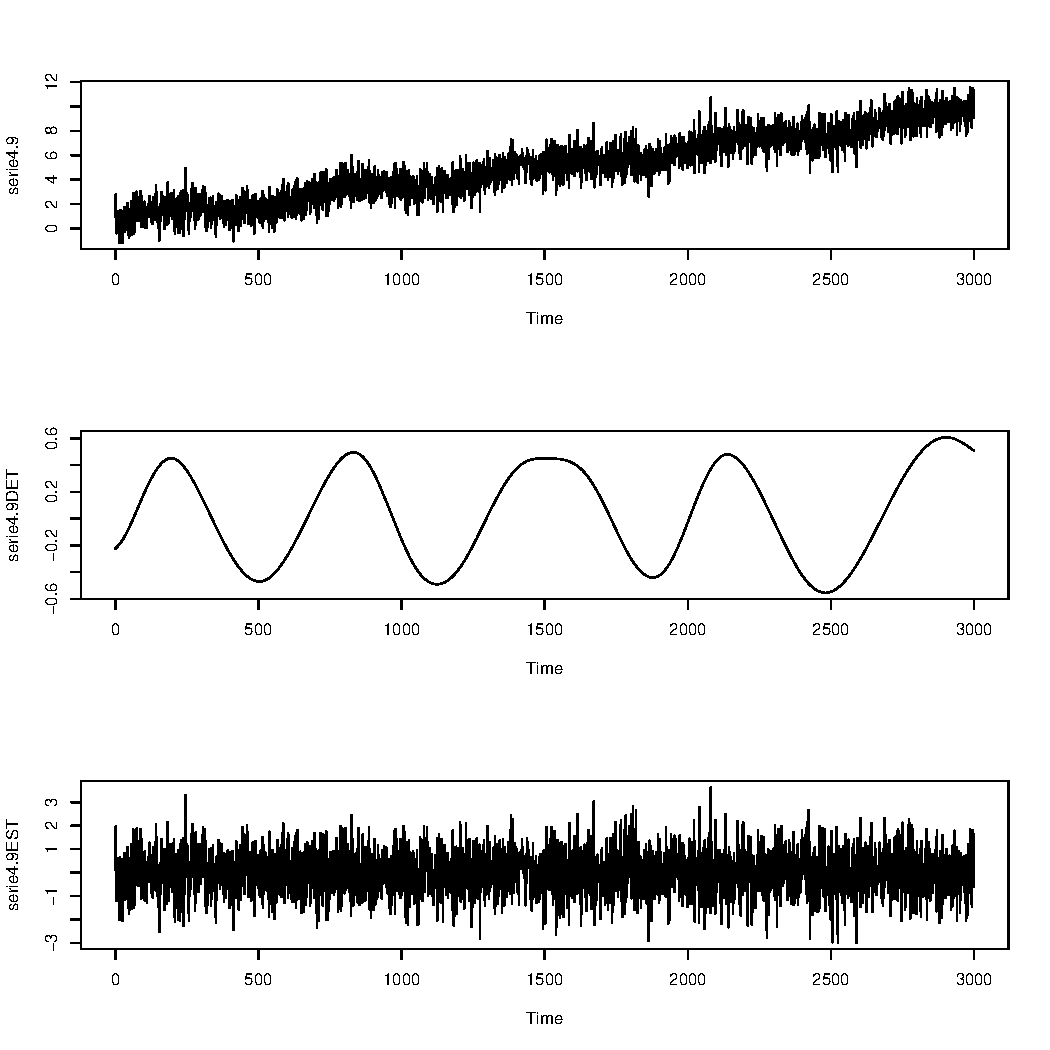
\includegraphics[scale=0.43]{serie4_9.pdf} \quad
  \includegraphics[scale=0.43]{serie4_10.pdf}
  \caption{Série 4.9 e Série 4.10}
\end{center}
\end{figure}
\section{Considerações Finais}
Foram apresentadas as séries temporais utilizadas neste trabalho experimental e suas respactivas decomposições.
% \include{apendice2}
% ...
% \include{apendiceM}

%% Fim do documento
\end{document}
%------------------------------------------------------------------------------------------%
